%%% Hlavní soubor. Zde se definují základní parametry a odkazuje se na ostatní části. %%%

%% Verze pro jednostranný tisk:
% Okraje: levý 40mm, pravý 25mm, horní a dolní 25mm
% (ale pozor, LaTeX si sám přidává 1in)
\documentclass[12pt,a4paper]{report}
\setlength\textwidth{145mm}
\setlength\textheight{247mm}
\setlength\oddsidemargin{15mm}
\setlength\evensidemargin{15mm}
\setlength\topmargin{0mm}
\setlength\headsep{0mm}
\setlength\headheight{0mm}
% \openright zařídí, aby následující text začínal na pravé straně knihy
\let\openright=\clearpage

%% Pokud tiskneme oboustranně:
% \documentclass[12pt,a4paper,twoside,openright]{report}
% \setlength\textwidth{145mm}
% \setlength\textheight{247mm}
% \setlength\oddsidemargin{14.2mm}
% \setlength\evensidemargin{0mm}
% \setlength\topmargin{0mm}
% \setlength\headsep{0mm}
% \setlength\headheight{0mm}
% \let\openright=\cleardoublepage

%% Vytváříme PDF/A-2u
\usepackage[a-2u]{pdfx}

%% Přepneme na českou sazbu a fonty Latin Modern
\usepackage[czech]{babel}
\usepackage{lmodern}
\usepackage[T1]{fontenc}
\usepackage{textcomp}

%% Použité kódování znaků: obvykle latin2, cp1250 nebo utf8:
\usepackage[utf8]{inputenc}

%%% Další užitečné balíčky (jsou součástí běžných distribucí LaTeXu)
\usepackage{amsmath}        % rozšíření pro sazbu matematiky
\usepackage{amsfonts}       % matematické fonty
\usepackage{amsthm}         % sazba vět, definic apod.
\usepackage{bbding}         % balíček s nejrůznějšími symboly
			    % (čtverečky, hvězdičky, tužtičky, nůžtičky, ...)
\usepackage{bm}             % tučné symboly (příkaz \bm)
\usepackage{graphicx}       % vkládání obrázků
\usepackage{fancyvrb}       % vylepšené prostředí pro strojové písmo
\usepackage{indentfirst}    % zavede odsazení 1. odstavce kapitoly
\usepackage{natbib}         % zajištuje možnost odkazovat na literaturu
			    % stylem AUTOR (ROK), resp. AUTOR [ČÍSLO]
\usepackage[nottoc]{tocbibind} % zajistí přidání seznamu literatury,
                            % obrázků a tabulek do obsahu
\usepackage{icomma}         % inteligetní čárka v matematickém módu
\usepackage{dcolumn}        % lepší zarovnání sloupců v tabulkách
\usepackage{booktabs}       % lepší vodorovné linky v tabulkách
\usepackage{paralist}       % lepší enumerate a itemize
\usepackage[usenames]{xcolor}  % barevná sazba

%%% Údaje o práci

% Název práce v jazyce práce (přesně podle zadání)
\def\NazevPrace{Tau Ceti f 2 – budovatelská počítačová hra se strategickými prvky}

% Název práce v angličtině
\def\NazevPraceEN{Tau Ceti f 2 – A Creative Computer Game with Strategic Elements}

% Jméno autora
\def\AutorPrace{Pavel Halbich}

% Rok odevzdání
\def\RokOdevzdani{2017}

% Název katedry nebo ústavu, kde byla práce oficiálně zadána
% (dle Organizační struktury MFF UK, případně plný název pracoviště mimo MFF)
\def\Katedra{Katedra distribuovaných a spolehlivých systémů}
\def\KatedraEN{Department of Distributed and Dependable Systems}

% Jedná se o katedru (department) nebo o ústav (institute)?
\def\TypPracoviste{Katedra}
\def\TypPracovisteEN{Department}

% Vedoucí práce: Jméno a příjmení s~tituly
\def\Vedouci{Mgr. Pavel Ježek, Ph.D.}

% Pracoviště vedoucího (opět dle Organizační struktury MFF)
\def\KatedraVedouciho{Katedra distribuovaných a spolehlivých systémů}
\def\KatedraVedoucihoEN{Department of Distributed and Dependable Systems}

% Studijní program a obor
\def\StudijniProgram{Informatika }
\def\StudijniObor{Programování a softwarové systémy}

% Nepovinné poděkování (vedoucímu práce, konzultantovi, tomu, kdo
% zapůjčil software, literaturu apod.)
\def\Podekovani{%
Děkuji mému vedoucímu Pavlu Ježkovi za pomoc s touto prací, mým rodičům za podporu a pevné nervy, mé přítelkyni Veronice taktéž za podporu a pomoc s 2D grafikou a Jiřímu Kurčíkovi za laskavé poskytnutí práv na použití jeho hudební tvorby v mé hře. 
}

% Abstrakt (doporučený rozsah cca 80-200 slov; nejedná se o zadání práce)
\def\Abstrakt{%
Abstrakt.
}
\def\AbstraktEN{%
Abstract.
}

% 3 až 5 klíčových slov (doporučeno), každé uzavřeno ve složených závorkách
\def\KlicovaSlova{%
{klíčová} {slova}
}
\def\KlicovaSlovaEN{%
{key} {words}
}

%% Balíček hyperref, kterým jdou vyrábět klikací odkazy v PDF,
%% ale hlavně ho používáme k uložení metadat do PDF (včetně obsahu).
%% Většinu nastavítek přednastaví balíček pdfx.
\hypersetup{unicode}
\hypersetup{breaklinks=true}

%% Definice různých užitečných maker (viz popis uvnitř souboru)
%%% Tento soubor obsahuje definice různých užitečných maker a prostředí %%%
%%% Další makra připisujte sem, ať nepřekáží v ostatních souborech.     %%%

%%% Drobné úpravy stylu

% Tato makra přesvědčují mírně ošklivým trikem LaTeX, aby hlavičky kapitol
% sázel příčetněji a nevynechával nad nimi spoustu místa. Směle ignorujte.
\makeatletter
\def\@makechapterhead#1{
  {\parindent \z@ \raggedright \normalfont
   \Huge\bfseries \thechapter. #1
   \par\nobreak
   \vskip 20\p@
}}
\def\@makeschapterhead#1{
  {\parindent \z@ \raggedright \normalfont
   \Huge\bfseries #1
   \par\nobreak
   \vskip 20\p@
}}
\makeatother

% Toto makro definuje kapitolu, která není očíslovaná, ale je uvedena v obsahu.
\def\chapwithtoc#1{
\chapter*{#1}
\addcontentsline{toc}{chapter}{#1}
}

% Trochu volnější nastavení dělení slov, než je default.
\lefthyphenmin=2
\righthyphenmin=2

% Zapne černé "slimáky" na koncích řádků, které přetekly, abychom si
% jich lépe všimli.
\overfullrule=1mm

%%% Makra pro definice, věty, tvrzení, příklady, ... (vyžaduje baliček amsthm)

\theoremstyle{plain}
\newtheorem{veta}{Věta}
\newtheorem{lemma}[veta]{Lemma}
\newtheorem{tvrz}[veta]{Tvrzení}

\theoremstyle{plain}
\newtheorem{definice}{Definice}

\theoremstyle{remark}
\newtheorem*{dusl}{Důsledek}
\newtheorem*{pozn}{Poznámka}
\newtheorem*{prikl}{Příklad}

%%% Prostředí pro důkazy

\newenvironment{dukaz}{
  \par\medskip\noindent
  \textit{Důkaz}.
}{
\newline
\rightline{$\square$}  % nebo \SquareCastShadowBottomRight z balíčku bbding
}

%%% Prostředí pro sazbu kódu, případně vstupu/výstupu počítačových
%%% programů. (Vyžaduje balíček fancyvrb -- fancy verbatim.)

\DefineVerbatimEnvironment{code}{Verbatim}{fontsize=\small, frame=single}

%%% Prostor reálných, resp. přirozených čísel
\newcommand{\R}{\mathbb{R}}
\newcommand{\N}{\mathbb{N}}

%%% Užitečné operátory pro statistiku a pravděpodobnost
\DeclareMathOperator{\pr}{\textsf{P}}
\DeclareMathOperator{\E}{\textsf{E}\,}
\DeclareMathOperator{\var}{\textrm{var}}
\DeclareMathOperator{\sd}{\textrm{sd}}

%%% Příkaz pro transpozici vektoru/matice
\newcommand{\T}[1]{#1^\top}

%%% Vychytávky pro matematiku
\newcommand{\goto}{\rightarrow}
\newcommand{\gotop}{\stackrel{P}{\longrightarrow}}
\newcommand{\maon}[1]{o(n^{#1})}
\newcommand{\abs}[1]{\left|{#1}\right|}
\newcommand{\dint}{\int_0^\tau\!\!\int_0^\tau}
\newcommand{\isqr}[1]{\frac{1}{\sqrt{#1}}}

%%% Vychytávky pro tabulky
\newcommand{\pulrad}[1]{\raisebox{1.5ex}[0pt]{#1}}
\newcommand{\mc}[1]{\multicolumn{1}{c}{#1}}


%% Titulní strana a různé povinné informační strany
\begin{document}
%%% Titulní strana práce a další povinné informační strany

%%% Titulní strana práce

\pagestyle{empty}
\hypersetup{pageanchor=false}

\begin{center}

\centerline{\mbox{
\includegraphics[width=166mm]{../img/logo-cs.pdf}}}

\vspace{-8mm}
\vfill

{\bf\Large BAKALÁŘSKÁ PRÁCE}

\vfill

{\LARGE\AutorPrace}

\vspace{15mm}

{\LARGE\bfseries\NazevPrace}

\vfill

\Katedra

\vfill

\begin{tabular}{rl}

Vedoucí bakalářské práce: & \Vedouci \\
\noalign{\vspace{2mm}}
Studijní program: & \StudijniProgram \\
\noalign{\vspace{2mm}}
Studijní obor: & \StudijniObor \\
\end{tabular}

\vfill

% Zde doplňte rok
Praha \RokOdevzdani

\end{center}

\newpage

%%% Následuje vevázaný list -- kopie podepsaného "Zadání bakalářské práce".
%%% Toto zadání NENÍ součástí elektronické verze práce, nescanovat.

%%% Strana s čestným prohlášením k bakalářské práci

\openright
\hypersetup{pageanchor=true}
\pagestyle{plain}
\pagenumbering{roman}
\vglue 0pt plus 1fill

\noindent
Prohlašuji, že jsem tuto bakalářskou práci vypracoval(a) samostatně a výhradně
s~použitím citovaných pramenů, literatury a dalších odborných zdrojů.

\medskip\noindent
Beru na~vědomí, že se na moji práci vztahují práva a povinnosti vyplývající
ze zákona č. 121/2000 Sb., autorského zákona v~platném znění, zejména skutečnost,
že Univerzita Karlova má právo na~uzavření licenční smlouvy o~užití této
práce jako školního díla podle §60 odst. 1 autorského zákona.

\vspace{10mm}

\hbox{\hbox to 0.5\hsize{%
V ........ dne ............
\hss}\hbox to 0.5\hsize{%
Podpis autora
\hss}}

\vspace{20mm}
\newpage

%%% Poděkování

\openright

\noindent
\Podekovani

\newpage

%%% Povinná informační strana bakalářské práce

\openright

\vbox to 0.5\vsize{
\setlength\parindent{0mm}
\setlength\parskip{5mm}

Název práce:
\NazevPrace

Autor:
\AutorPrace

\TypPracoviste:
\Katedra

Vedoucí bakalářské práce:
\Vedouci, \KatedraVedouciho

Abstrakt:
\Abstrakt

Klíčová slova:
\KlicovaSlova

\vss}\break\vbox to 0.49\vsize{
\setlength\parindent{0mm}
\setlength\parskip{5mm}

Title:
\NazevPraceEN

Author:
\AutorPrace

\TypPracovisteEN:
\KatedraEN

Supervisor:
\Vedouci, \KatedraVedoucihoEN

Abstract:
\AbstraktEN

Keywords:
\KlicovaSlovaEN

\vss}

\newpage

\openright
\pagestyle{plain}
\pagenumbering{arabic}
\setcounter{page}{1}


%%% Strana s automaticky generovaným obsahem bakalářské práce

\tableofcontents

%%% Jednotlivé kapitoly práce jsou pro přehlednost uloženy v samostatných souborech
%!TEX root = ../../prace.tex

\chapter{Úvod}

V době vzniku této práce jsou velice populární hry s~otevřeným světem. Lákají hráče na obsáhlost světa a~možnost nelineárního řešení problémů a~herních úkolů. Her s~otevřeným světem najdeme nepřeberné množství v~různých herních žánrech. My se zaměříme na podmnožinu her, které kromě otevřeného světa nabízí také možnosti budování struktur a~vyžadují od hráče netriviální styl hraní, který mu umožňuje ve hře přežít. V herním průmyslu se tyto hry často označují jako \textit{sanboxové}, \textit{s budováním}, \textit{s průzkumem prostředí}, \textit{o přežití}. Autor této práce má tento typ her v~oblibě a~rád by touto prací představil svoji vizi dalšího možného rozvoje her tohoto žánru. Cílem práce by měla být implementace nového herního principu stavění, které současné herní tituly nenabízí.

\section{Charakteristika her}
V práci se budeme zabývat několika různými hrami, které však mají několik společných vlastností. Jedním ze základních konceptů je využívání herních bloků. Dalším význačným prvkem je způsob integrace herních bloků do herního prostření. Některé hry jsou celé tvořeny bloky, jiné se snaží dosáhnout vyššího stupně realismu ve hře a~bloky využívají pouze pro konstrukci různých herních objektů. Důležitým tématem této práce tedy bude rozbor systému bloků a~práce s~nimi a~popis hráčských problémů způsobených danými koncepty. V další části práce pak navrhneme a~implementujeme vlastní řešení.




\subsection{Hry kompletně blokové}
Začněme hrami, které využívají bloků jako základního elementu celé hry. Bloky zde tvoří doslova celý svět. Mezi nejpopulárnější a~širokou veřejností nejznámější bychom měli zařadit hru \MC{}. Na obrázku z této hry \ref{fig:intro_mc} si můžeme všimnout několika zásadních faktů. Vidíme zde kostičkované listí stromů (1) či hrad na skále (2), který byl postaven z~kostiček. Taktéž slunce, měsíc a~mraky (3) jsou stylizovány do kostiček. Výrazně je kostičkovaný styl vidět na nehratelných postavách (\textit{non-playable character} -- \NPC{}) -- na obrázku ovce (4), krávy a~prasata. Stejným způsobem je pak zpracován i~hráčův charakter (5), tedy postava, kterou hráč přímo ovládá.

TODO zmínit crafting, stavěnbí

\begin{figure}[!ht]\centering
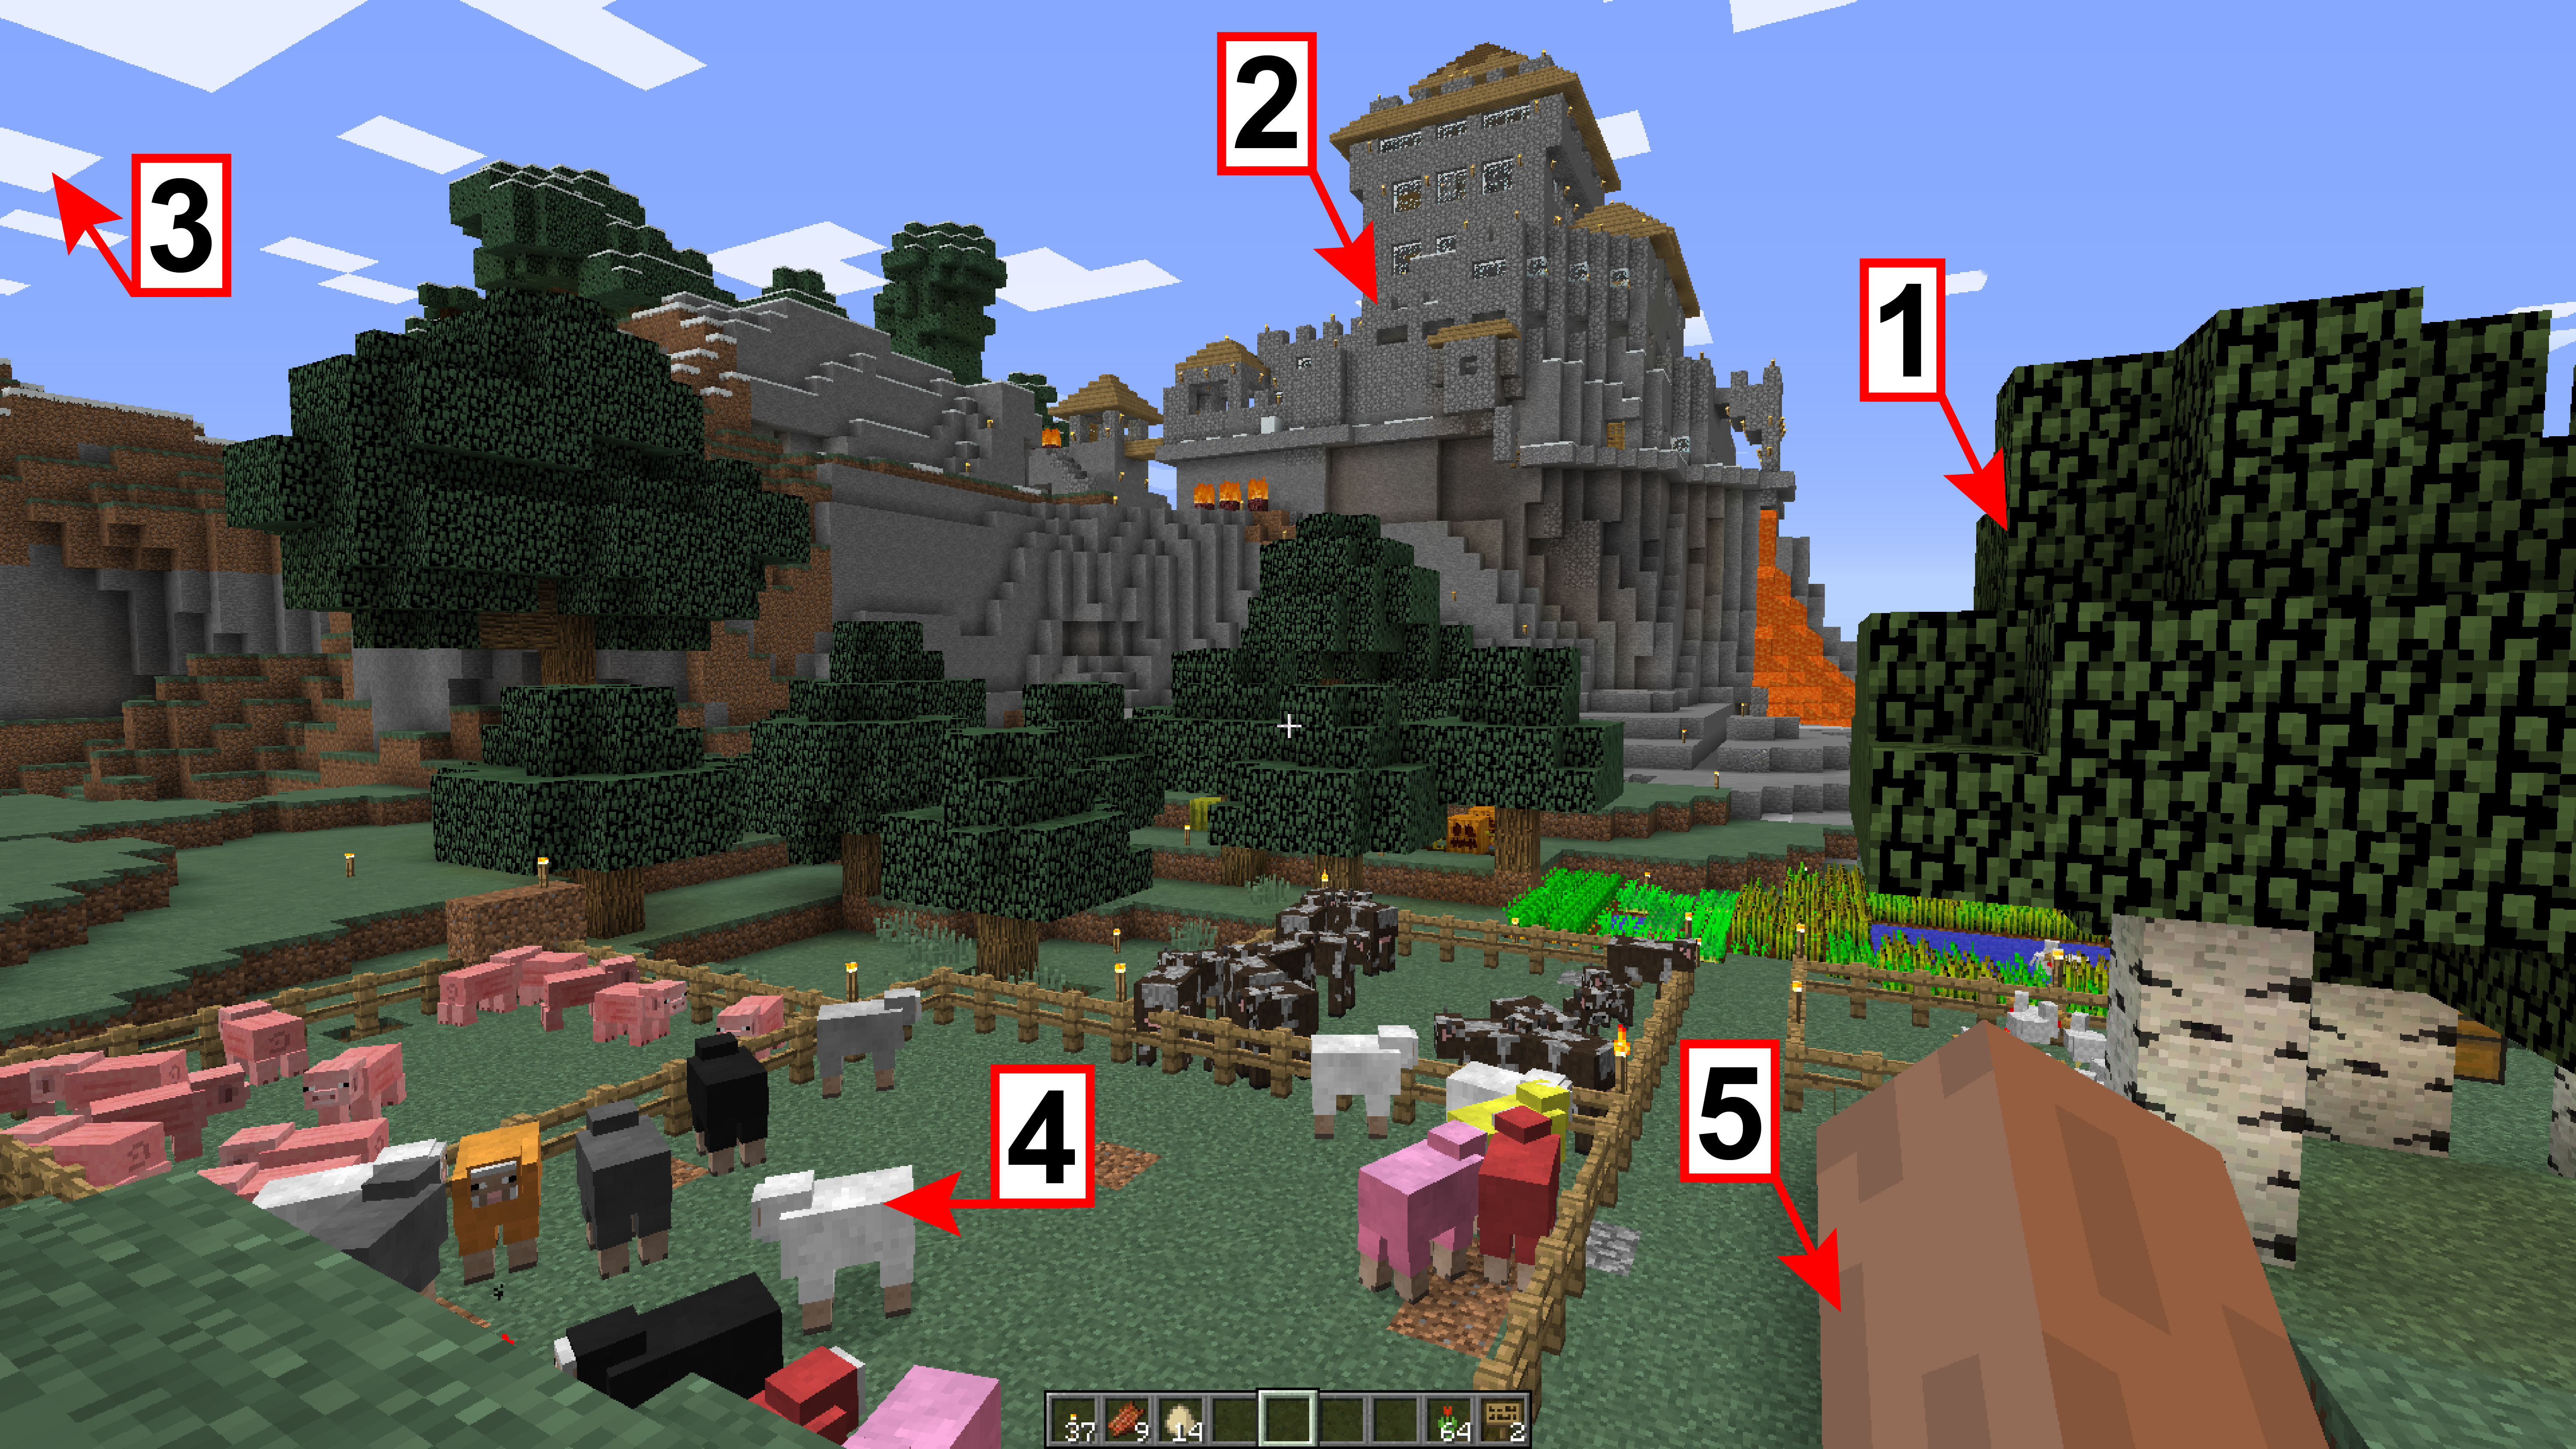
\includegraphics[ width=140mm]{../img/intro/mc}

\caption{Hra Minecraft - hrad na skále}
\label{fig:intro_mc}

\end{figure}

\FloatBarrier

Mezi dalšími hrami bychom mohli zmínit například \TE{}. Ta je o~něco mladší než \MC{}, ale je častým zdrojem diskusí, zda je lepší new \MC{}, nebo ne. Pravdou je, že obě hry mají svůj svět kompletně složený z~kostek (\TE{} je však 2D hra), ale každá si klade trochu jiné cíle. \TE{} je více orientovaná na příběh, obsahuje více \NPC{} i~bossů. Boss je v~herní terminologii významný nepřítel, obvykle je silnější než ostatní protivníci a~velmi často bývá v~závěrečných částech hry. Duel s~bossem pak obvykle od hráče vyžaduje zjištění jeho silných a~slabých stránek a~schémat jeho útoků \citep{intro_boss}. \MC{} je pak orientován spíše na stavění. (Porovnání Minecraft vs Terraria (facts) \citep{mc_te_comparsion} na Minecraftovém fóru.)


\subsection{Hry s~prvky realismu}

Mezi hry s~prvky realismu bychom mohli zařadit třeba hry \SE{} či \ME{}, využívají kombinaci herních bloků s~\textit{voxelovou} reprezentací světa. Obě hry jsou implementovány v~proprietárním enginu společnosti Keen Software House nazvaném \textit{VRAGE}\texttrademark{}. Voxelový terén je pak v~enginu za běhu hry procedurálně generován do polygonální reprezentace, kterou pak grafická karta standardním způsobem vykreslí na obrazovce (oficiální popis vlastností enginu \citep{vrage}). Během tohoto procedurálního vytváření je na třídimenzionální strukturu voxelů (které si můžeme představit jako bloky stejné velikosti) aplikován nějaký šum a~tím je možné ve hře vygenerovat prakticky neomezené množství různých objektů vycházejících z~jedné voxelové struktury. \uv{\textit{The “procedural asteroids” feature adds a~practically infinite number of asteroids to the game world}} \citep{rosa_blog}. Tímto způsobem pak hry dosáhují vyššího stupně realismu -- nespoléhají se pouze na předpřipravené 3D modely. 

Podívejme se na obrázek \ref{fig:intro_se} ze hry \SE{}. Na něm můžeme vidět převážně kamenný asteroid, a na něm je postavená vesmírná základna (obarvená zelenou barvou). K základně je přistavena větší vesmírná loď (modrobílá, v~levém horním rohu), hráč pak k~základně letí v~další, malé lodi (modrobílá uprostřed). Bližší pohled na planetku ukazuje, že její povrch není pravidelný. To je způsobeno právě algoritmickou aproximací voxelové reprezentace planetky. 

\begin{figure}[!ht]\centering
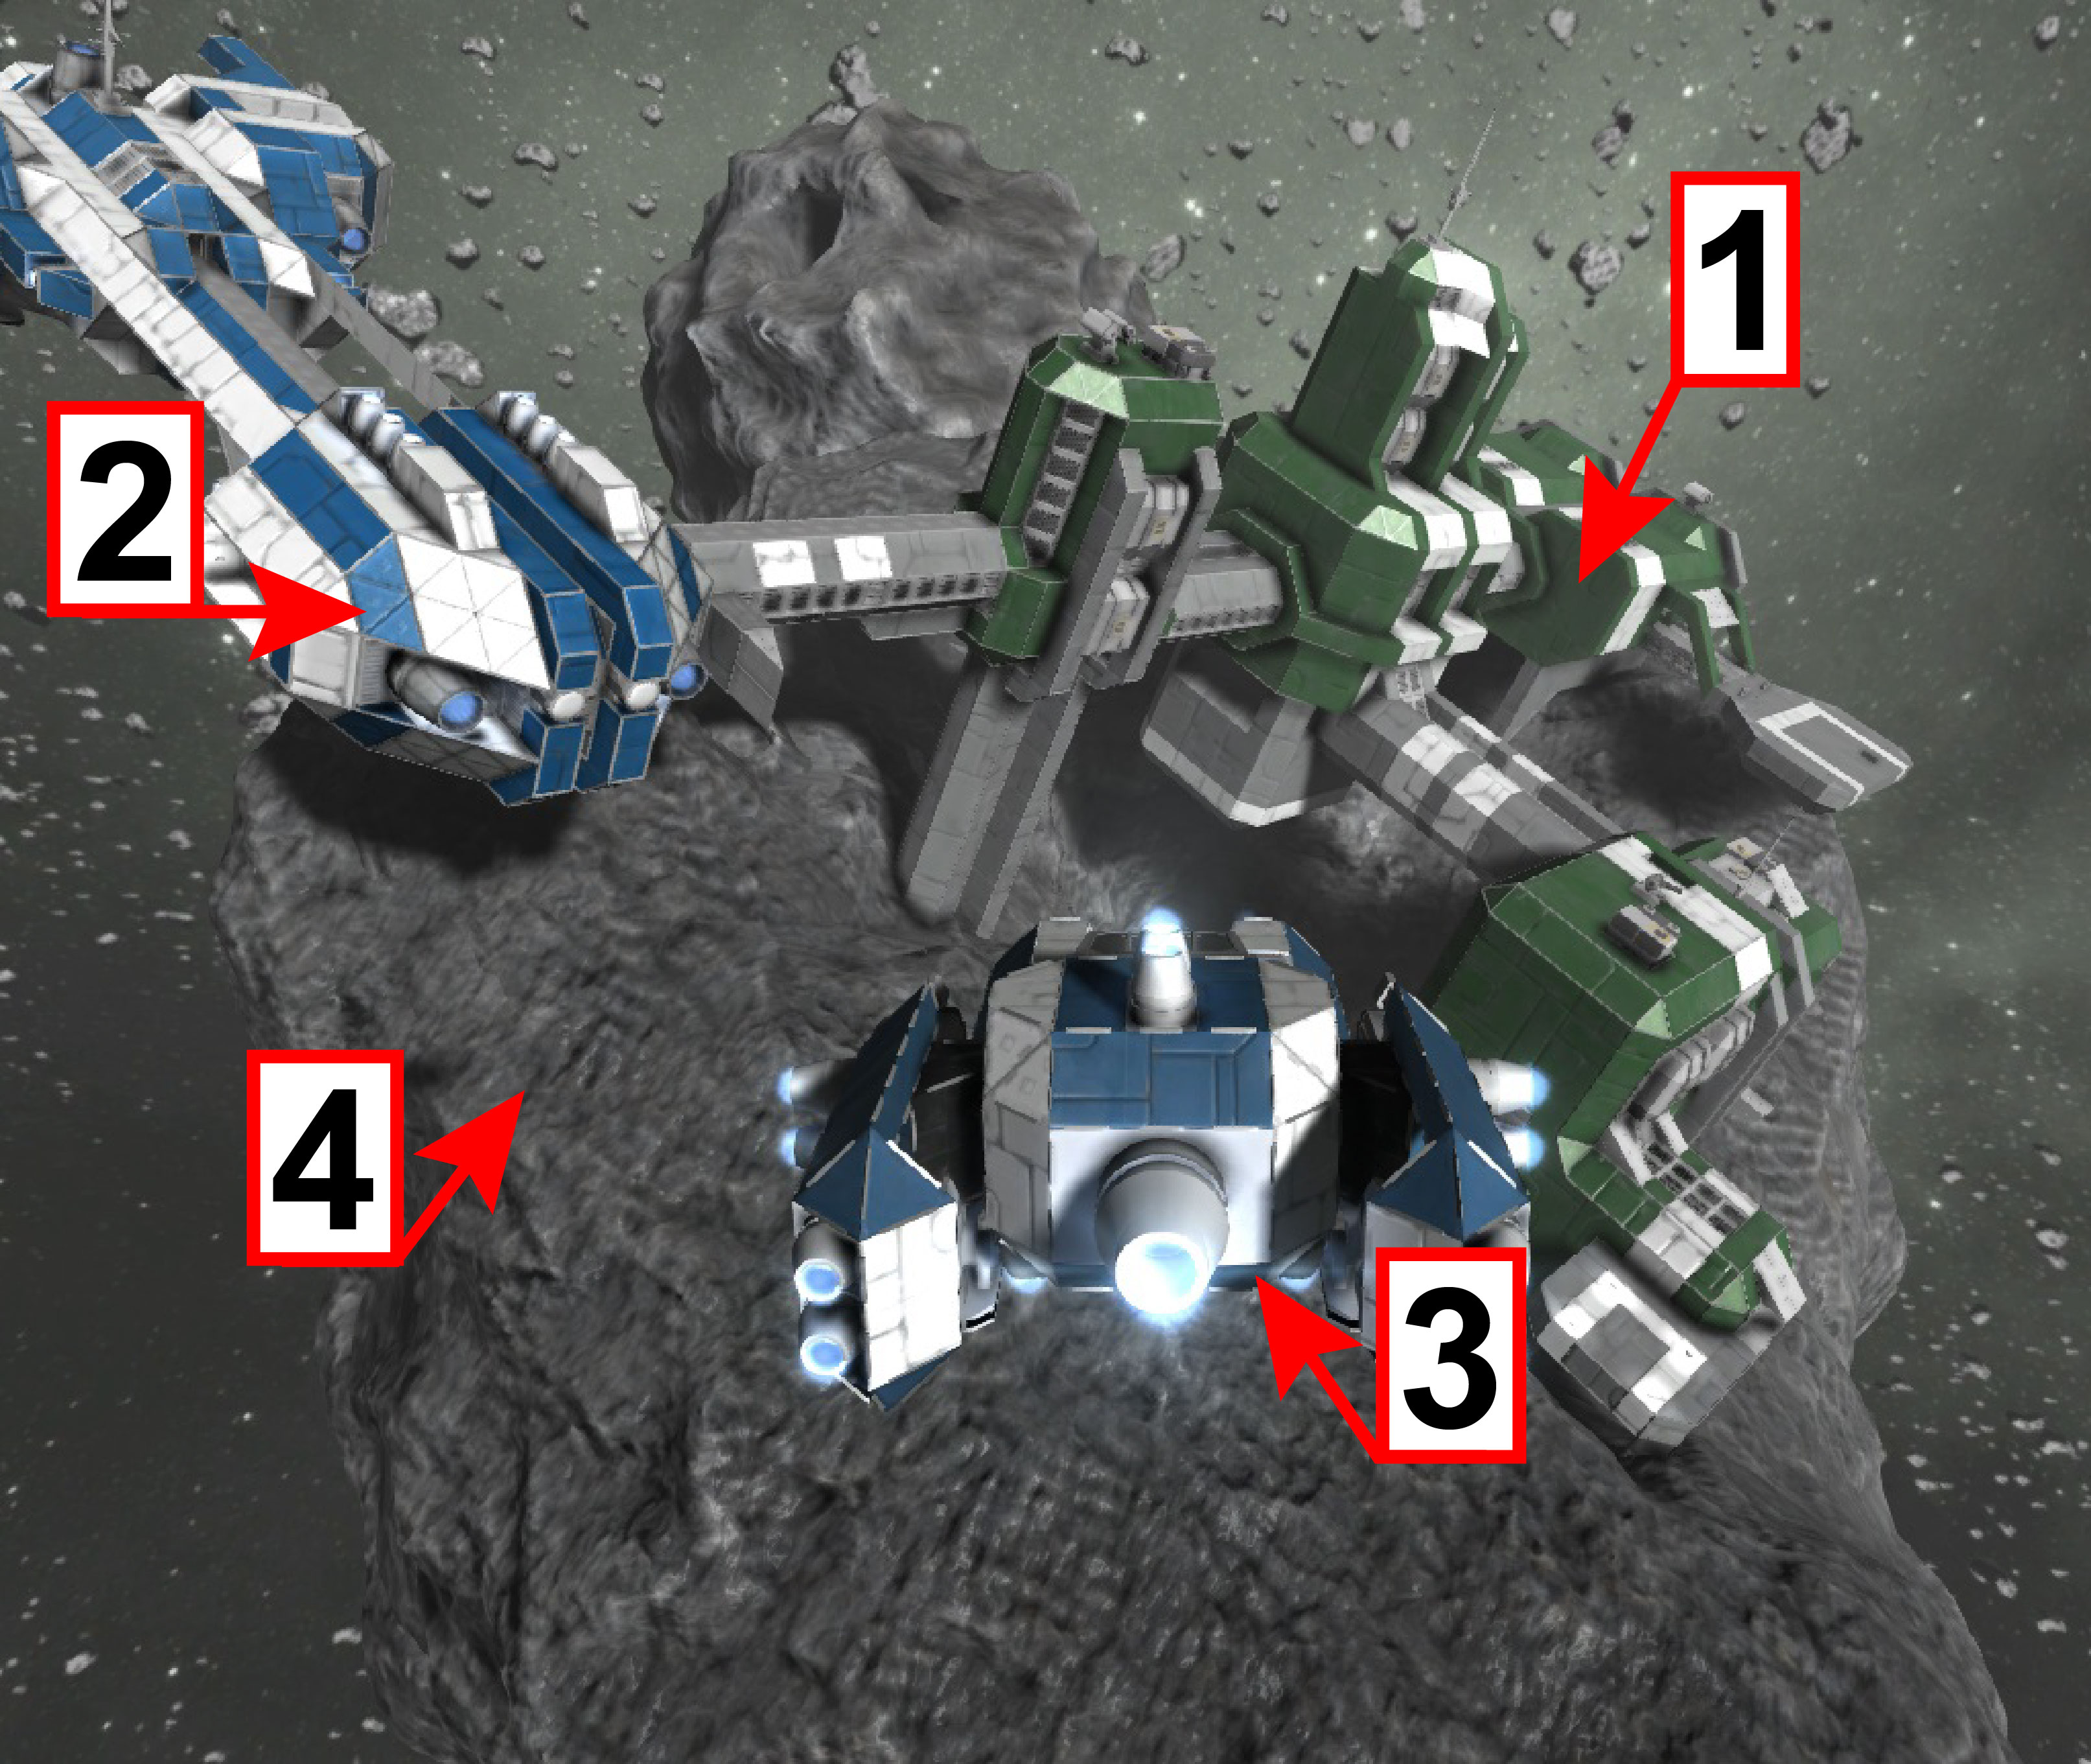
\includegraphics[ width=140mm]{../img/intro/se}

\caption{Hra Space Engineers -- základna. Zdroj: Gamespot.com \citep{se_intro_img} }
\label{fig:intro_se}

\end{figure}

\FloatBarrier

Samotná základna i~vesmírná plavidla (detailní pohled na jiné plavidlo je na obrázku \ref{fig:intro_se_ship}) jsou tvořeny bloky. Vizuální reprezentace bloku může být i~jiného tvaru než jen krychle -- to je možné vidět na obrázku \ref{fig:intro_se_blocks}). Barevně jsou zde zvýrazněny hranice bloků. Jak základny, tak vesmírné lodě (které jsou navíc oproti základnám pohyblivé) využívají tento systém. 

\SE{} umožňuje stavět pohyblivé stroje, které si hráč postaví z~herních bloků a~ty se pak chovají jako jedna entita. Stále je na ně však aplikována fyzika, takže je možné plavidlo poškodit, nebo dokonce zničit. Tento stupeň realismu od naší hry vyžadovat nebudeme. Budeme však chtít mít ve hře bloky, jejichž model není tvaru krychle. Stejně jako v \SE{} budeme chtít, aby bylo možné bloky rotovat v libovolném směru (u bloků, u kterých to bude dávat smysl).


TODO zmínit crafting, stavěnbí, conveyor systém

\begin{figure}[!ht]\centering
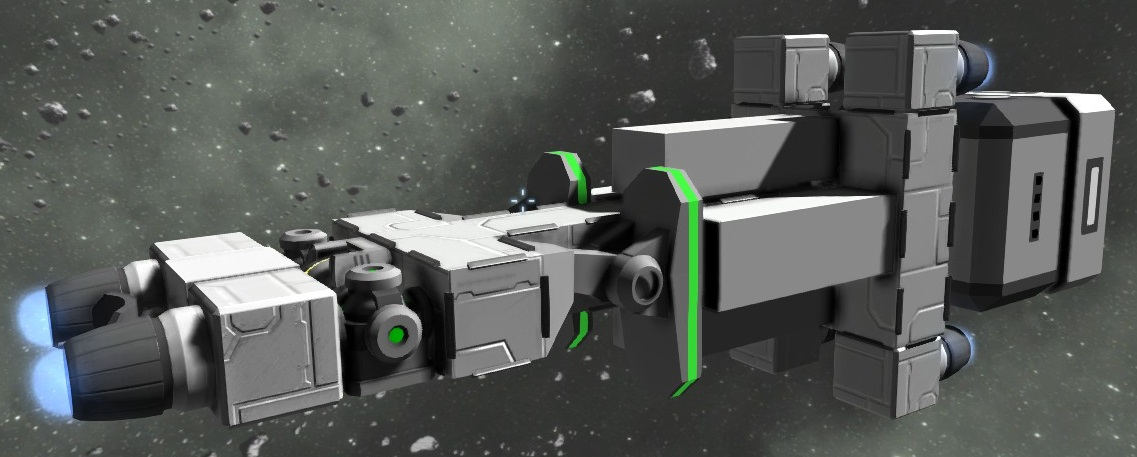
\includegraphics[ width=140mm]{../img/intro/se_ship}

\caption{Hra Space Engineers -- dron. Zdroj: space-engineer.net \citep{se_drone_source}}
\label{fig:intro_se_ship}

\end{figure}

\begin{figure}[!ht]\centering
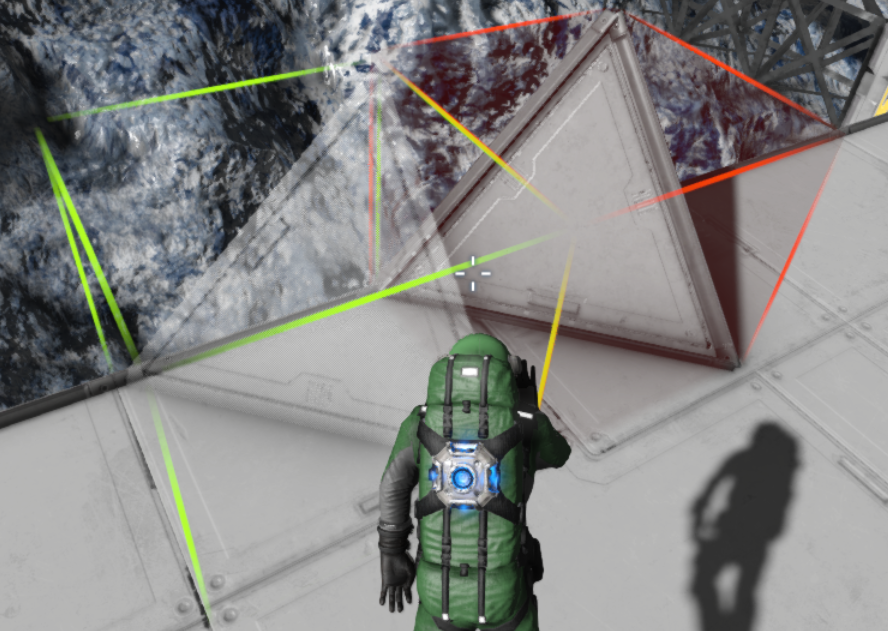
\includegraphics[ width=140mm]{../img/intro/se_blocks}

\caption{Hra Space Engineers - bloky }
\label{fig:intro_se_blocks}

\end{figure}

\FloatBarrier


\subsection{Hry s~maximálním důrazem na simulaci reality}

Do této sekce bychom měli zařadit například vesmírný simulátor \TM{}. // TODO popis, obrázek

Zmínit stavění

\begin{figure}[!ht]\centering
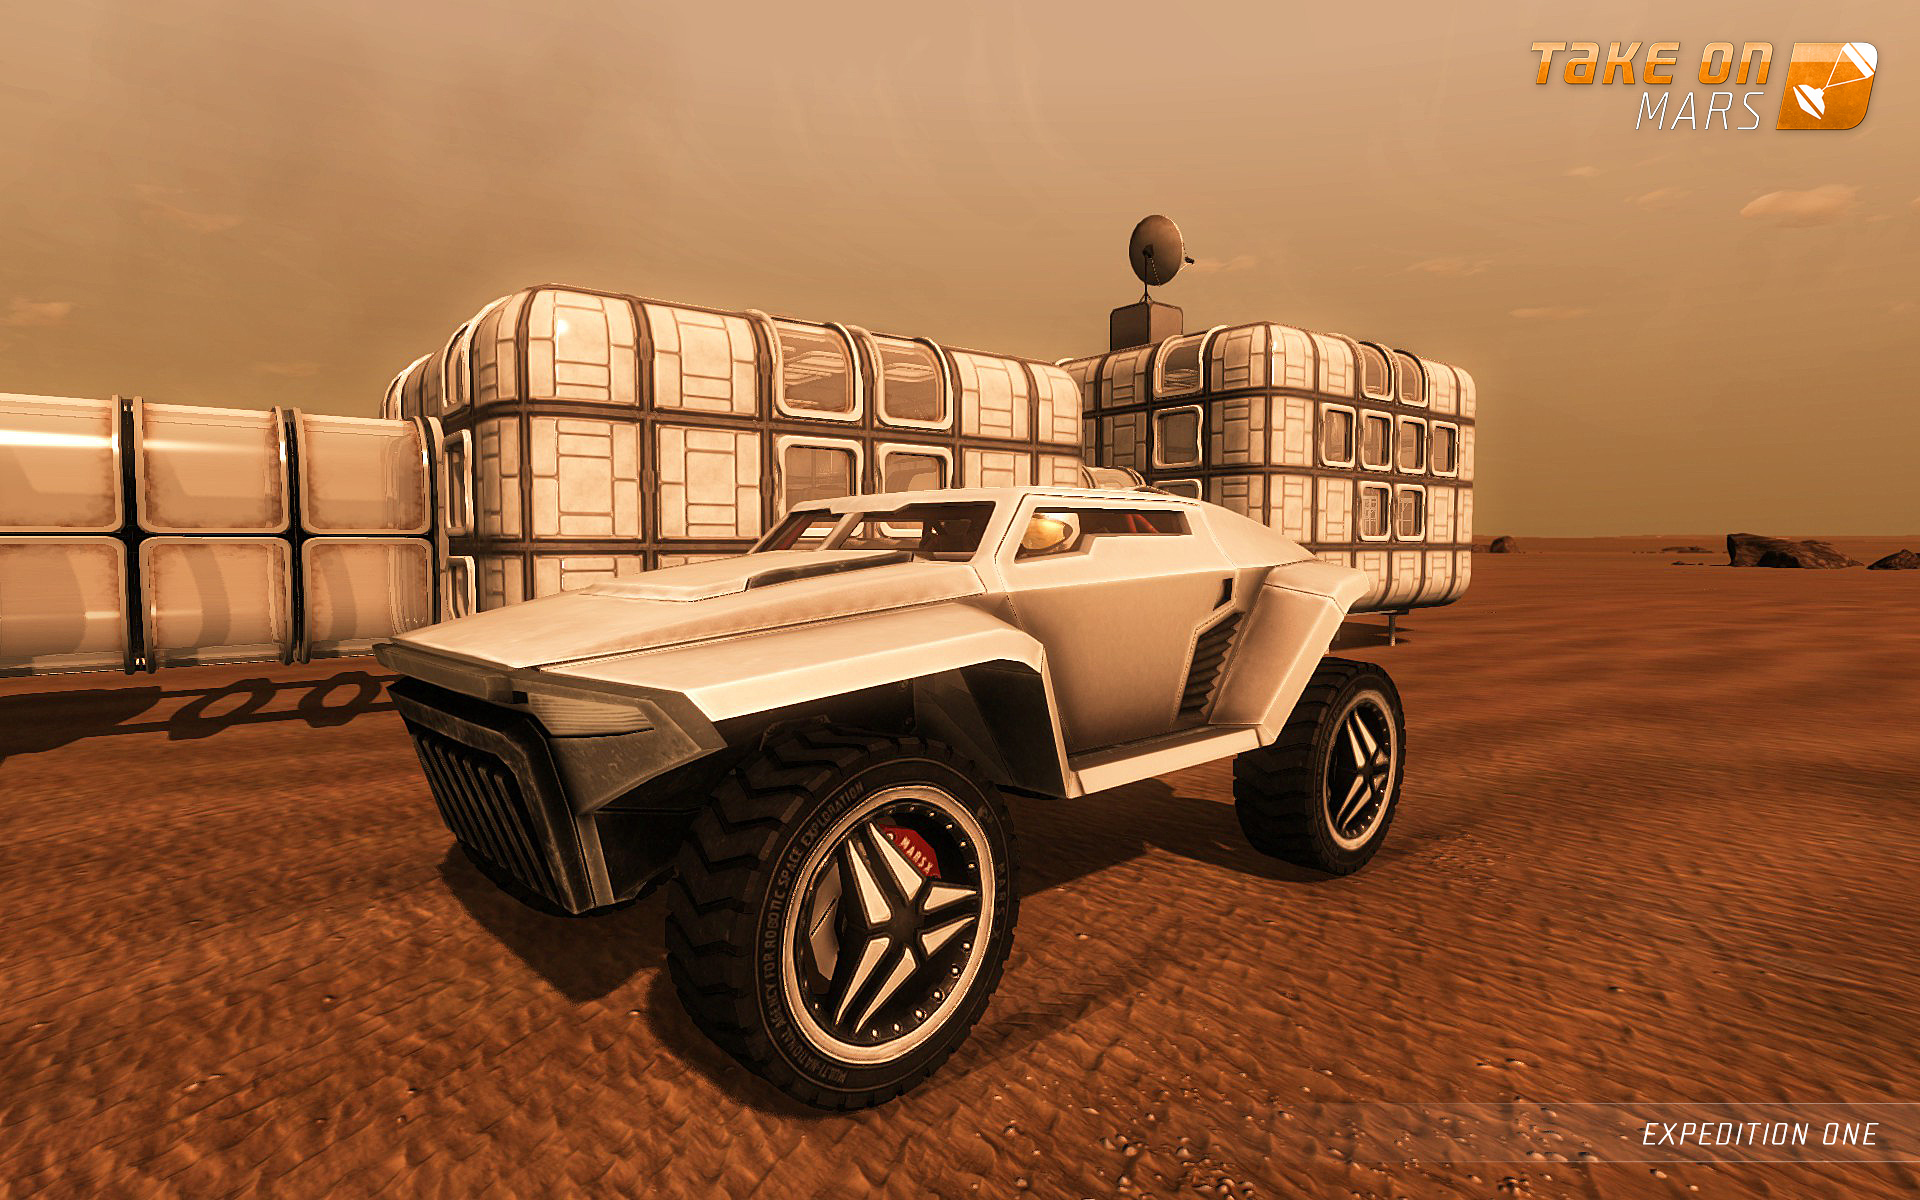
\includegraphics[ width=140mm]{../img/intro/tom}

\caption{Hry Take On Mars -- vozítko před budovou. Zdroj: Hry.cz \citep{intro_tom_source}}
\label{fig:intro_tom}

\end{figure}

\FloatBarrier

bloky na stavění, ale třeba vozidla kompletní

\subsection{Ostatní - zařadit TODO }

Můžeme však nalézt i~další příklady her (// TODO , , , , ).

\NI{}
Novus incpetio je MMORPG, stavění https://www.youtube.com/watch?v=d2ySkvn6wyw probíhá tím stylem, že se hráč přepne do build módu, vše si naplánuje (va výdledek vidí rovnou tak, jak bude vypadat). Po ukončení toho módu pak hráč vidí obrysy naplánovaných bloků. (Ty se přichytávají do mřížky a k sobě) Pak je může začít konstruovat, přičemž v nabídce během konstrukce má možnost si chybějící součásti craftnout.


\PN{}

https://www.youtube.com/watch?v=Wpurqr3YaGQ funguje podobně jako Space engineers - získávání surovin, kraftění na komponenty a použřívání komponent na konstrukci objetků. POstavený objekt ukazuje základní konstrukci.


\ARK{}
Ark počáteční free point, pak se bloky přidávají k sobě https://www.youtube.com/watch?v=TOmjjo5QoP8 


\NMS{}
Stejně jako \TM{} používá snappointy

\section{Čemu se budeme věnovat}

Rádi bychom zachovali koncept použití herních bloků, který shledáváme jednoduchý na pochopení i~použití. Zaměříme se na rozšíření možnosti práce s~bloky tak, abychom uživateli nabídli, pokud možno, ještě lepší herní zážitek ze stavění vlastních výtvorů. V této práci se nebudeme nijak důkladně věnovat vizuální reprezentaci prostředí, protože ta pro nás v~tuto chvíli není podstatná. 

Změna v~přístupu k~herním blokům bude vyžadovat i~úpravy herního mechanismu s~tím souvisejícího -- hráčova inventáře. Všechny výše zmíněné hry nějakým způsobem nabízí hráči výběr bloků, které může do herního světa umístit. Naše změna by bohužel znamenala, že by se takový inventář postavitelných bloků velmi rychle stal nepřehledným a~proto musíme systém nabídky postavitelných bloků upravit pro naše potřeby.

\section{Herní bloky}



Obvykle je ve hře definován jeden základní rozměr bloku, který je neměnný. (\SE{} definuje více velikostí -- ty však nelze vzájemně kombinovat). To však může být problémem, pokud se hráč rozhodne postavit v~herním světě nějakou větší a~komplexnější strukturu podle reálné či fiktivní předlohy. Pro příklad uveďme některé výtvory ze hry \MC{} -- město Královo přístaviště z~knih Píseň ledu a~ohně od Geoge R. R. Martina, nebo hlavní město Gondoru Minas Tirith z~knih Pána prstenů od J. R. R. Tolkiena.

Autoři těchto výtvorů museli volit takové měřítko, aby byly výtvory dostatečně detailní, ale zároveň aby bylo možné výtvor postavit v~nějakém rozumném čase. Obecně můžeme říct, že čím větších detailů chtějí autoři ve hře \MC{} dosáhnout, tím větší musí celý výtvor být. To pak ale znamená, že celá stavba trvá déle, nebo je zapotřebí více spolupracujících hráčů. Hra \SE{} díky svému přístupu a~více bloků, které nejsou tvaru krychle, nabízí lepší možnosti staveb rozsáhlých objektů (představme si třeba Hvězdu smrti z~Hvězných válek), ale stále je potřeba volit nějakou rozumnou výslednou velikost.


\subsection{Náš návrh úpravy}
Chtěli bychom se v~této práci zabývat myšlenkou proměnlivé velikosti stavitelných bloků. Tím by hráči mohli rychleji stavět rozsáhlejší struktury a~přitom se věnovat i~drobným či estetickým detailům. Tento návrh však s~sebou nese několik problémů, které se v~této práci budeme snažit vyřešit.


\section{Inventář}
Dalším společným prvkem tohoto druhu her je inventář bloků, které může hráč umístit do herního světa. Hráč přes celé herní okno vidí \HUD{} (Head-Up Display \citep{hud_terminology}), ve kterém má zobrazenou kromě jiného nabídku bloků, které má na rychlé volbě, může je snadno zvolit a~daný blok umístit do herního světa. Navíc hry mohou definovat i~inventární skupiny bloků (\SE{}, \ME{}), mezi kterými hráč může přepínat a~tím rychle kompletně změnit sadu rychlé nabídky. Vidíme však limitaci v~tom, že hráč musí ručně spravovat tyto seznamy a~jednotlivé bloky (či nástroje) umisťovat do příslušných pozic.


\subsection{Náš návrh úpravy}
Rádi bychom navrhli jiný způsob správy těchto inventárních skupin, aby hráč jednou definoval, jaké prvky chce mít v~příslušných skupinách. Při vytvoření nového bloku či vytvoření jiné velikosti bloku by pak nemusel ručně přiřazovat nový blok do skupiny, ale tento blok by měl být automaticky zařazen a~nabídnut hráči.  




\section{Cíle práce}
Tato práce by měla naplnit následující cíle:
\begin{itemize}
	\item Navrhnout a~implementovat způsob řešení proměnlivé velikosti bloků
	\item Navrhnout a~implementovat automatizovanou správu inventáře
	\item Kvůli očekávaným nárokům na pochopení nových konceptů do hry implementovat výukový tutoriál (TODO má to být tady?)
	\item Získat a~zhodnotit zpětnou vazbu na výslednou hru
\end{itemize}


%!TEX root = ../prace.tex

\chapter{Analýza zadání}

\section{Stávající implementace mechanismů}
- v dalším textu budeme vycházet z her: \\

Minecraft \\
Space Engineers / Medieval Engineers \\

\begin{itemize}
	\item popsat, jak je to v jednotlivých zmíněných hrách (musel jsem je nutně hrát všechny?)
	\item popsat velikosti bloků, nějaké zákonitosti, fyziku
	\item popsat strategické mechaniky
\end{itemize}

\section{Rozbor zadání}

Zde bychom měli popsat, co by se nám ve hře líbilo a stanovit reálnost implementace
\\

Nejspíše se text bude prolínat s kapitolou - dalším vývojem?\\
Měl bych si tu vysnit celou hru, nebo to spíše seškrtat?


\begin{itemize}
	\item tedy že bychom chtěli panďuláka, jaké pohledy
	\item a že bychom s ním chtěli chodit a stavět a bourat
	\item ale že nám taky může umřít - počasí, kyslík
	\item popsat svět, bloky, co by asi měly umět

\end{itemize}


\section{Cíle práce}
%%% Fiktivní kapitola s ukázkami citací

%!TEX root = ../prace.tex

\chapter{Detailní rozbor}

Odkazy na literaturu vytváříme nejlépe pomocí příkazů
\verb|\citet|, \verb|\citep| atp.
(viz {\LaTeX}ový balíček \textsf{natbib}) a~následného použití
Bib{\TeX}u. V~matematickém textu obvykle odkazujeme stylem \uv{Jméno
autora/autorů (rok vydání)}, resp. \uv{Jméno autora/autorů [číslo
odkazu]}. V~českém/slovenském textu je potřeba se navíc vypořádat
s~nutností skloňovat jméno autora, respektive přechylovat jméno
autorky. Je potřeba mít na paměti, že standardní příkazy
\verb|\citet|, \verb|\citep|
produkují referenci se jménem autora/autorů v~prvním pádě a~jména
autorek jsou nepřechýlena.

Pokud nepoužíváme bib\TeX{}, řídíme se normou ISO 690 a zvyklostmi
oboru.

Jména časopisů lze uvádět zkráceně, ale pouze v~kodifikované podobě.

\section{Několik ukázek}

Mezi nejvíce citované statistické články patří práce Kaplana a~Meiera a~Coxe
\citep{KaplanMeier58, Cox72}. \citet{Student08} napsal článek o~t-testu.

Prof. Anděl je autorem učebnice matematické statistiky
\citep[viz][]{Andel98}. Teorii odhadu se věnuje práce
\citet{LehmannCasella98}. V~případě odkazů na specifickou informaci
(definice, důkaz, \dots) uvedenou v~knize bývá užitečné uvést
specificky číslo kapitoly, číslo věty atp. obsahující požadovanou
informaci, např. viz \citet[Věta 4.22]{Andel07} nebo \citep[viz][Věta
4.22]{Andel07}.

Mnoho článků je výsledkem spolupráce celé řady osob. Při odkazování
v~textu na článek se třemi autory obvykle při prvním výskytu uvedeme
plný seznam: \citet*{DempsterLairdRubin77} představili koncept EM
algoritmu. Respektive: Koncept EM algoritmu byl představen v~práci
Dempstera, Lairdové a~Rubina \citep*{DempsterLairdRubin77}. Při každém
dalším výskytu již používáme zkrácenou verzi:
\citet{DempsterLairdRubin77} nabízejí též několik příkladů použití EM
algoritmu. Respektive: Několik příkladů použití EM algoritmu lze
nalézt též v~práci Dempstera a~kol. \citep{DempsterLairdRubin77}.

U~článku s~více než třemi autory odkazujeme vždy zkrácenou formou:
První výsledky projektu ACCEPT jsou uvedeny v~práci Genbergové a~kol.
\citep{Genberget08}. V~textu \emph{nenapíšeme}: První výsledky
projektu ACCEPT jsou uvedeny v~práci \citet*{Genberget08}.

%%% Fiktivní kapitola s ukázkami tabulek, obrázků a kódu


%!TEX root = ../prace.tex

\chapter{Programátorská dokumentace}

Používání tabulek a grafů v~odborném textu má některá společná
pravidla a~některá specifická. Tabulky a grafy neuvádíme přímo do
textu, ale umístíme je buď na samostatné stránky nebo na vyhrazené
místo v~horní nebo dolní části běžných stránek. \LaTeX\ se o~umístění
plovoucích grafů a tabulek postará automaticky.

Každý graf a tabulku
očíslujeme a umístíme pod ně legendu. Legenda má popisovat obsah grafu
či tabulky tak podrobně, aby jim čtenář rozuměl bez důkladného
studování textu práce.

Na každou tabulku a graf musí být v~textu odkaz
pomocí jejich čísla. Na příslušném místě textu pak shrneme ty
nejdůležitější závěry, které lze z~tabulky či grafu učinit. Text by
měl být čitelný a srozumitelný i~bez prohlížení tabulek a grafů a
tabulky a grafy by měly být srozumitelné i~bez podrobné četby textu.

Na tabulky a grafy odkazujeme pokud možno nepřímo v~průběhu běžného
toku textu; místo \emph{\uv{Tabulka~\ref{tab03:Nejaka} ukazuje, že
    muži jsou v~průměru o~$9,9\,\rm kg$ těžší než ženy}} raději napíšeme
\emph{\uv{Muži jsou o~$9,9\,\rm kg$ těžší než ženy (viz
    Tabulka~\ref{tab03:Nejaka})}}.

\section{Tabulky}

\begin{table}[b!]

\centering
%%% Tabulka používá následující balíčky:
%%%   - booktabs (\toprule, \midrule, \bottomrule)
%%%   - dcolumn (typ sloupce D: vycentrovaná čísla zarovnaná na
%%%     desetinnou čárku
%%%     Všimněte si, že ve zdrojovém kódu jsou desetinné tečky, ale
%%%     tisknou se čárky.
%%% Dále používáme příkazy \pulrad a \mc definované v makra.tex

\begin{tabular}{l@{\hspace{1.5cm}}D{.}{,}{3.2}D{.}{,}{1.2}D{.}{,}{2.3}}
\toprule
 & \mc{} & \mc{\textbf{Směrod.}} & \mc{} \\
\pulrad{\textbf{Efekt}} & \mc{\pulrad{\textbf{Odhad}}} & \mc{\textbf{chyba}$^a$} &
\mc{\pulrad{\textbf{P-hodnota}}} \\
\midrule
Abs. člen     & -10.01 & 1.01 & \mc{---} \\
Pohlaví (muž) & 9.89   & 5.98 & 0.098 \\
Výška (cm)    & 0.78   & 0.12 & <0.001 \\
\bottomrule
\multicolumn{4}{l}{\footnotesize \textit{Pozn:}
$^a$ Směrodatná chyba odhadu metodou Monte Carlo.}
\end{tabular}

\caption{Maximálně věrohodné odhady v~modelu M.}\label{tab03:Nejaka}

\end{table}

U~\textbf{tabulek} se doporučuje dodržovat následující pravidla:

\begin{itemize} %% nebo compactitem z balíku paralist
\item Vyhýbat se svislým linkám. Silnějšími vodorovnými linkami
  oddělit tabulku od okolního textu včetně legendy, slabšími
  vodorovnými linkami oddělovat záhlaví sloupců od těla tabulky a
  jednotlivé části tabulky mezi sebou. V~\LaTeX u tuto podobu tabulek
  implementuje balík \texttt{booktabs}. Chceme-li výrazněji oddělit
  některé sloupce od jiných, vložíme mezi ně větší mezeru.
\item Neměnit typ, formát a význam obsahu políček v~tomtéž sloupci
  (není dobré do téhož sloupce zapisovat tu průměr, onde procenta).
\item Neopakovat tentýž obsah políček mnohokrát za sebou. Máme-li
  sloupec \textit{Rozptyl}, který v~prvních deseti řádcích obsahuje
  hodnotu $0,5$ a v~druhých deseti řádcích hodnotu $1,5$, pak tento
  sloupec raději zrušíme a vyřešíme to jinak. Například můžeme tabulku
  rozdělit na dvě nebo do ní vložit popisné řádky, které informují
o~nějaké proměnné hodnotě opakující se v~následujícím oddíle tabulky
  (např. \emph{\uv{Rozptyl${}=0,5$}} a níže \emph{\uv{Rozptyl${}=
      1,5$}}).
\item Čísla v~tabulce zarovnávat na desetinnou čárku.
\item V~tabulce je někdy potřebné používat zkratky, které se jinde
nevyskytují. Tyto zkratky můžeme vysvětlit v~legendě nebo
v~poznámkách pod tabulkou. Poznámky pod tabulkou můžeme využít i
k~podrobnějšímu vysvětlení významu  některých sloupců nebo hodnot.
\end{itemize}

\section{Obrázky}

Několik rad týkajících se obrázků a grafů.

\begin{itemize}
\item Graf by měl být vytvořen ve velikosti, v~níž bude použit
  v~práci. Zmenšení příliš velkého grafu vede ke špatné čitelnosti
  popisků.
\item Osy grafu musí být řádně popsány ve stejném jazyce, v~jakém je
  psána práce (absenci diakritiky lze tolerovat). Kreslíme-li graf
  hmotnosti proti výšce, nenecháme na nich popisky \texttt{ht} a
  \texttt{wt}, ale osy popíšeme \emph{Výška [cm]} a~\emph{Hmotnost
    [kg]}. Kreslíme-li graf funkce $h(x)$, popíšeme osy $x$ a $h(x)$.
  Každá osa musí mít jasně určenou škálu.
\item Chceme-li na dvourozměrném grafu vyznačit velké množství bodů,
  dáme pozor, aby se neslily do jednolité černé tmy. Je-li bodů mnoho,
  zmenšíme velikost symbolu, kterým je vykreslujeme, anebo vybereme
  jen malou část bodů, kterou do grafu zaneseme. Grafy, které obsahují
  tisíce bodů, dělají problémy hlavně v~elektronických dokumentech,
  protože výrazně zvětšují velikost souborů.
\item Budeme-li práci tisknout černobíle, vyhneme se používání barev.
  Čáry roz\-li\-šu\-je\-me typem (plná, tečkovaná, čerchovaná,\ldots), plochy
  dostatečně roz\-díl\-ný\-mi intensitami šedé nebo šrafováním. Význam
  jednotlivých typů čar a~ploch vysvětlíme buď v~textové legendě ke
  grafu anebo v~grafické legendě, která je přímo součástí obrázku.
\item Vyhýbejte se bitmapovým obrázkům o~nízkém rozlišení a zejména
  JPEGům (zuby a kompresní artefakty nevypadají na papíře pěkně).
  Lepší je vytvářet obrázky vektorově a vložit do textu jako PDF.
\end{itemize}

\section{Programy}

Algoritmy, výpisy programů a popis interakce s~programy je vhodné
odlišit od ostatního textu. Jednou z~možností je použití {\LaTeX}o\-vé\-ho balíčku
\texttt{fancyvrb} (fancy verbatim), pomocí něhož je v~souboru \texttt{makra.tex}
nadefinováno prostředí \texttt{code}. Pomocí něho lze vytvořit
např. následující ukázky.

\begin{code}
> mean(x)
[1] 158.90
> objekt$prumer
[1] 158.90
\end{code}
%$
Menší písmo:
\begin{code}[fontsize=\footnotesize]
> mean(x)
[1] 158.90
> objekt$prumer
[1] 158.90
\end{code}
%$
Bez rámečku:
\begin{code}[frame=none]
> mean(x)
[1] 158.90
> objekt$prumer
[1] 158.90
\end{code}
%$
Užší rámeček:
\begin{code}[xrightmargin=20em]
> mean(x)
[1] 158.90
> objekt$prumer
[1] 158.90
\end{code}
%$

\begin{figure}[p]\centering
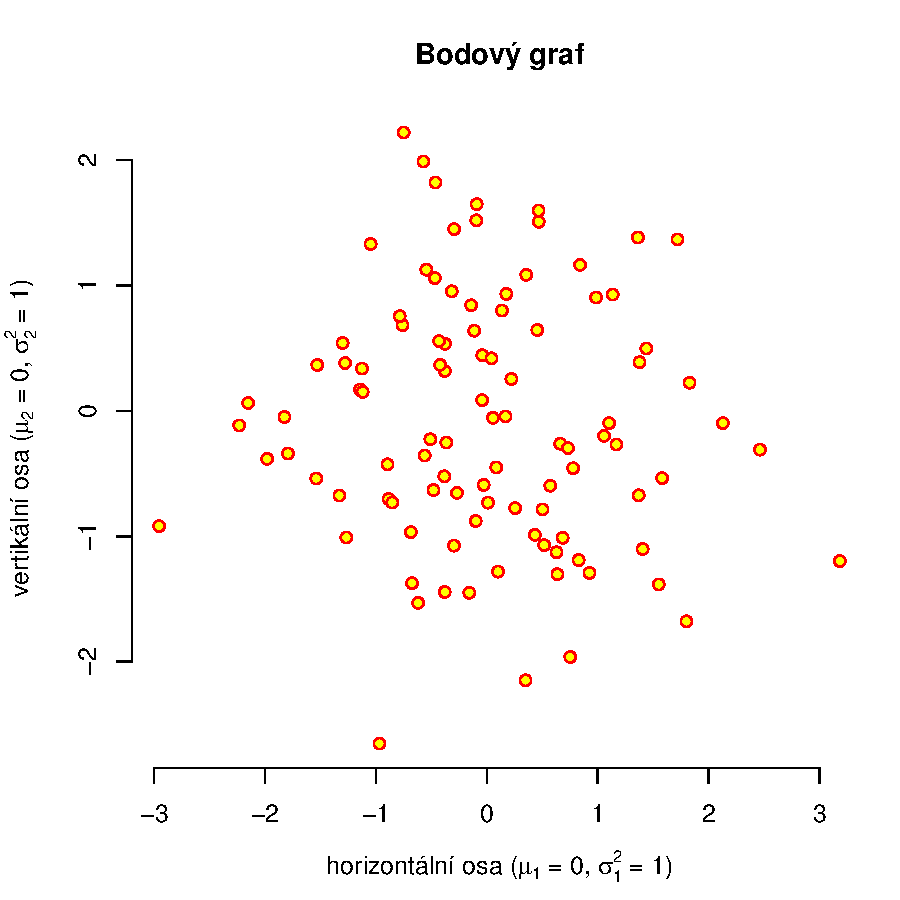
\includegraphics[width=140mm, height=140mm]{../img/ukazka-obr01}
% Příponu není potřeba explicitně uvádět, pdflatex automaticky hledá pdf.
% Rozměry také není nutné uvádět.
\caption{Náhodný výběr z~rozdělení $\mathcal{N}_2(\boldsymbol{0},\,I)$.}
\label{obr03:Nvyber}

\end{figure}

\begin{figure}[p]\centering
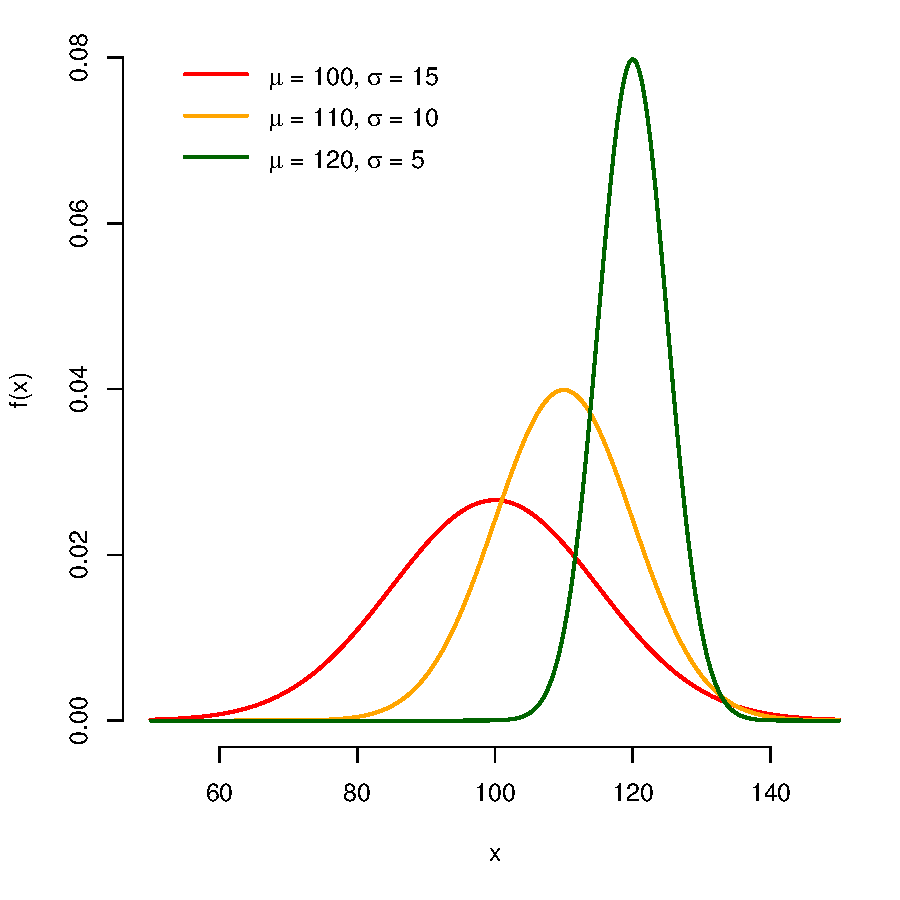
\includegraphics[width=140mm, height=140mm]{../img/ukazka-obr02}
\caption{Hustoty několika normálních rozdělení.}
\label{obr03:Nhust}
\end{figure}

\begin{figure}[p]\centering
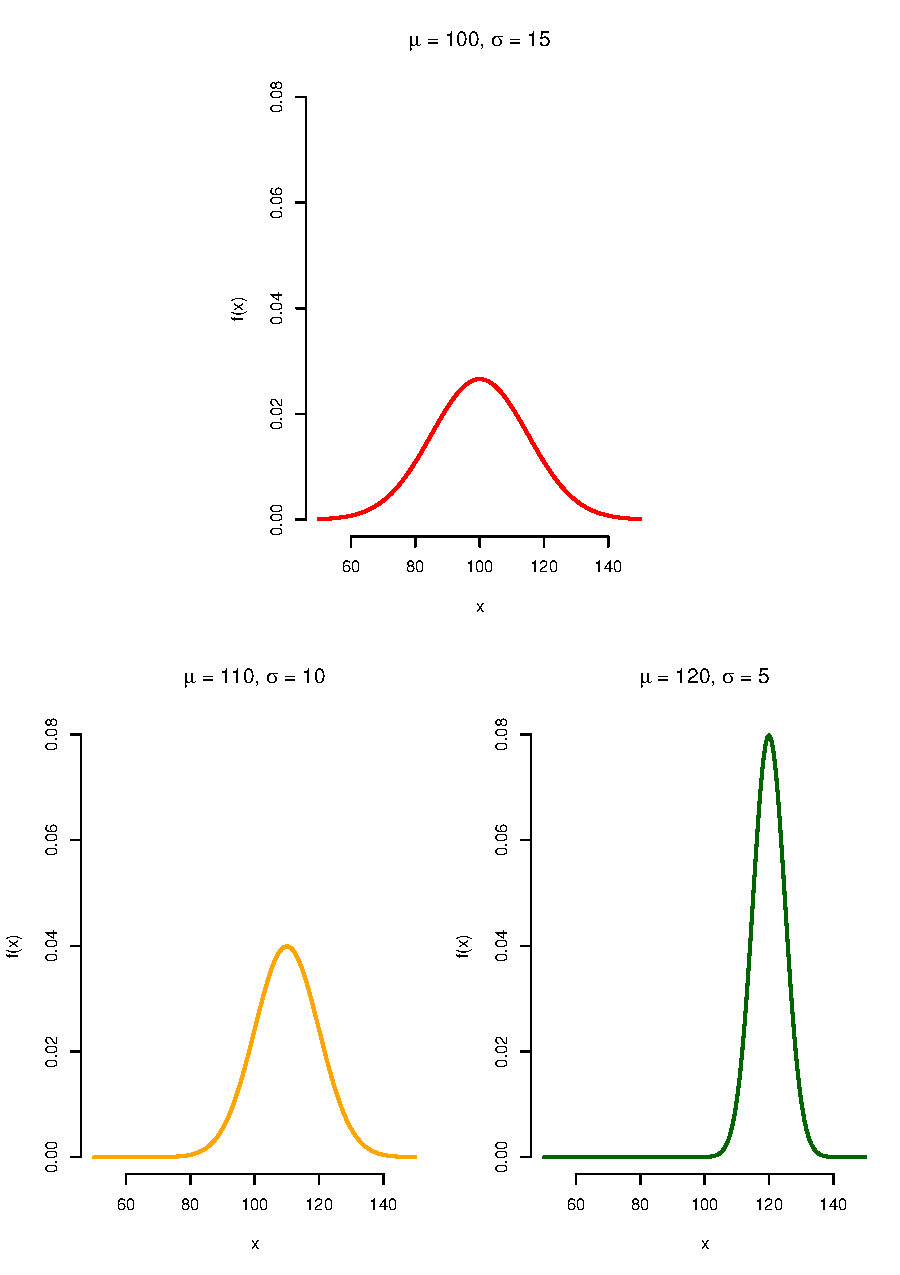
\includegraphics[width=140mm, height=198mm]{../img/ukazka-obr03}
\caption{Hustoty několika normálních rozdělení.}
\label{obr03:Nhust:podruhe}

\end{figure}

%!TEX root = ../prace.tex

\chapter{Uživatelská dokumentace}

\section{Požadavky pro spuštění hry}
\subsubsection{Hardwarové požadavky}

Doporučená minimální sestava (na ní byla hra vyvíjena): 

\begin{center}
	\begin{tabular} { | l | l |}
		\hline
		Procesor: 	&	Intel i7-2630QM @ 2.00GHz \\	\hline
		RAM:		&	12 GB	(8 GB by mělo také stačit) \\	\hline
		Grafika:	&	ATI Radeon HD 6700M \\	\hline
		OS:			&	Win 10 x64	(7 a~vyšší by měly též fungovat) \\
		\hline
	\end{tabular}
\end{center}

Výše uvedneou konfiguraci je potřeba brát jako orientační. Hru jsme úspěšně spustili i~na notebooku s~procesorem Intel i5, integrovanou grafickou kartou a~8 GB operační paměti. Bylo však nutné nastavit grafické vlastnosti na minimální možnou konfiguraci. 

\subsubsection{Softwarové požadavky}

Pro spuštění zkompilované hry není potřeba nic speciálního. Je zapotřebí mít stroj s~minimální uvedenou konfigurací. Dále je dobré mít nainstalované poslední verze ovladačů HW komponent (hlavně grafiky). Taktéž je zapotřebí mít nainstalovanou poslední verzi DirectX a~C++ runtime. Tyto části lze doinstalovat z~přiloženého DVD ze složky \textit{Redist}.


\section{Tutoriál}
Tato hra obsahuje pokročilý tutoriál, ve kterém se lze snadno naučit veškeré principy hry. Ten je dostupný z~dialogu výběru nové hry. Proto se nebudeme zabývat podrobným popisem uživatelské dokumentace.
\begin{figure}[!ht]\centering
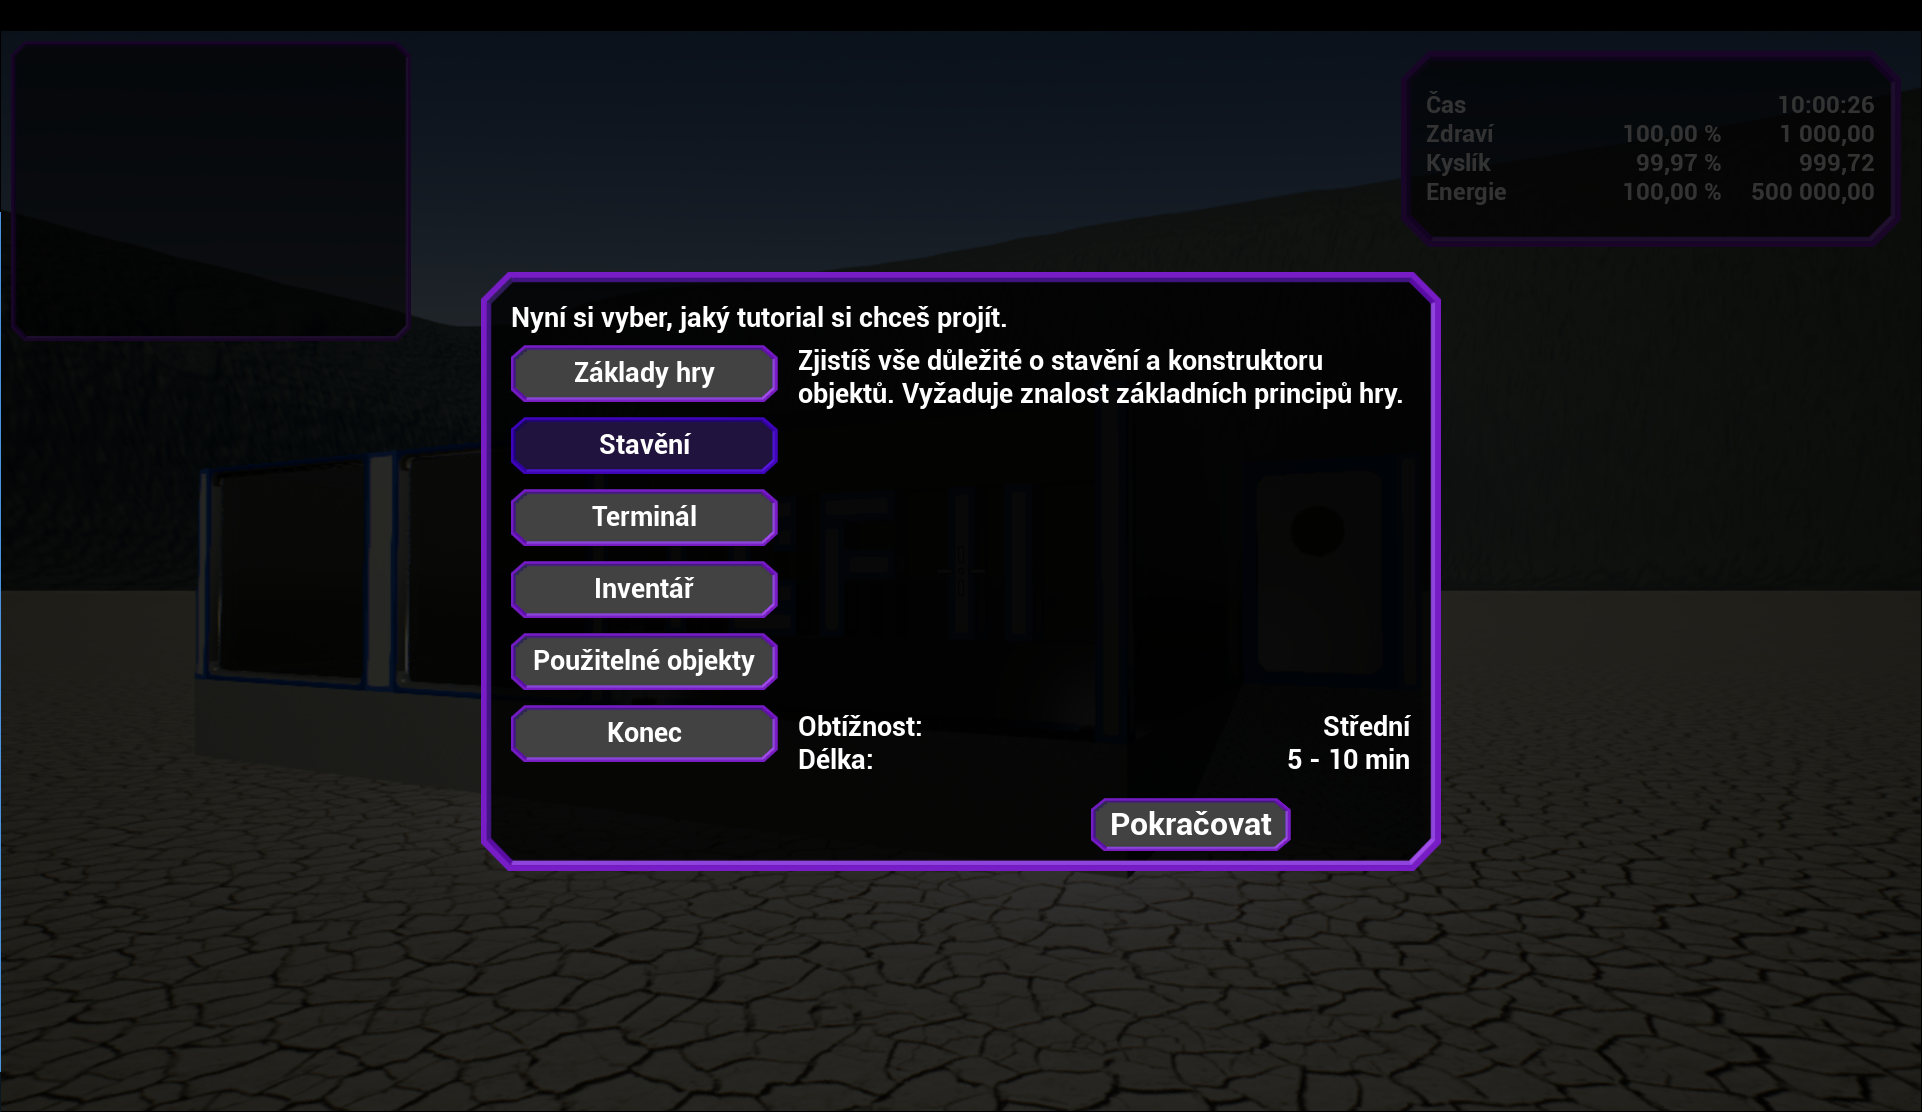
\includegraphics[ width=140mm]{../img/user/mainMenu/mmTut}

\caption{Výběr herního tutoriálu}
\label{fig:usr_tut}

\end{figure}
\FloatBarrier


%!TEX root = ../../prace.tex

\section{Hlavní menu}

Po načtení hry hráč vidí hlavní menu. Denní doba i~počasí se zvolí náhodně.

\begin{figure}[!ht]\centering
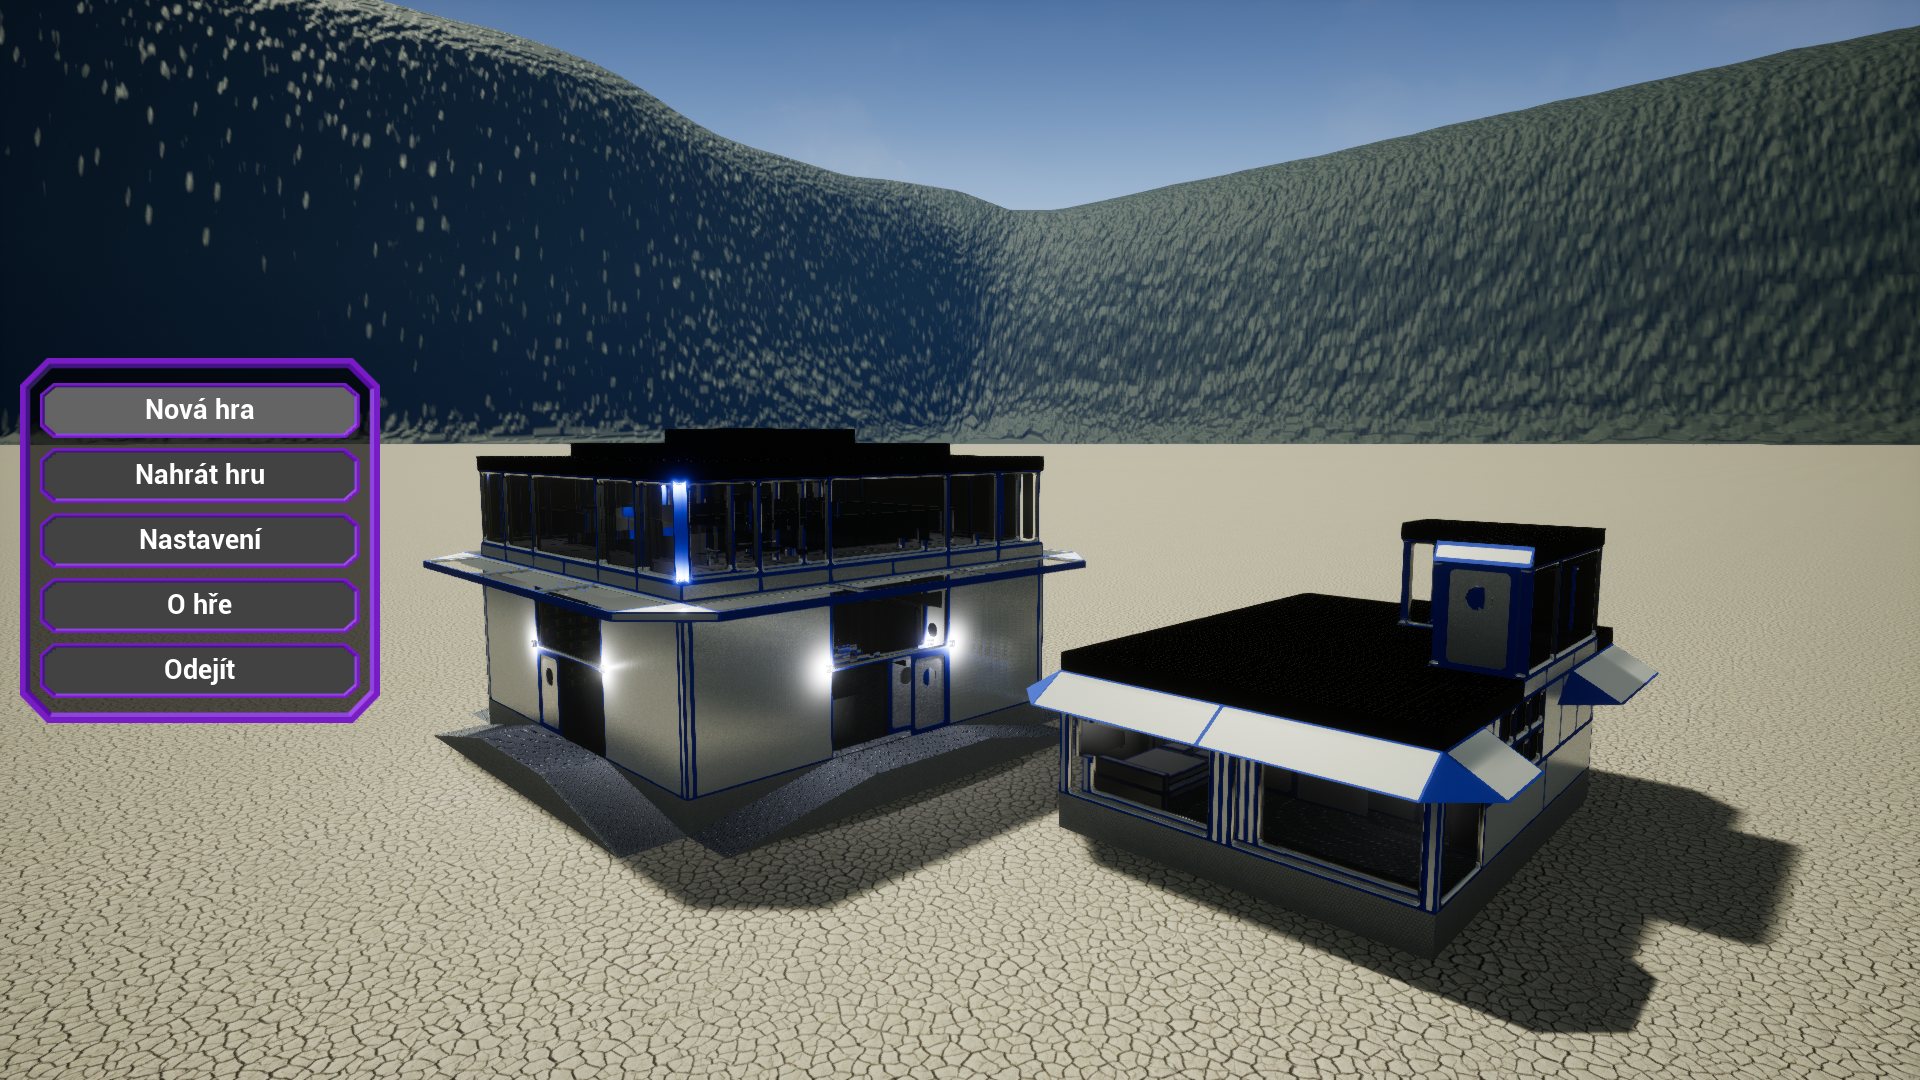
\includegraphics[ width=140mm]{../img/user/mainMenu/mmDay}

\caption{Obrazovka hlavního menu -- den}
\label{fig:user_mainMenu_mmDay}

\end{figure}


\FloatBarrier

První volba, kterou je možné zvolit, je výběr nové hry. K~dispozici je několik variant s~různými obtížnostmi.

\begin{figure}[!ht]\centering
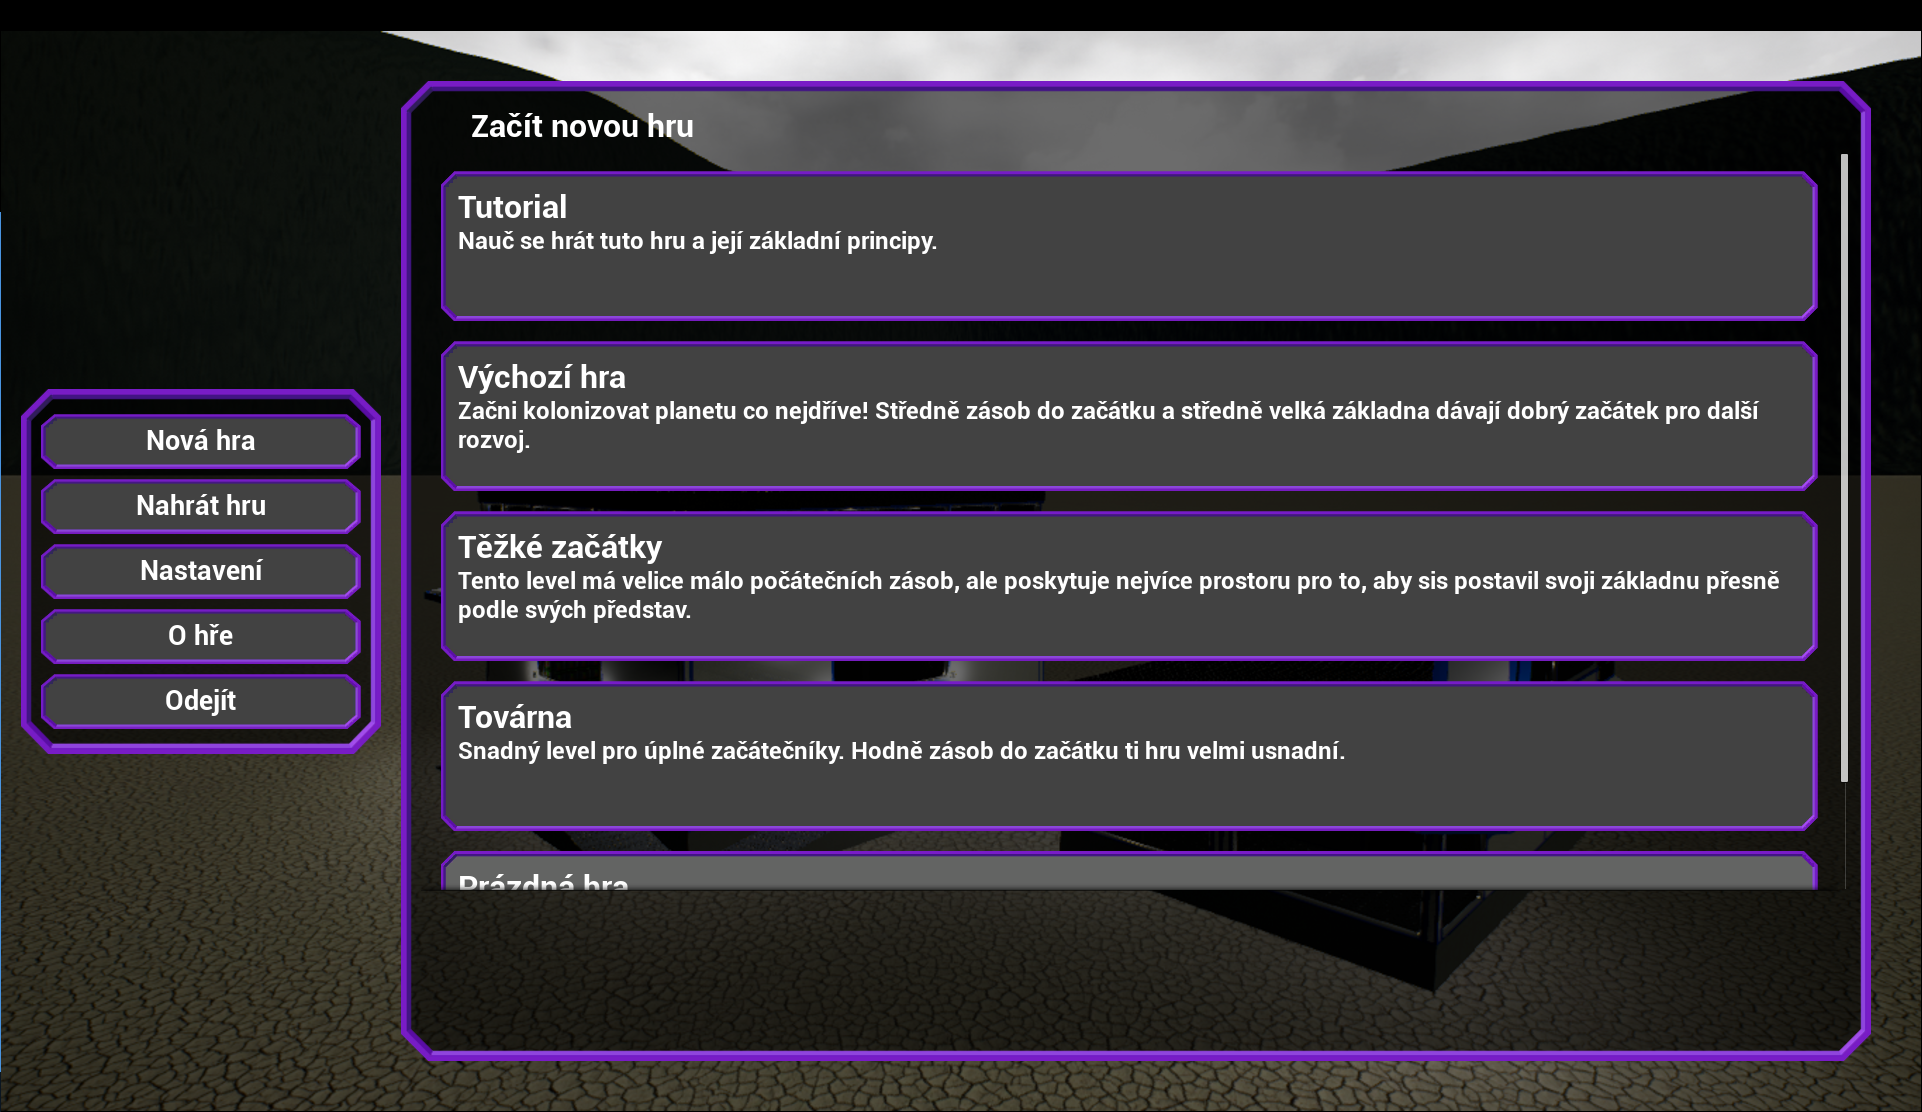
\includegraphics[ width=140mm]{../img/user/mainMenu/mmBegin}

\caption{Obrazovka hlavního menu -- Nová hra}
\label{fig:user_mainMenu_mmBegin}

\end{figure}
\FloatBarrier

Pokud hráč má nějaké uložené hry, může si je nahrát kliknutím na tlačítko \textbf{Nahrát hru}. V~tomto případě žádné uložené hry k~načtení k~dispozici nejsou.

\begin{figure}[!ht]\centering
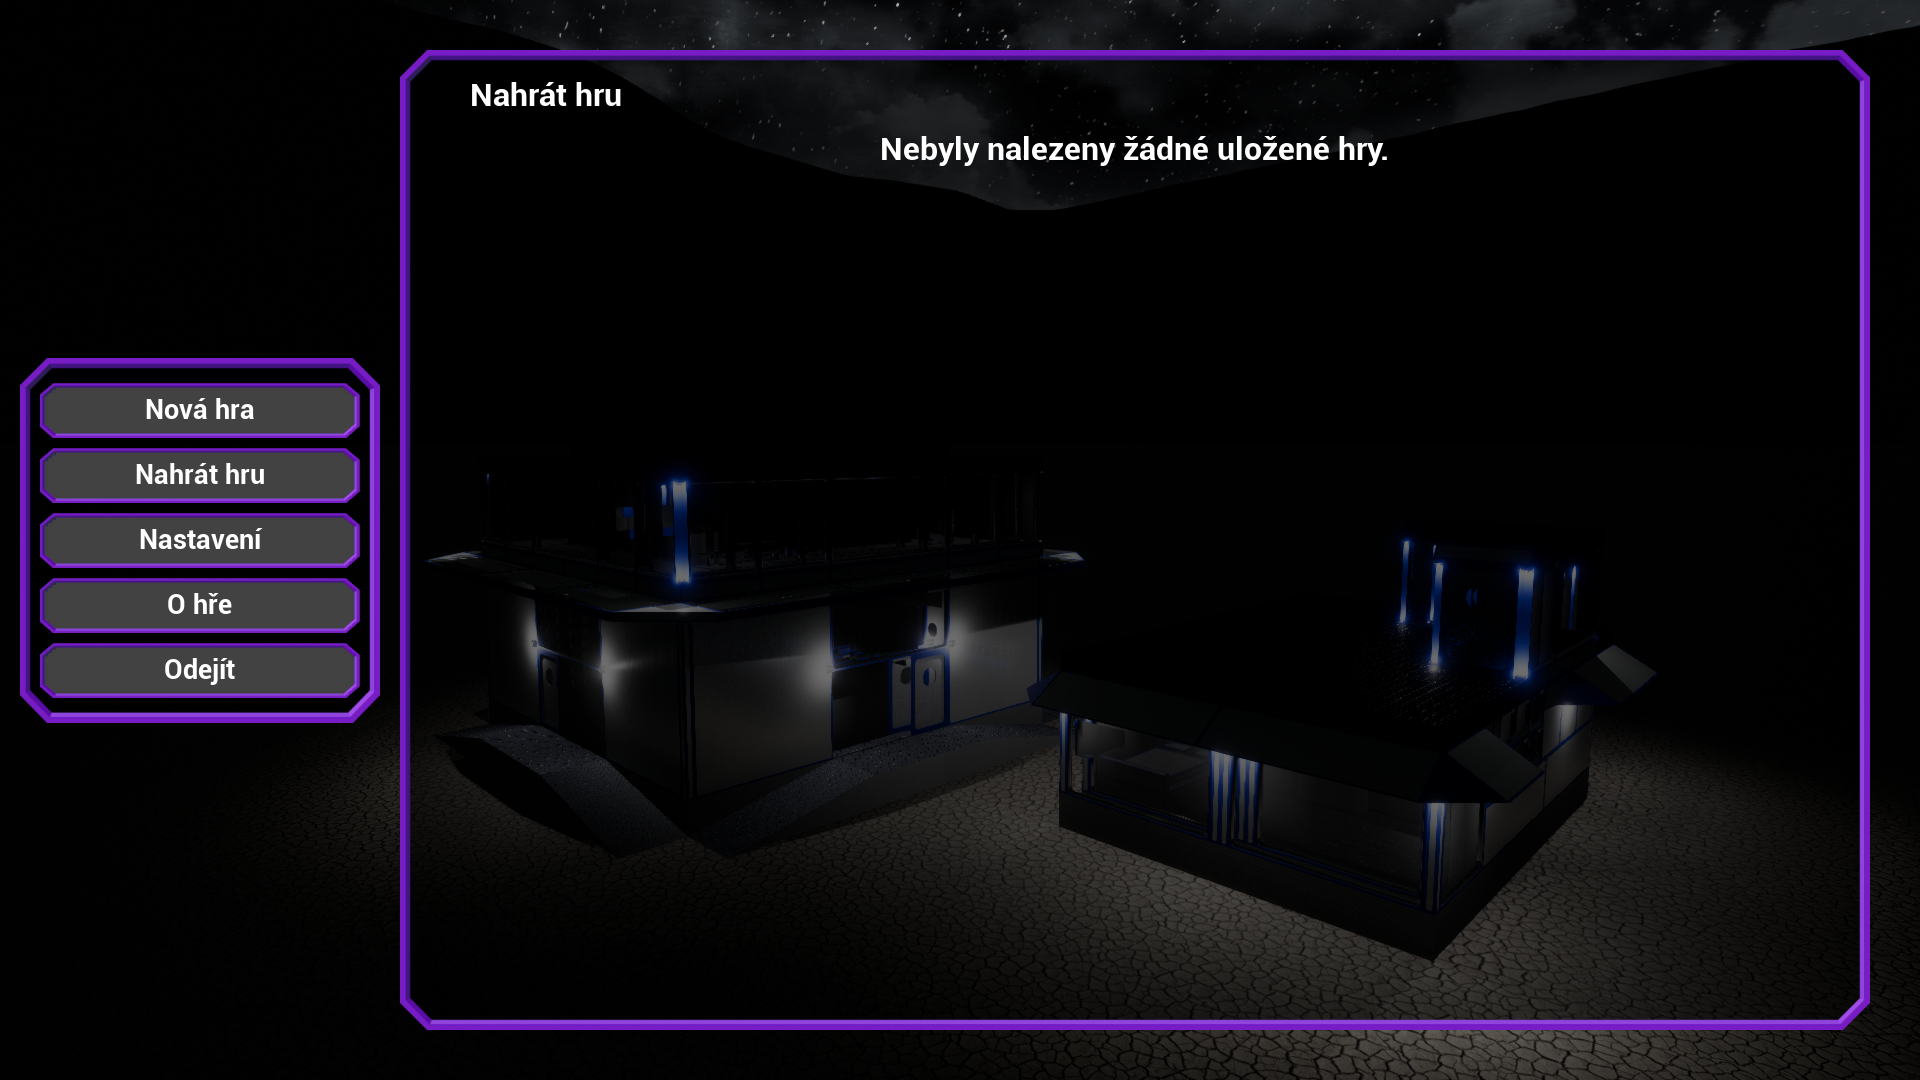
\includegraphics[ width=140mm]{../img/user/mainMenu/mmLoad}

\caption{Obrazovka hlavního menu -- Nahrát hru}
\label{fig:user_mainMenu_mmLoad}

\end{figure}
\FloatBarrier

Pod položkou \textbf{Nastavení} může uživatel měnit herní, zvuková a~grafická nastavení hry. Nastavení se aplikují a~ukládají okamžitě, výjimkou je pouze položka \textit{Animace generátoru energie}, která se projeví až po změně levelu. V~případě konfigurace z~hlavní nabídky se nastavení projeví okamžitě, v~případě konfigurace během rozehrané hry je potřeba vyvolat opětovné načtení uložené hry, nebo znovu spustit novou hru.

\begin{figure}[!ht]\centering
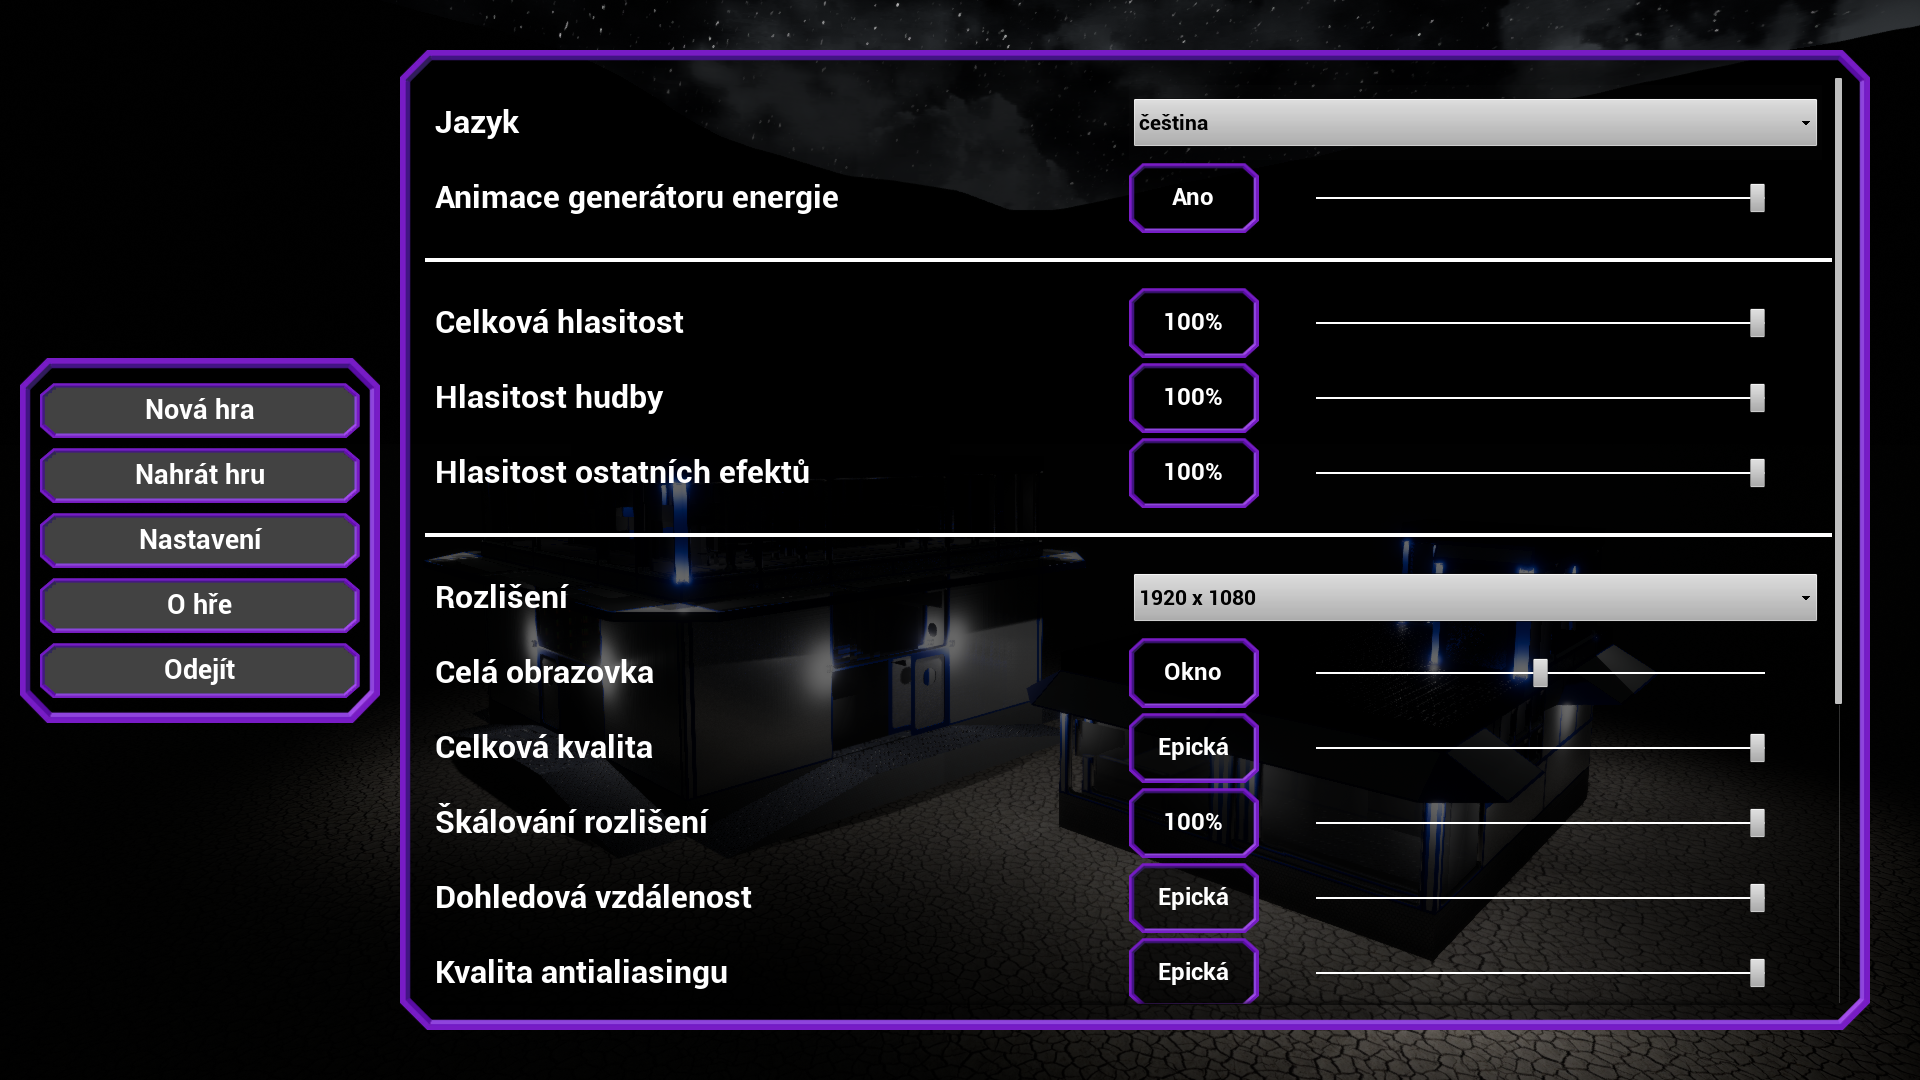
\includegraphics[ width=140mm]{../img/user/mainMenu/mmSettings}

\caption{Obrazovka hlavního menu -- Nastavení}
\label{fig:user_mainMenu_mmSettings}

\end{figure}

\FloatBarrier
%!TEX root = ../../prace.tex

\section{Herní menu - ukládání, nahrávání}

V průběhu rozehrané hry je možné použít \textbf{Rychlé uložení / načtení}, nebo si hru uložit z~herní nabídky.

Pro uložení hry je možné vytvořit nový save nebo přepsat stávající, pokud nějaký existuje. Uložené hry je též možné mazat.

\begin{figure}[!ht]\centering
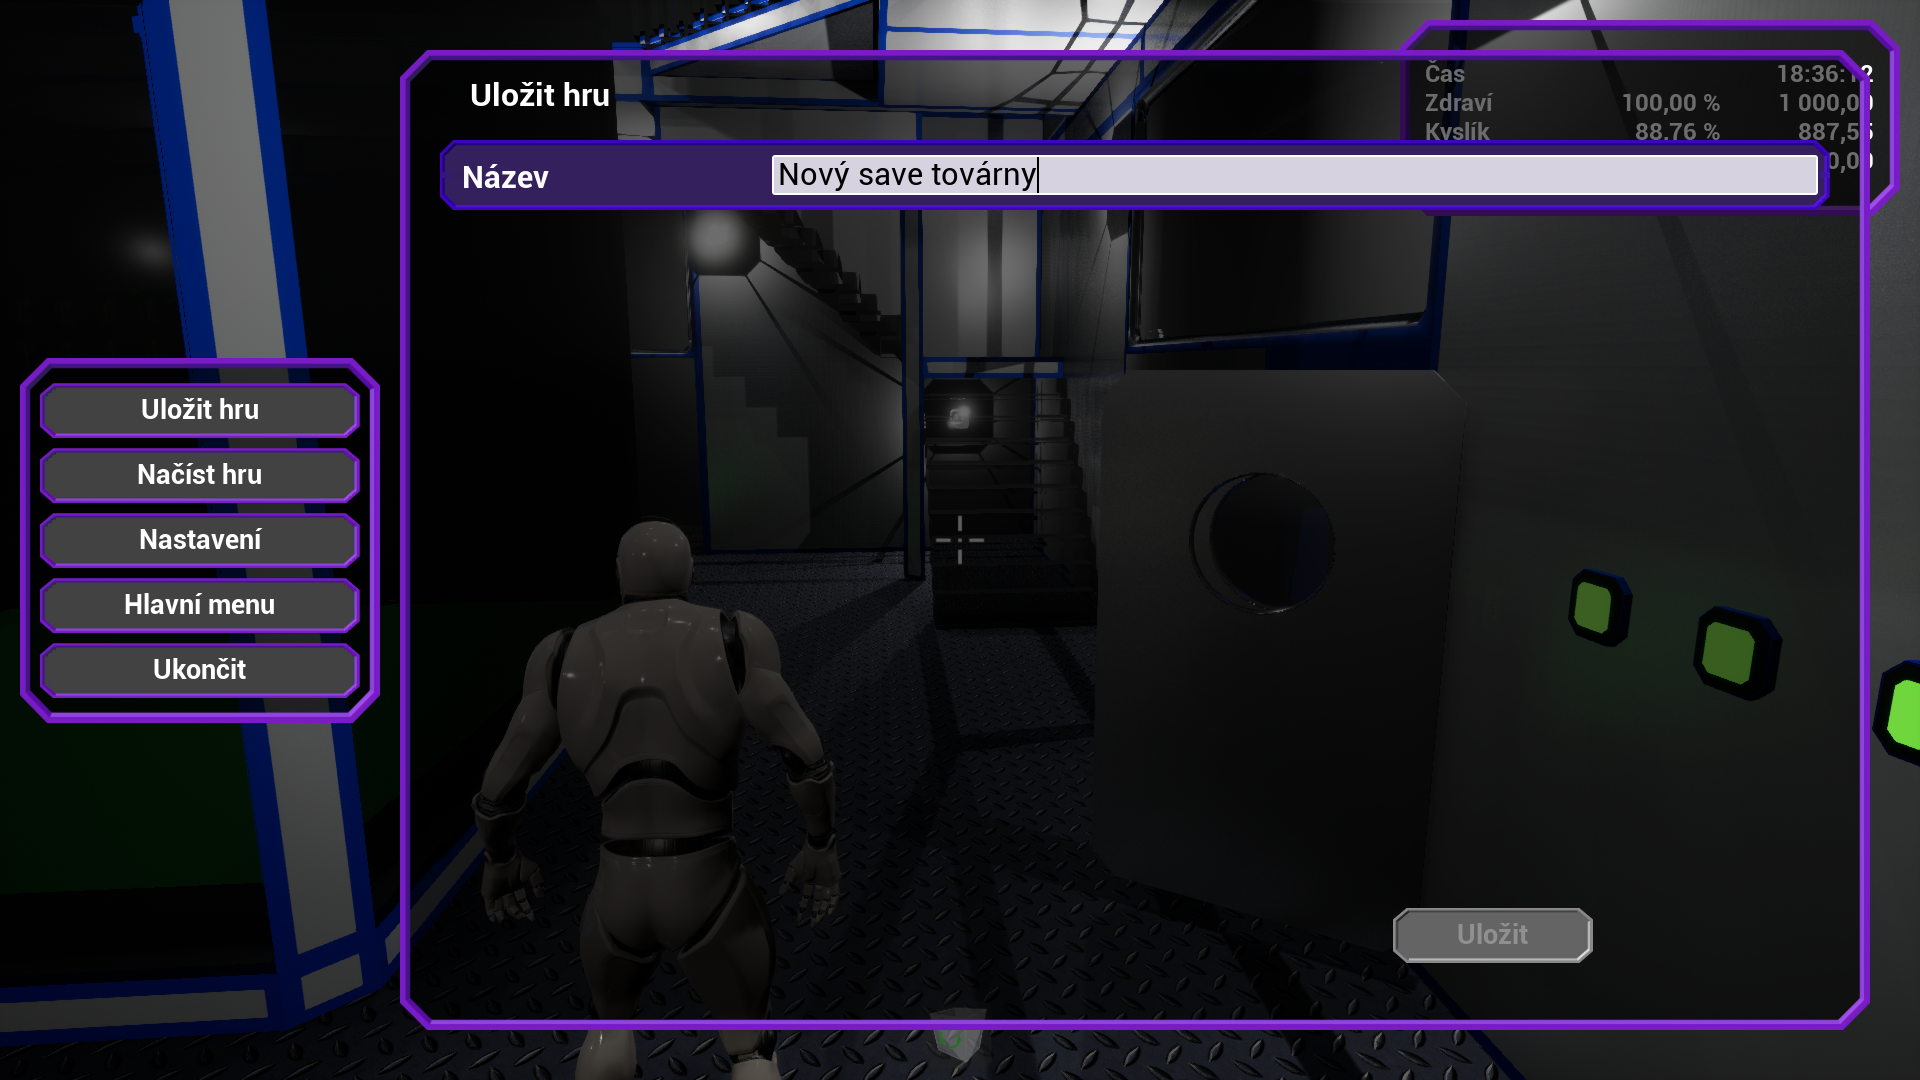
\includegraphics[ width=140mm]{../img/user/save/0newSave}

\caption{Ukládání - Nový save}
\label{fig:user_save_0newSave}

\end{figure}
\FloatBarrier

Pokud bylo uložení úspěšné, hráči se zobrazí následující hláška:

\begin{figure}[!ht]\centering
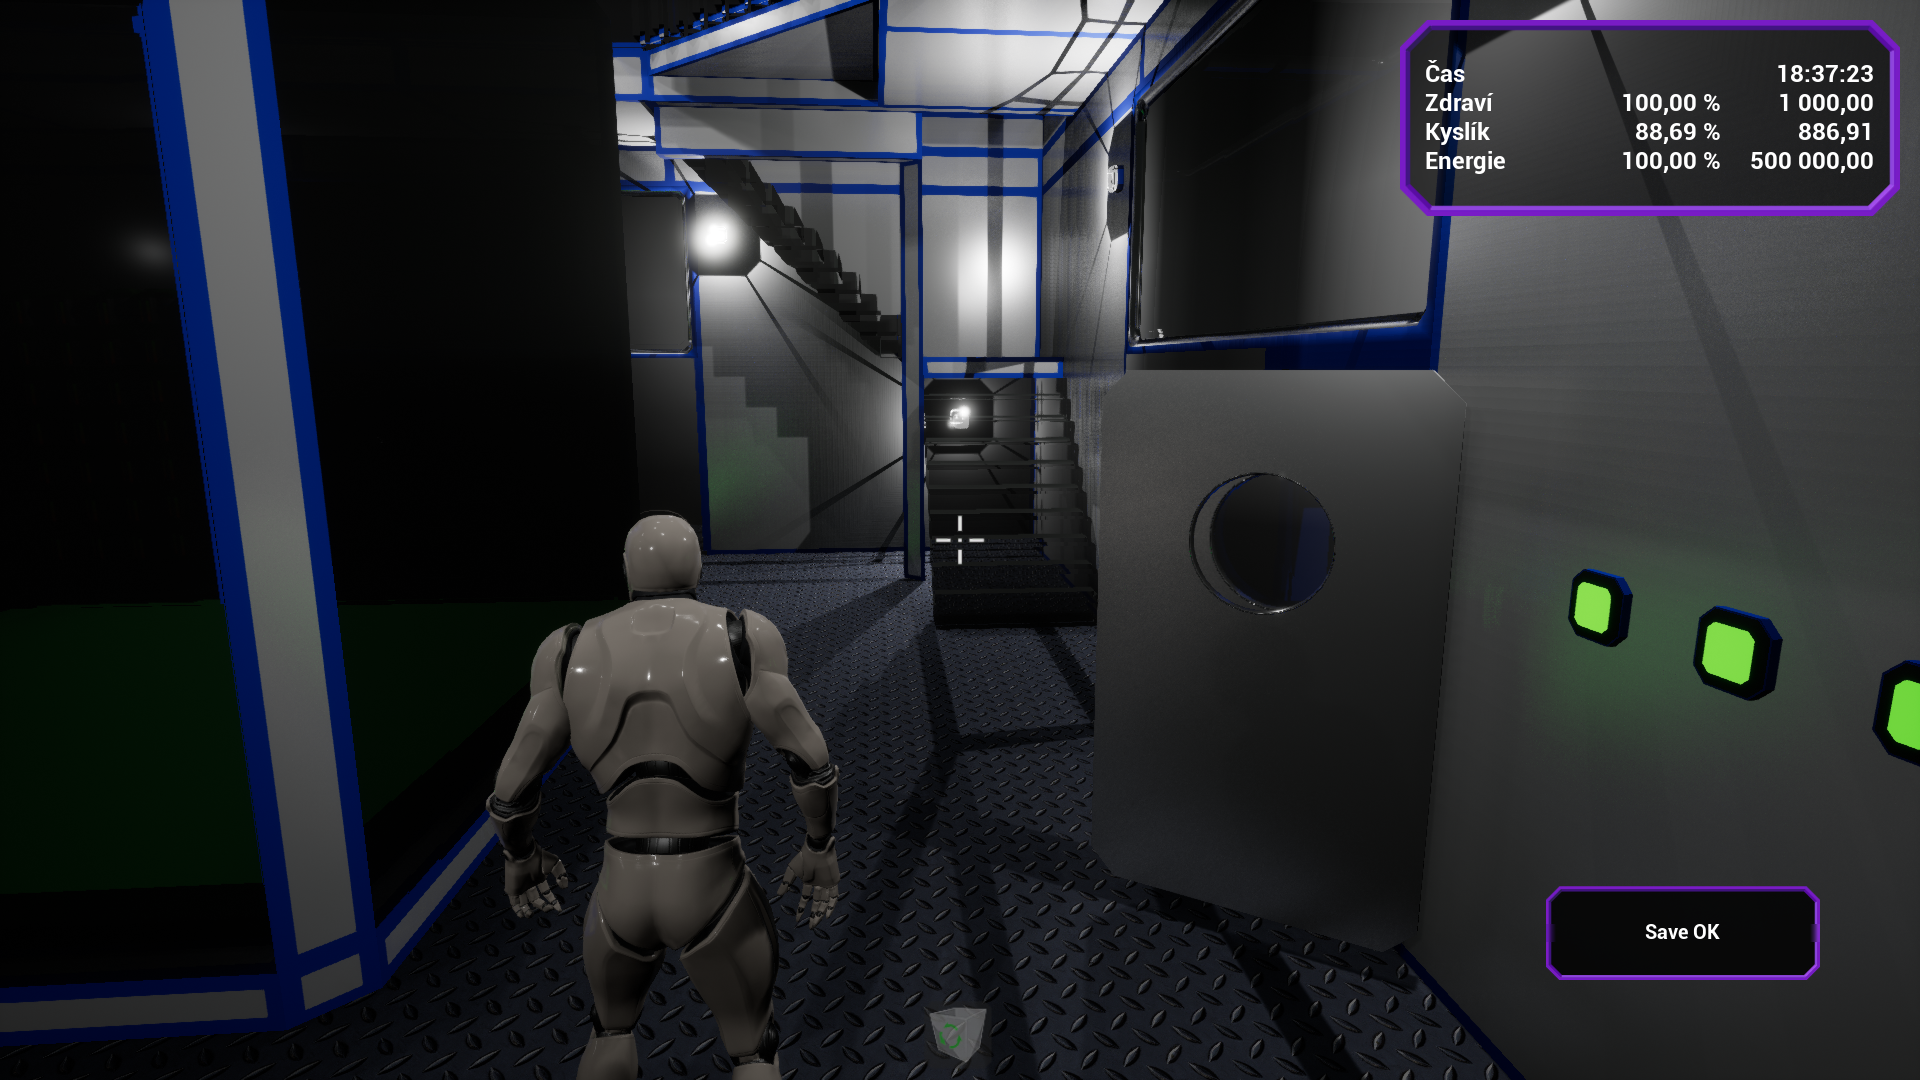
\includegraphics[ width=140mm]{../img/user/save/1afterSave}

\caption{Ukládání - po uložení}
\label{fig:user_save_1afterSave}

\end{figure}
\FloatBarrier

Nahrávat je možné ze všech uložených pozic, včetně rychlého uložení. Opět je zde možné vybraný save smazat.

\begin{figure}[!ht]\centering
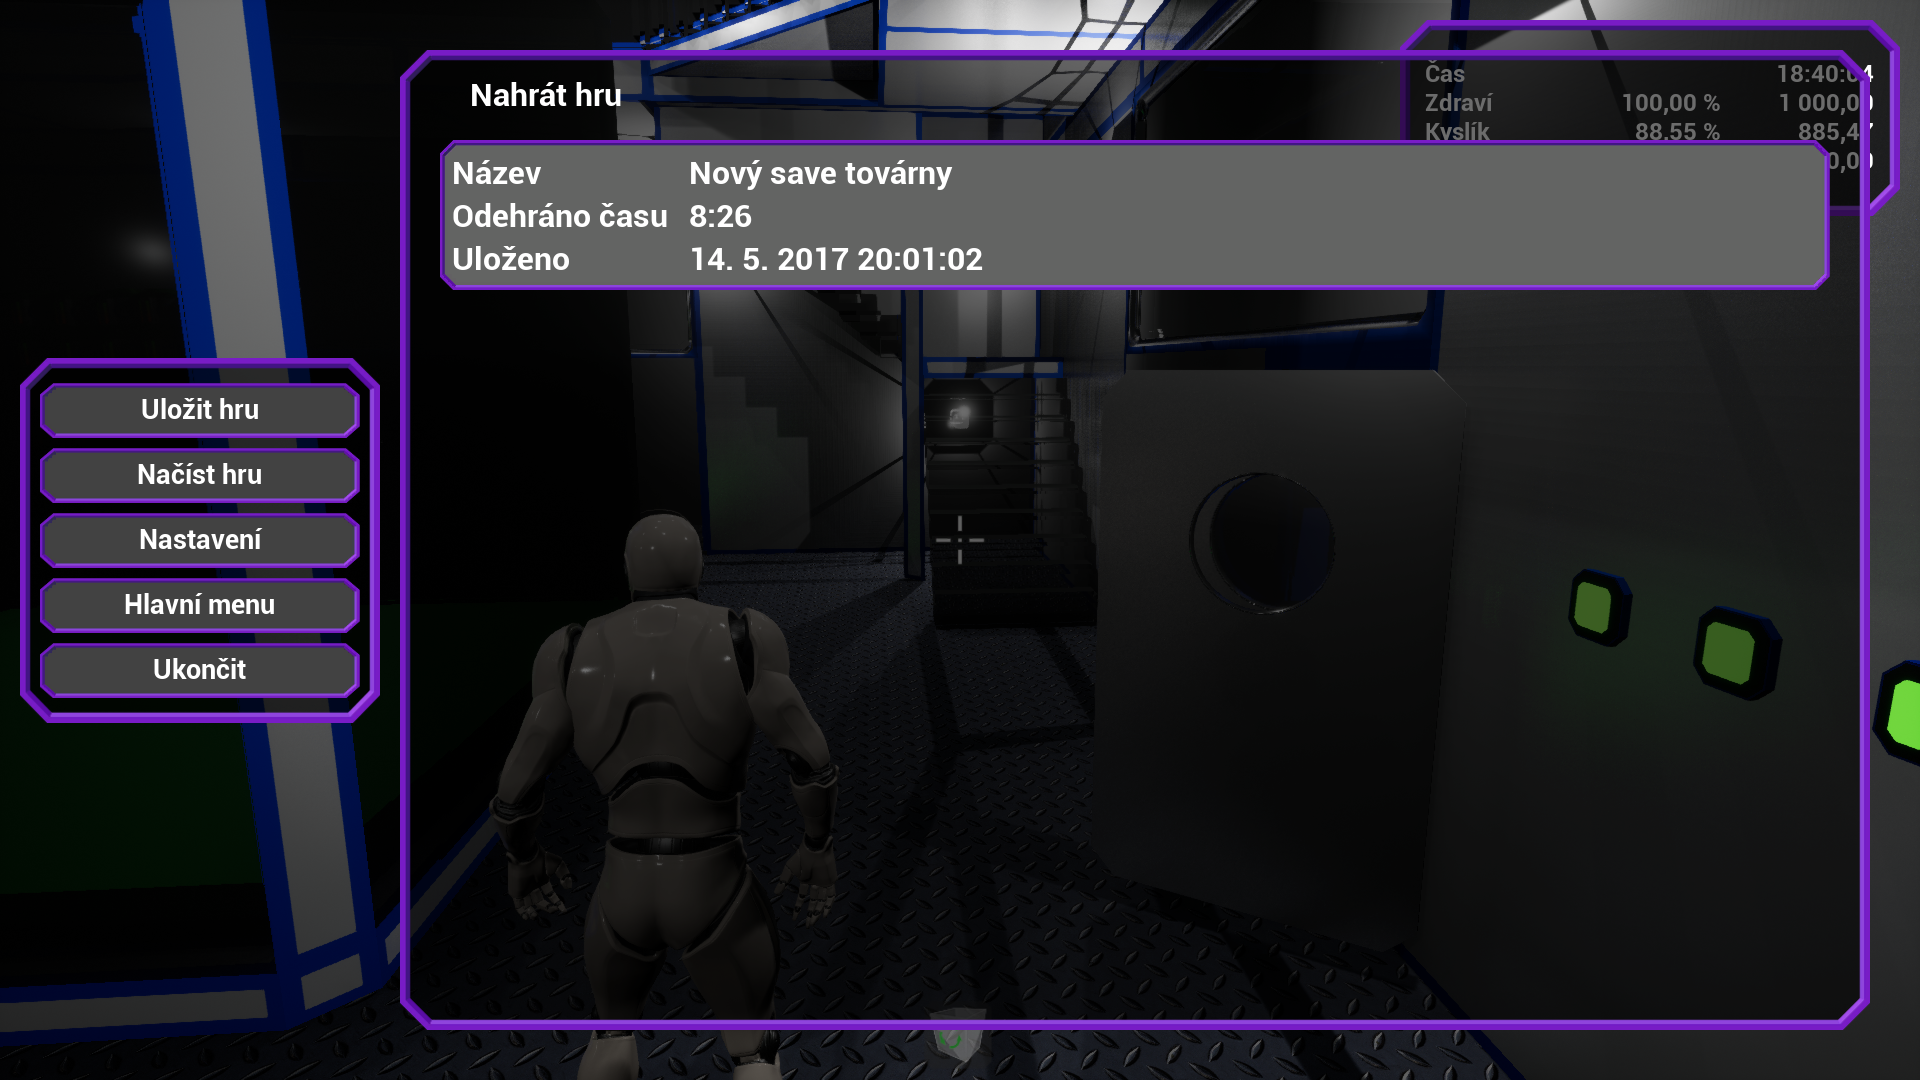
\includegraphics[ width=140mm]{../img/user/save/2load}

\caption{Ukládání - nahrát hru}
\label{fig:user_save_2load}

\end{figure}
\FloatBarrier

Pokud má hráč rozehranou hru, je pro jistotu vyžadováno potvrzení.

\begin{figure}[!ht]\centering
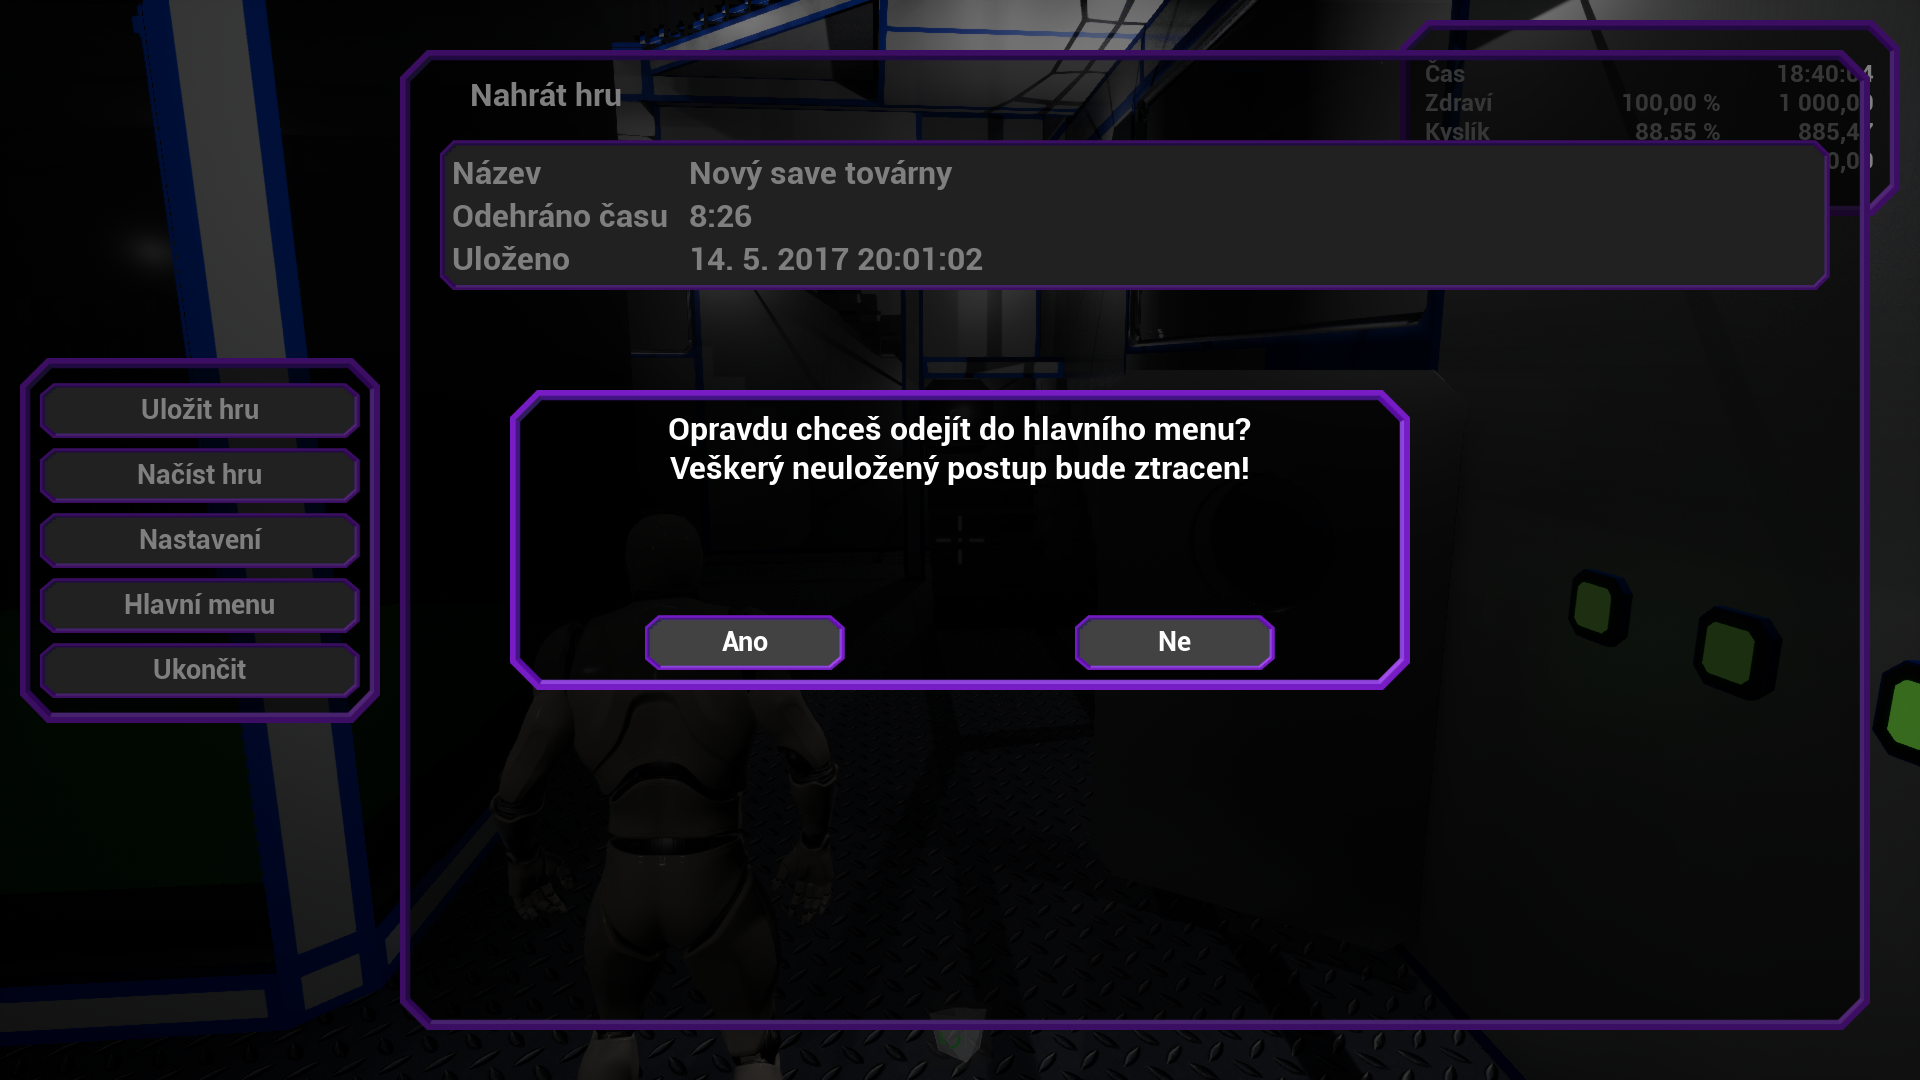
\includegraphics[ width=140mm]{../img/user/save/3loadClicked}

\caption{Ukládání - potvrzení nahrání hry}
\label{fig:user_save_3loadClicked}

\end{figure}

\FloatBarrier
%!TEX root = ../../prace.tex

\section{Inventář}

Inventář se vyvolá klávesou \textbf{E}. Zobrazí se následující obrazovka:

\begin{figure}[!ht]\centering
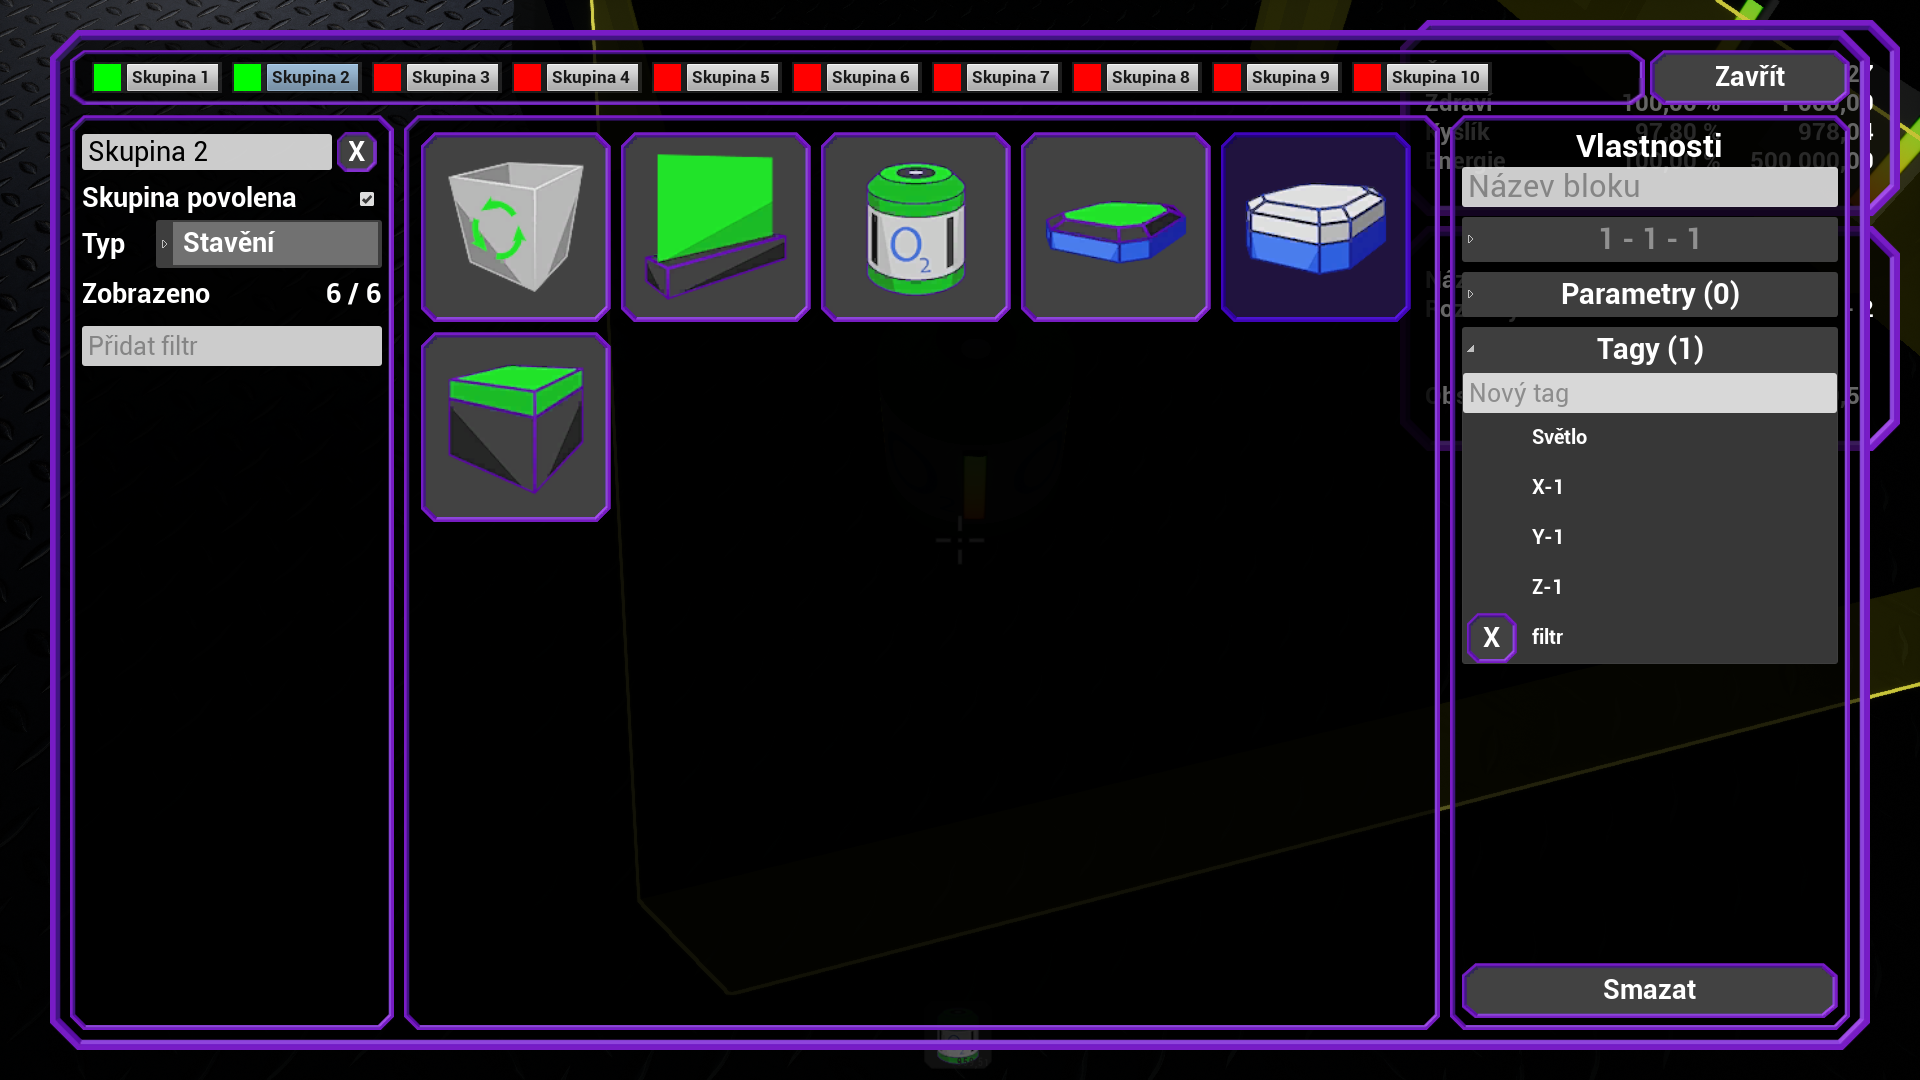
\includegraphics[ width=140mm]{../img/user/inventory/0AddTag}

\caption{Inventář - přehled}
\label{fig:user_inventory_0AddTag}

\end{figure}

\FloatBarrier

V horní části je výběr skupin. Je možné vybírat z 10 skupin, které si lze pojmenovat dle libosti. Dále je možné je (de)aktivovat buď kliknutím na zelený / červený čtverec, nebo skrze příslušný checkbox v editaci skupiny.
Je možné používat standardní změnu skupiny klávesami \textbf{ú} a \textbf{)}, editační okno se pak příslušným způsobem změní. 

V \textit{levé} části je \textbf{editor skupiny}, jehož funkce budou popsány v textu dále. \textit{Uprostřed} je možné vidět postavitelné či umístitelné položky, které jsou dofiltrovány dle právě nastaveného filtru. Výběrem položky lze editovat její vlastnosti v \textit{pravé} části okna

\FloatBarrier

Každá skupina umožňuje definovat své filtry. Matematicky bychom mohli popsat filtrování jako vyhodnocení formule v \textit{CNF}. Pokud do pole \textit{Přidat filtr} napíšeme tagy oddělené mezerou, do skupiny se přidá \textbf{nová} skupina s výchozím pojmenováním.

\begin{figure}[!ht]\centering
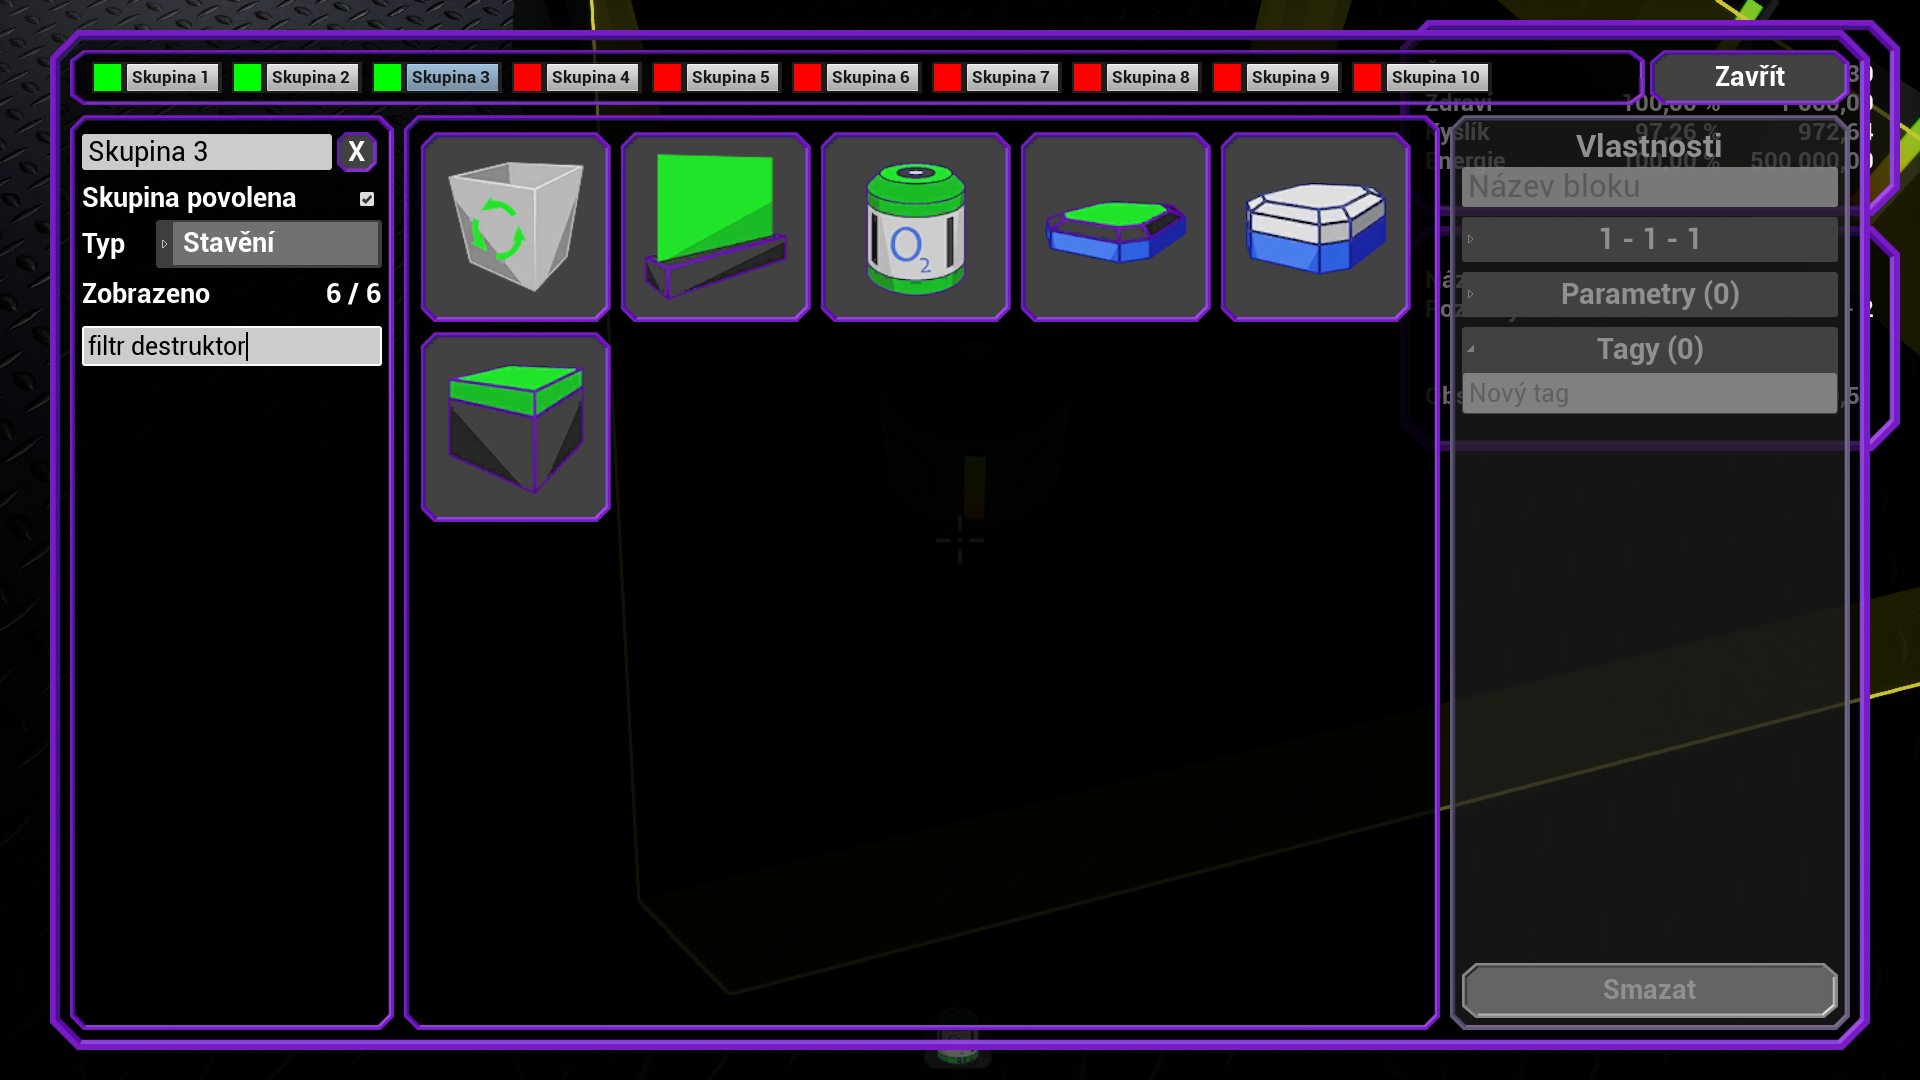
\includegraphics[ width=140mm]{../img/user/inventory/1setFilter}

\caption{Inventář - přidání skupiny}
\label{fig:user_inventory_1setFilter}

\end{figure}

\FloatBarrier

Po přidání se seznam dostupných prvků dofiltruje podle nastavených tagů - ve výsledku bude každá položka splňovat alespoň jeden tag z každé skupiny. Shoda nemusí být přesná, tag objektu musí obsahovat podřetězec definovaný filtrem.
\begin{figure}[!ht]\centering
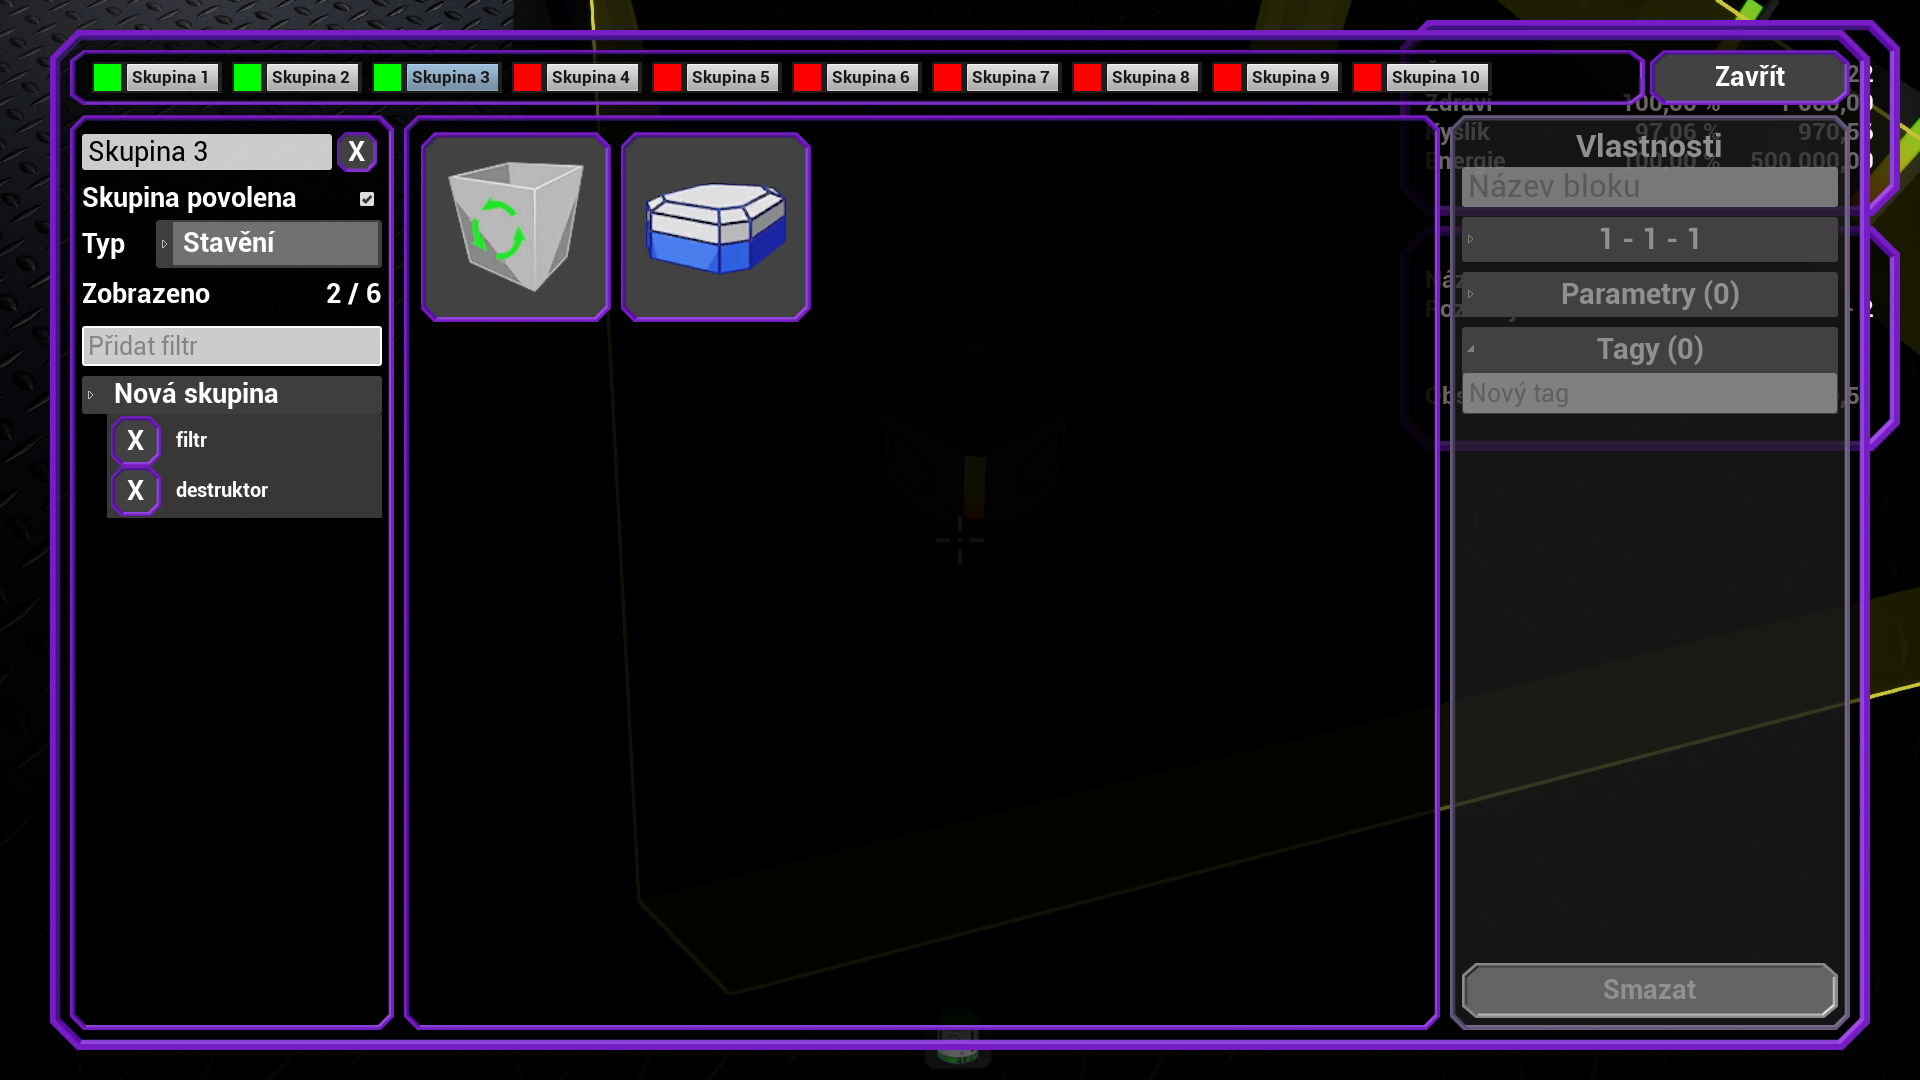
\includegraphics[ width=140mm]{../img/user/inventory/2filterResult}

\caption{Inventář - výsledek s filtrovanými položkami}
\label{fig:user_inventory_2filterResult}

\end{figure}

\FloatBarrier

Na následujícím obrázku je možné vidět filtry s rozbalenými vlastnostmi. Zaměřme se nyní na část \textit{Nesbalovat}. Po zaškrtnutí této volby je zobrazena pouze hlavička skupiny.

\begin{figure}[!ht]\centering
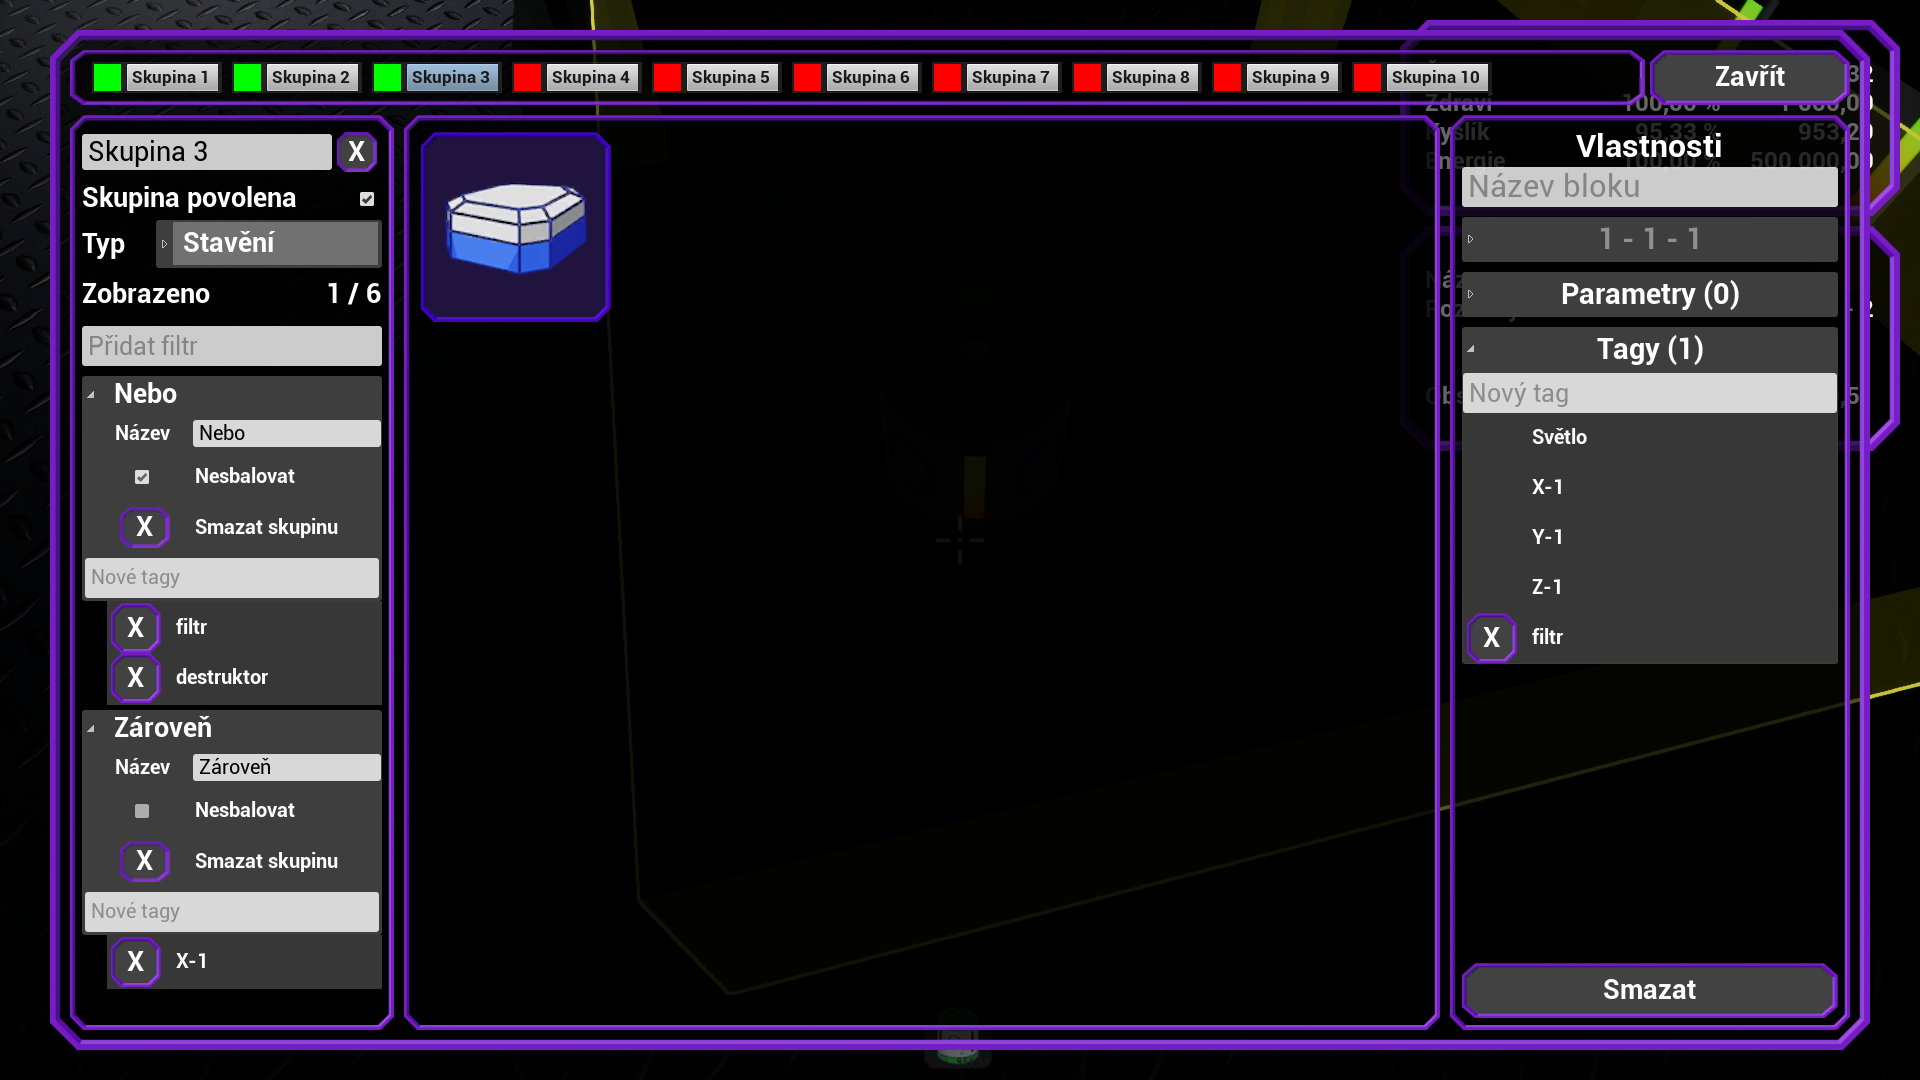
\includegraphics[ width=140mm]{../img/user/inventory/3additionalFilter}

\caption{Inventář - Nová hra}
\label{fig:user_inventory_3additionalFilter}

\end{figure}

\FloatBarrier

Výsledný seznam se sbalenými vlastnostmi filtru:

\begin{figure}[!ht]\centering
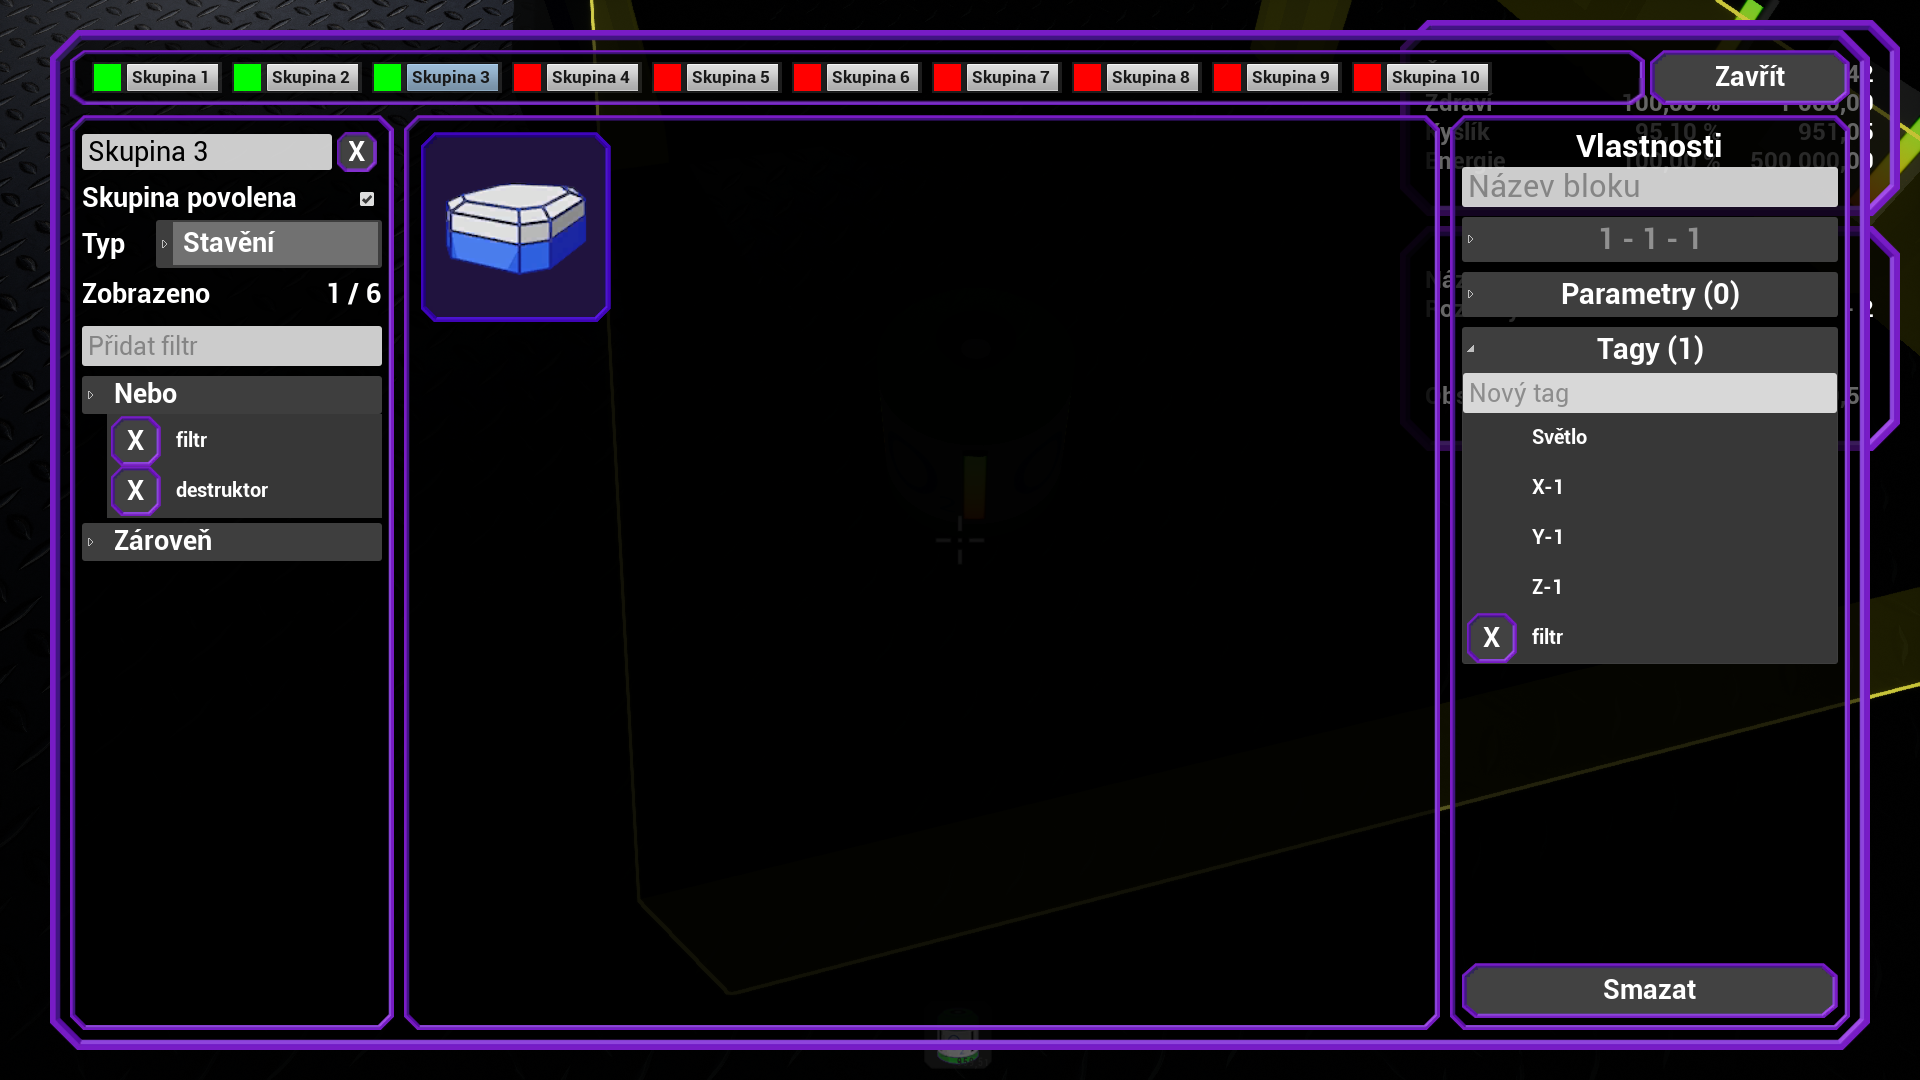
\includegraphics[ width=140mm]{../img/user/inventory/4addFilterCollapsed}

\caption{Inventář - Nahrát hru}
\label{fig:user_inventory_4addFilterCollapsed}

\end{figure}

\FloatBarrier

Označené položky je také možné smazat z inventáře. Umístitelné položky tak mohou být reálně zničeny. 

\begin{figure}[!ht]\centering
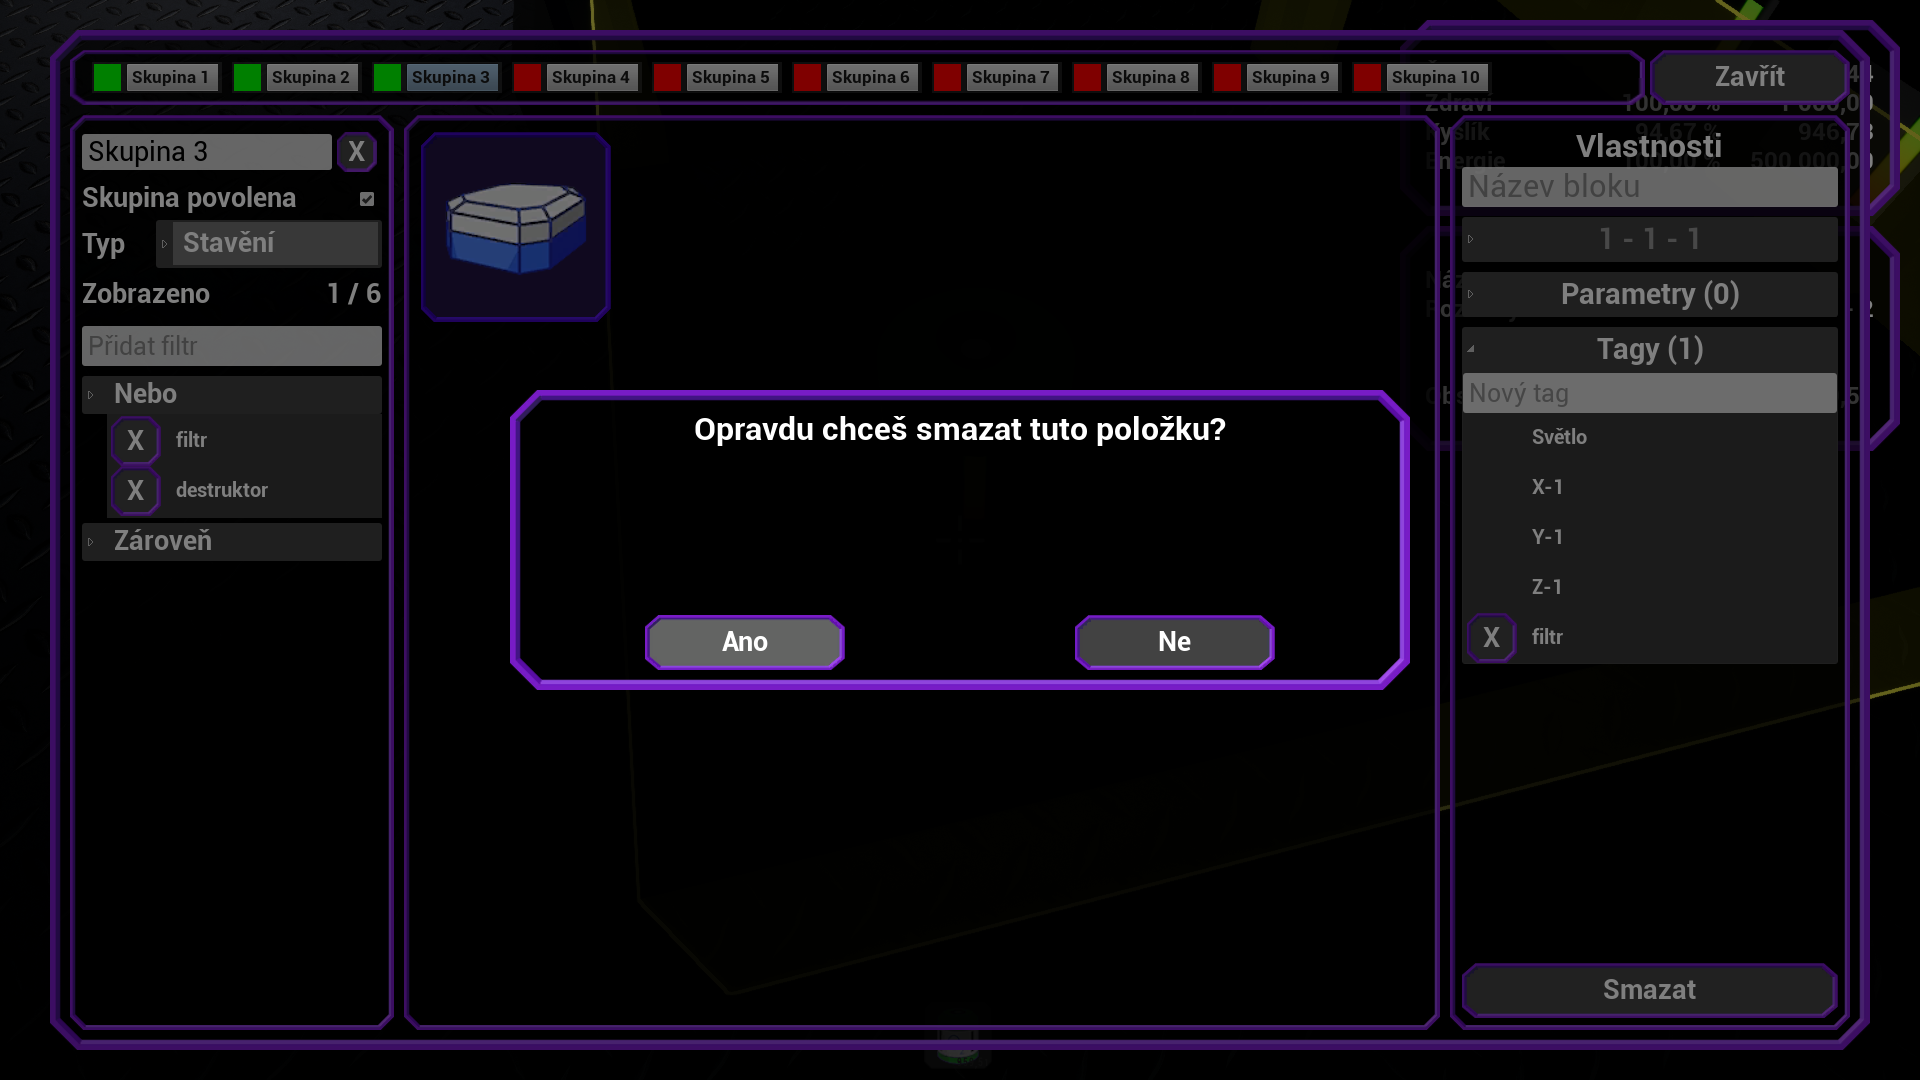
\includegraphics[ width=140mm]{../img/user/inventory/5deleteItem}

\caption{Inventář - Nastavení}
\label{fig:user_inventory_5deleteItem}

\end{figure}

\FloatBarrier
V případě, že je zvolena položka s dodatečnými parametry, je možné jejich hodnoty vidět v editoru vlastností bloku

\begin{figure}[!ht]\centering
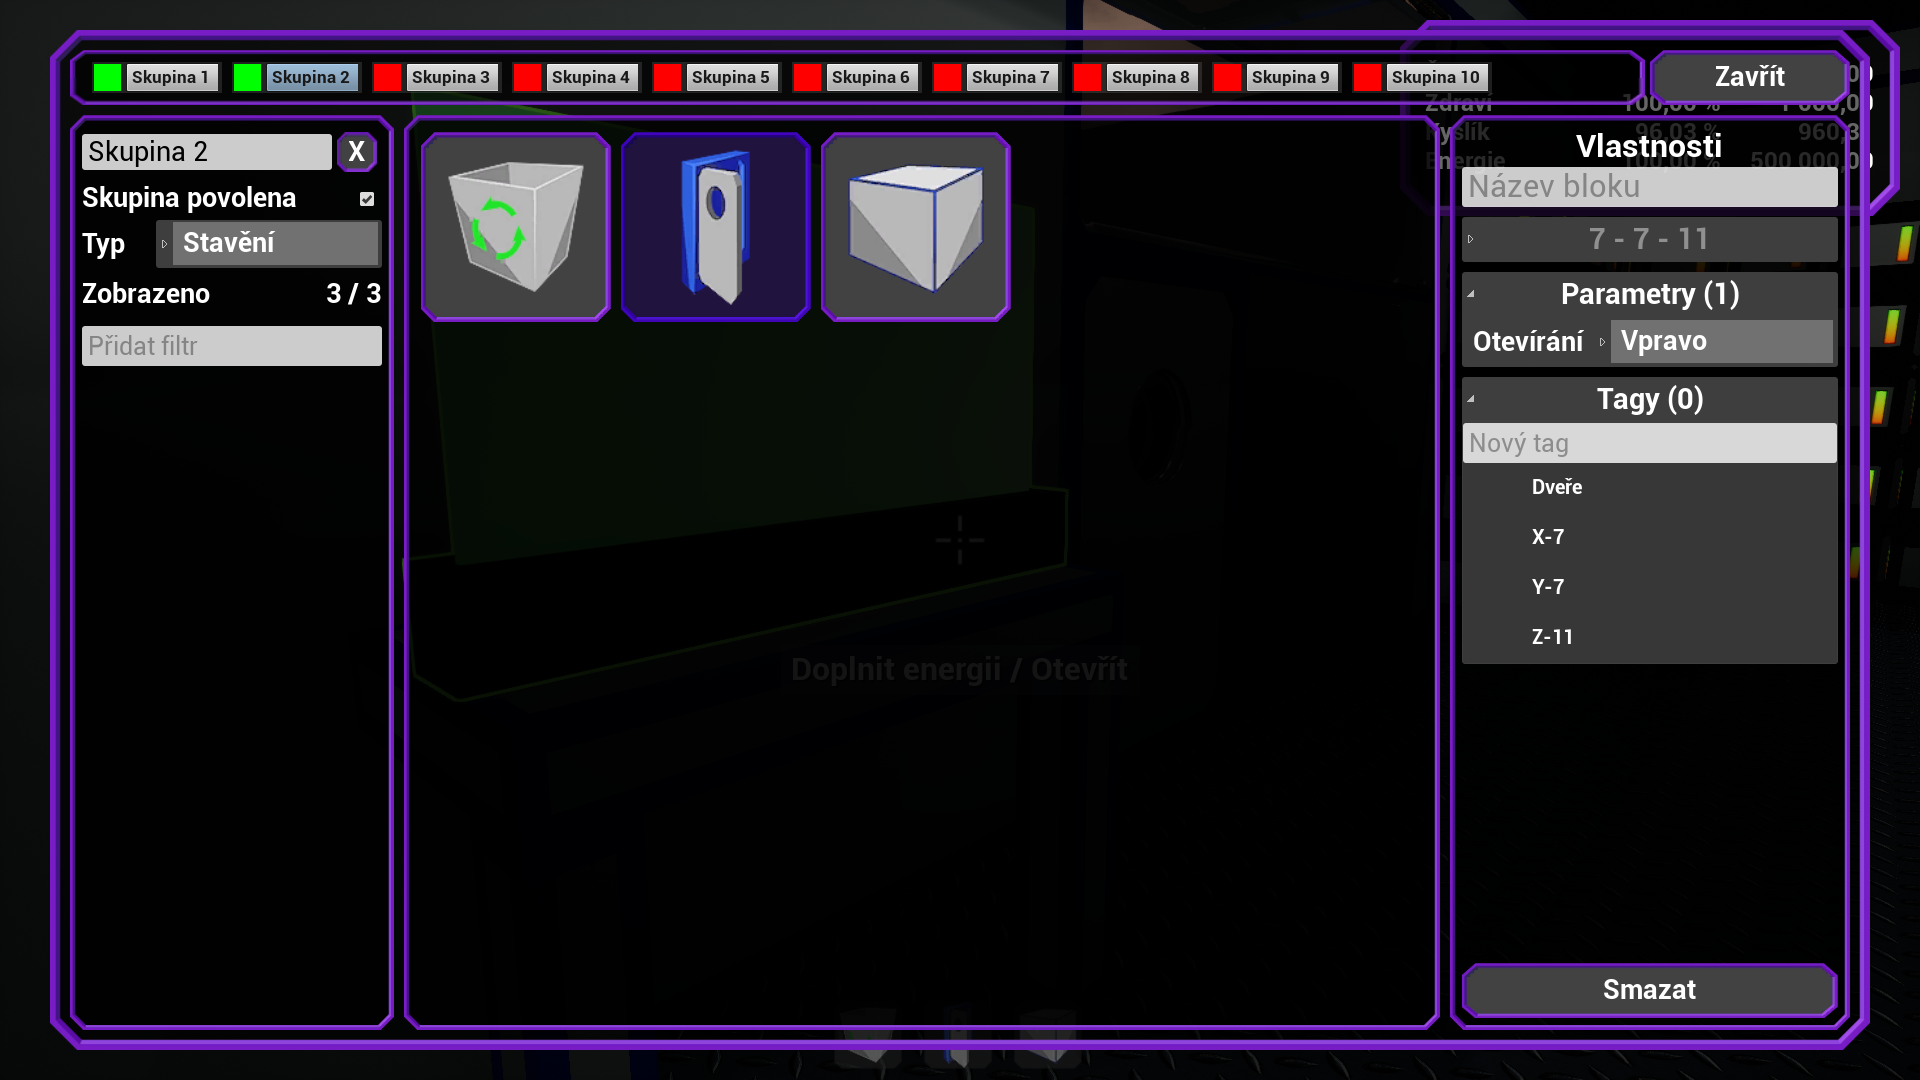
\includegraphics[ width=140mm]{../img/user/inventory/6itemWithParams}

\caption{Inventář - Nastavení}
\label{fig:user_inventory_6itemWithParams}

\end{figure}


\FloatBarrier
%!TEX root = ../prace.tex

\section{Terminál}

Pro informaci o aktuálním stavu sítě je nutné použít \textbf{Terminál}. Levým tlačítkem je možné rychle doplnit energii hráče, pravým pak otevřít ovládací obrazovku.

\begin{figure}[!h]\centering
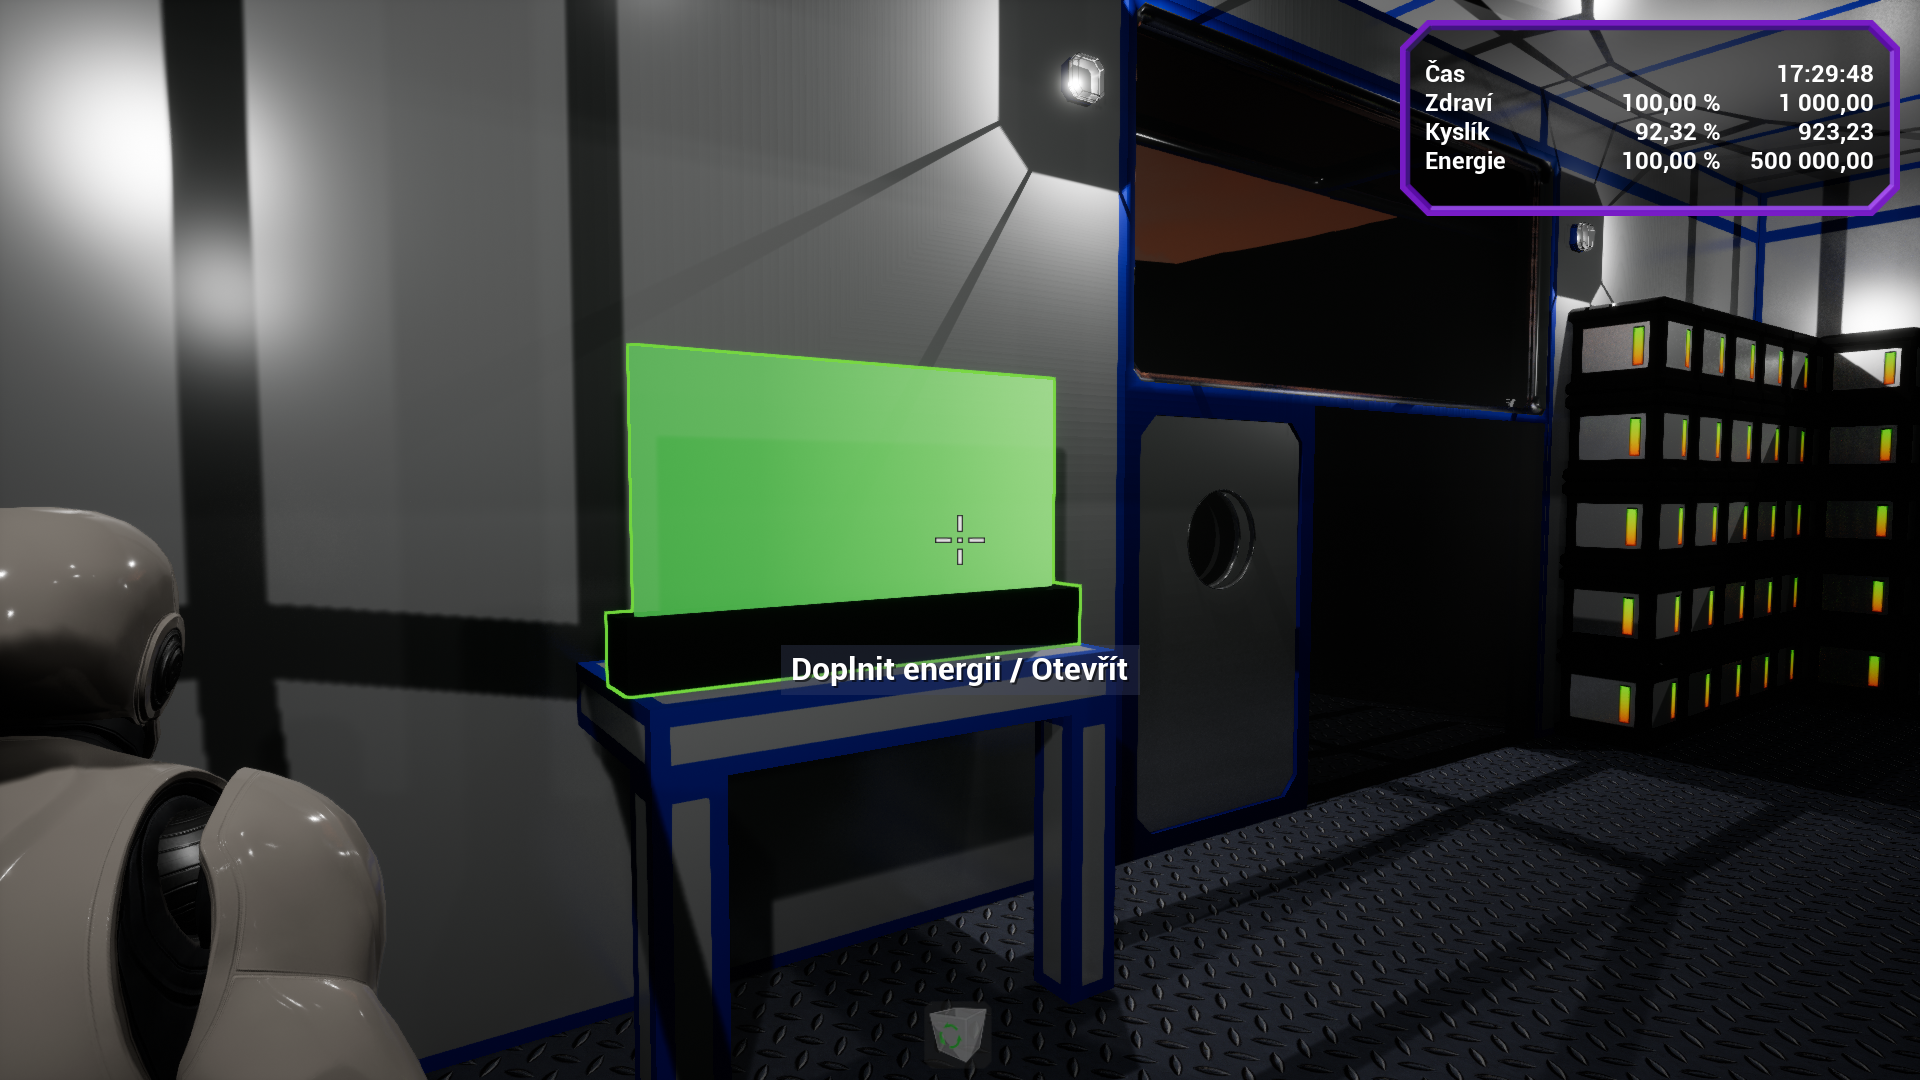
\includegraphics[ width=140mm]{../img/user/terminal/0terminalOverall}

\caption{Terminál - ve hře}
\label{fig:user_terminal_0terminalOverall}

\end{figure}

\FloatBarrier

V \textit{horní} části je vidět selektor obrazovky. Jeho rozkliknutím (více v obrázku \ref{fig:user_terminal_3terminalCtorSelector}) je možné zvolit výchozí obrazovku, nebo jeden z \textbf{Konstruktoru objektů}, které jsou v dispozici v síti.




\begin{figure}[!h]\centering
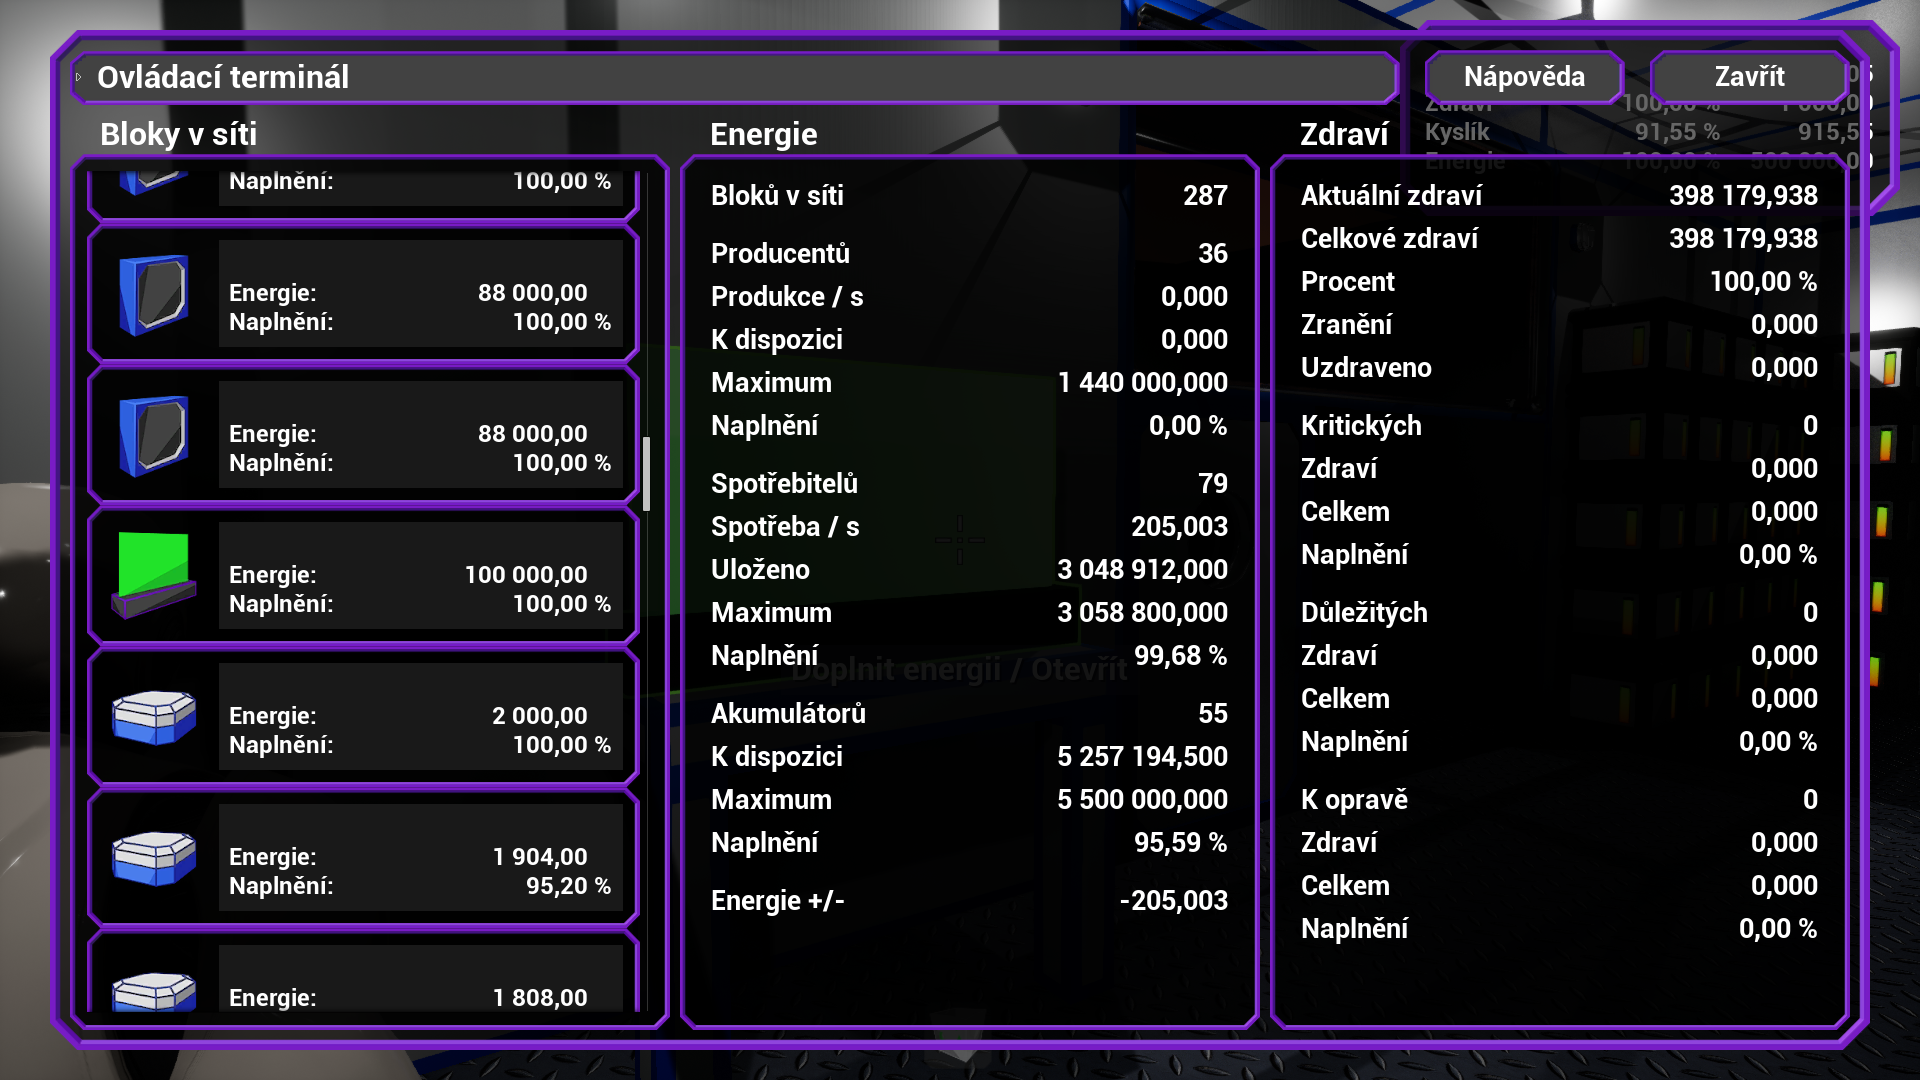
\includegraphics[ width=140mm]{../img/user/terminal/1terminalInfo}

\caption{Terminál - výchozí obrazovka}
\label{fig:user_terminal_1terminalInfo}

\end{figure}

\FloatBarrier
V \textit{levé} části je vidět seznam význačných bloků. \textit{Uprostřed} jsou vidět energetické informace o síti. \textit{Vpravo} je pak možné sledovat aktuální zdravotní stav sítě a bloků v síti.

Tlačítkem \textbf{Nápověda} je možné zobrazit informace o ovládání hry a přiřazených klávesách pro jednotlivé úkony.

\begin{figure}[!h]\centering
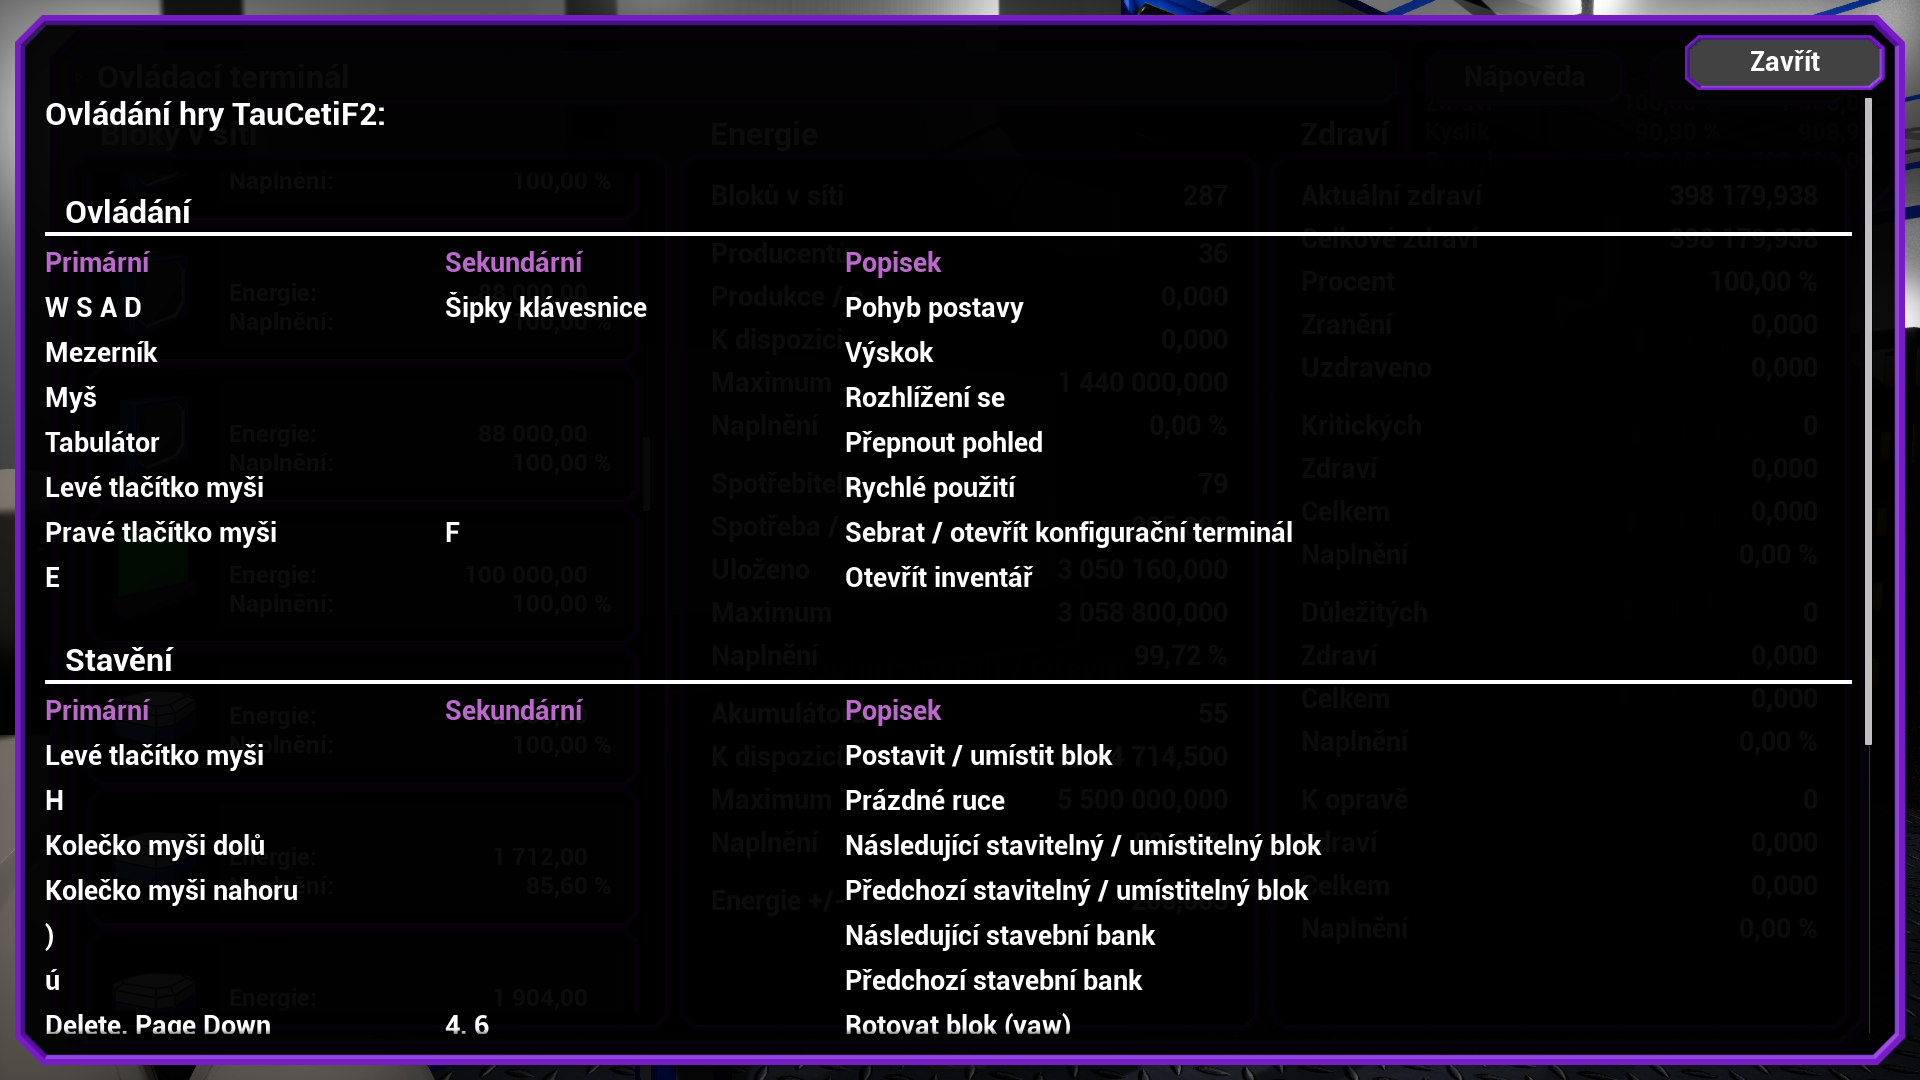
\includegraphics[ width=140mm]{../img/user/terminal/2terminalHelp}

\caption{Terminál - nápověda}
\label{fig:user_terminal_2terminalHelp}

\end{figure}

\FloatBarrier

Selektor dostupných obrazovek:

\begin{figure}[!h]\centering
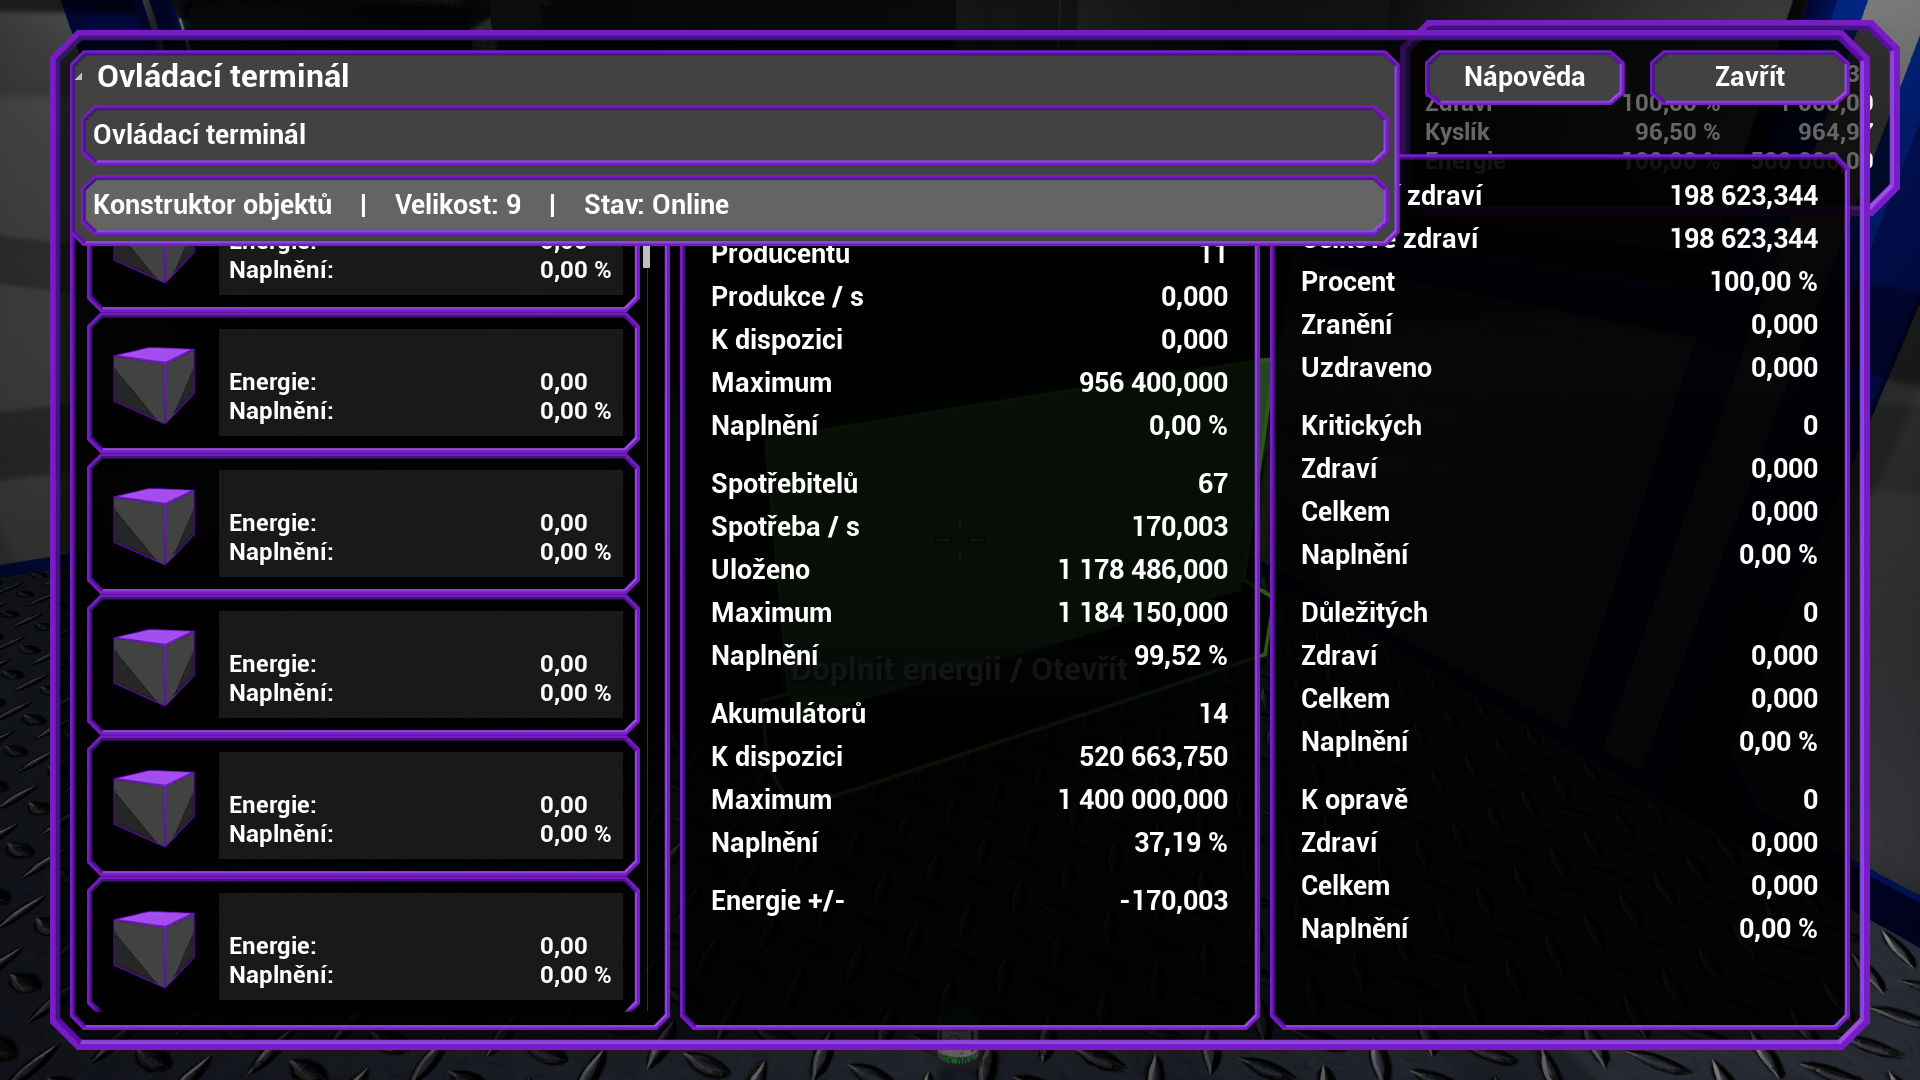
\includegraphics[ width=140mm]{../img/user/terminal/3terminalCtorSelector}

\caption{Terminál - selektor obrazovek}
\label{fig:user_terminal_3terminalCtorSelector}

\end{figure}

\FloatBarrier

Pokud vybereme \textbf{Konstruktor objektů}, vidíme seznam dostupných bloků, které můžeme zkonstruovat. Pokud to pro některé nelze (třeba z důvodu omezení velikosti - konstruktor je na daný objekt příliš malý), blok není aktivní a nelze ho zvolit.


\begin{figure}[!h]\centering
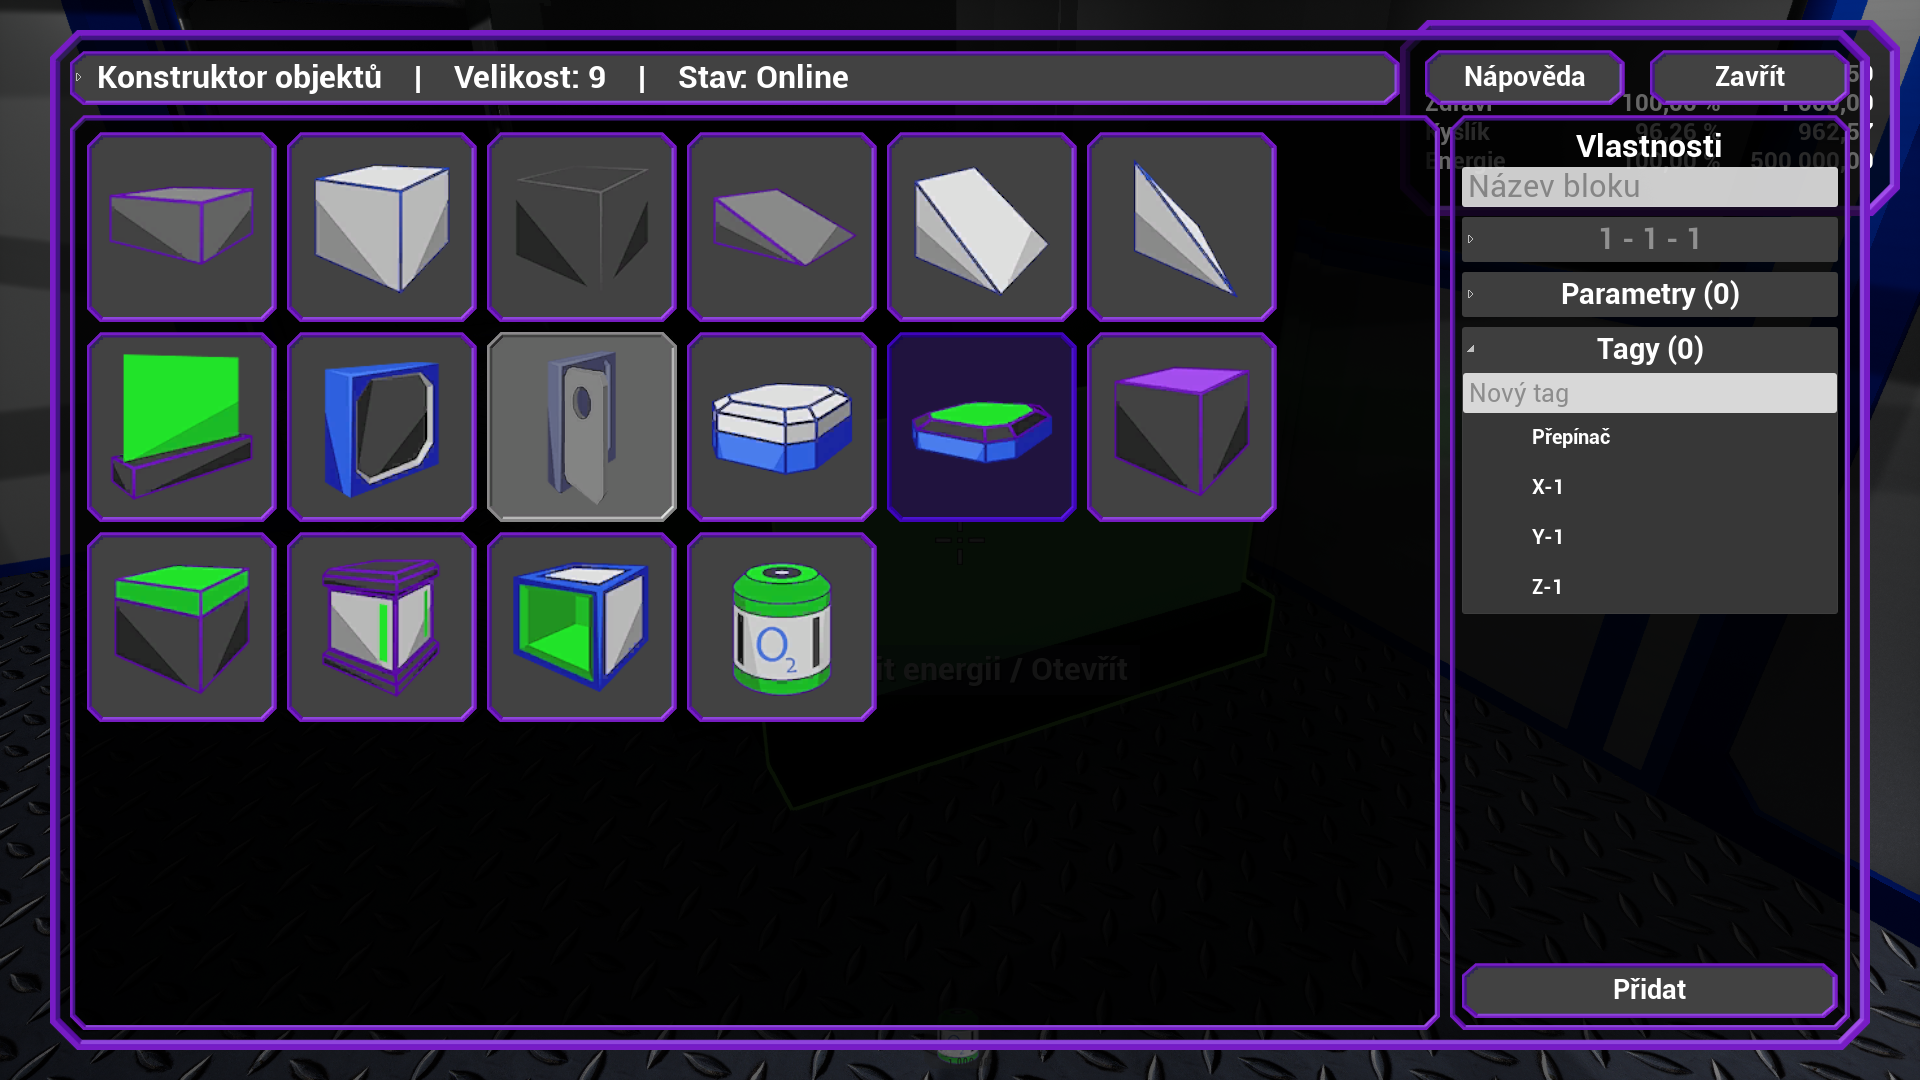
\includegraphics[ width=140mm]{../img/user/terminal/4builderSmall}

\caption{Terminál - konstruktor objektů}
\label{fig:user_terminal_4builderSmall}

\end{figure}

\FloatBarrier

V sekci \textit{Nastavení} je možné kromě tagů definovat i požadovanou velikost a to až do velikosti konstruktoru, nebo globálního omezení 20 násobku  základní kostky.

\begin{figure}[!h]\centering
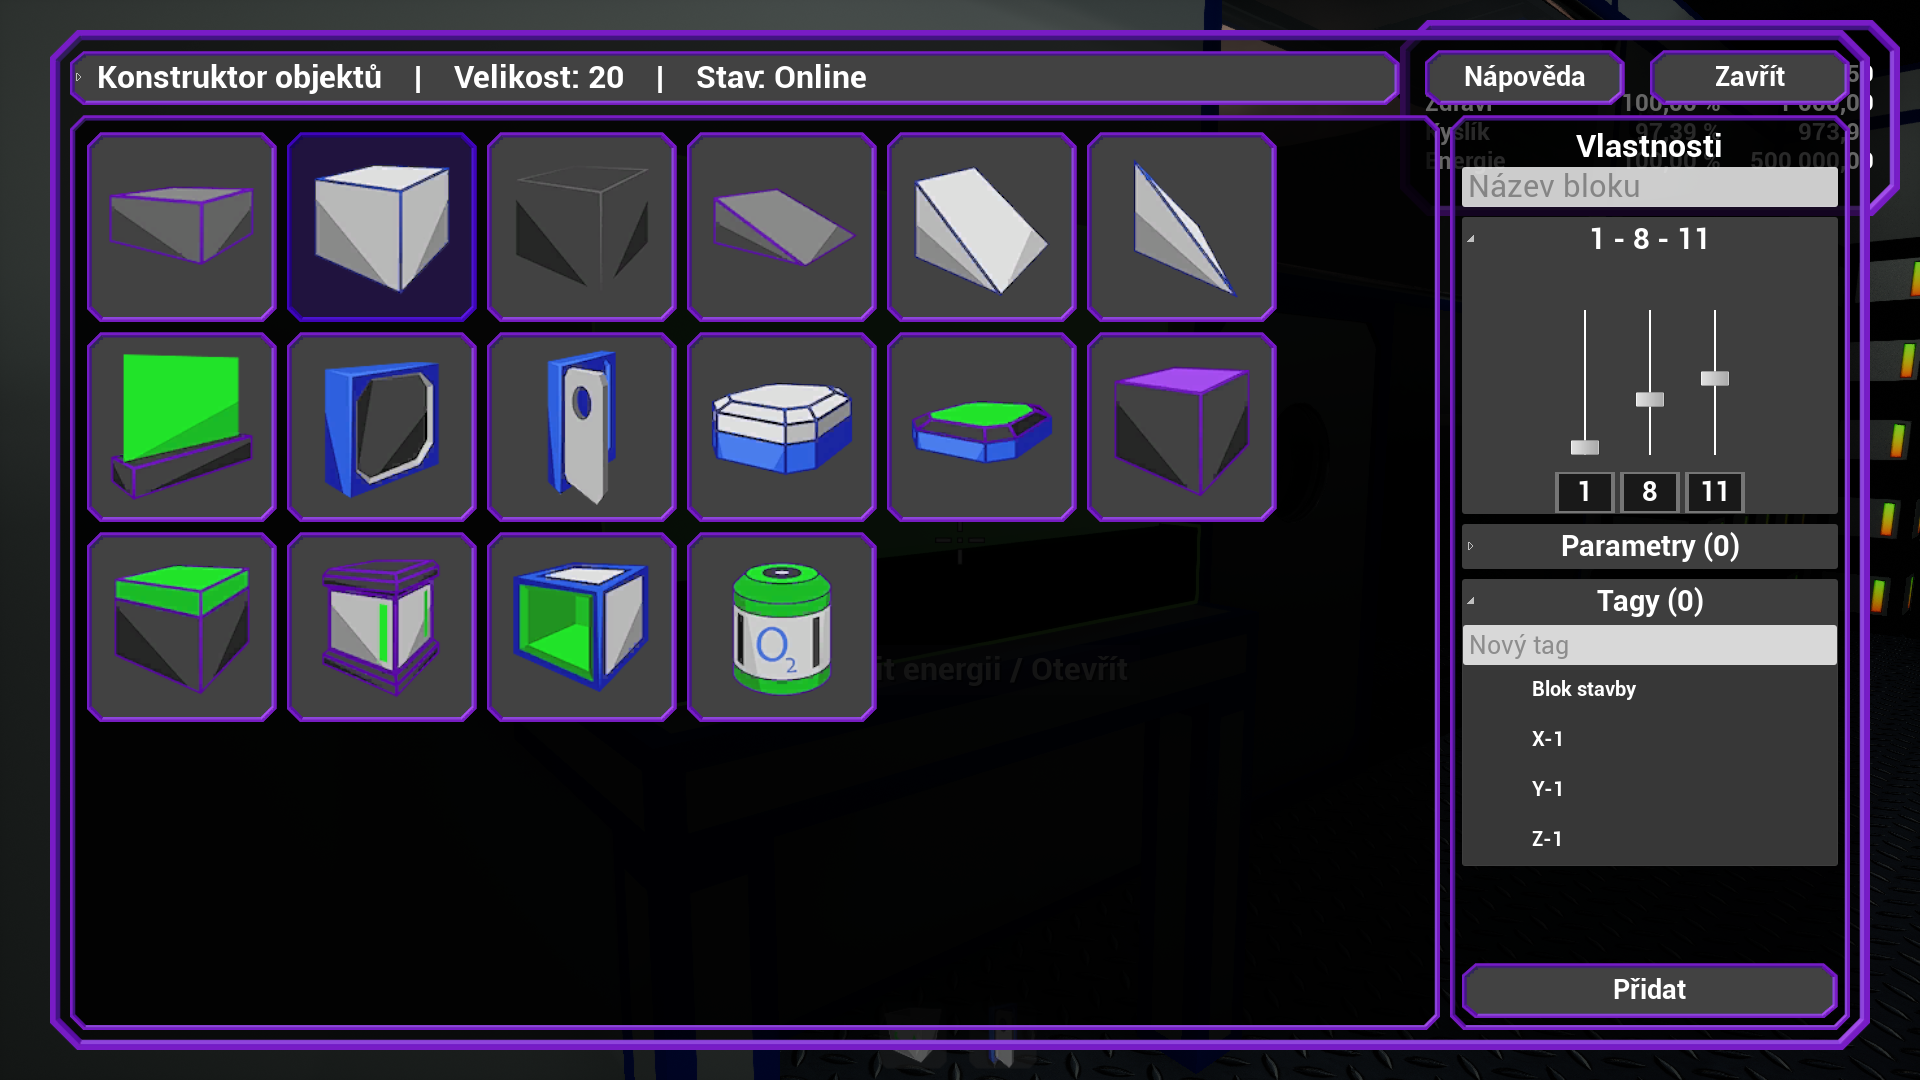
\includegraphics[ width=140mm]{../img/user/terminal/5builderSize}

\caption{Terminál - Nastavení velikosti}
\label{fig:user_terminal_5builderSize}

\end{figure}

\FloatBarrier

Některé bloky, třeba \textbf{Dveře} požadují dodatečné parametry, které ovlivňují jejich výsledné chování. V našem případě to je smysl otevírání dveří při čelním pohledu. Na obrázku je vidět stav po rozkliknutí.

\begin{figure}[!h]\centering
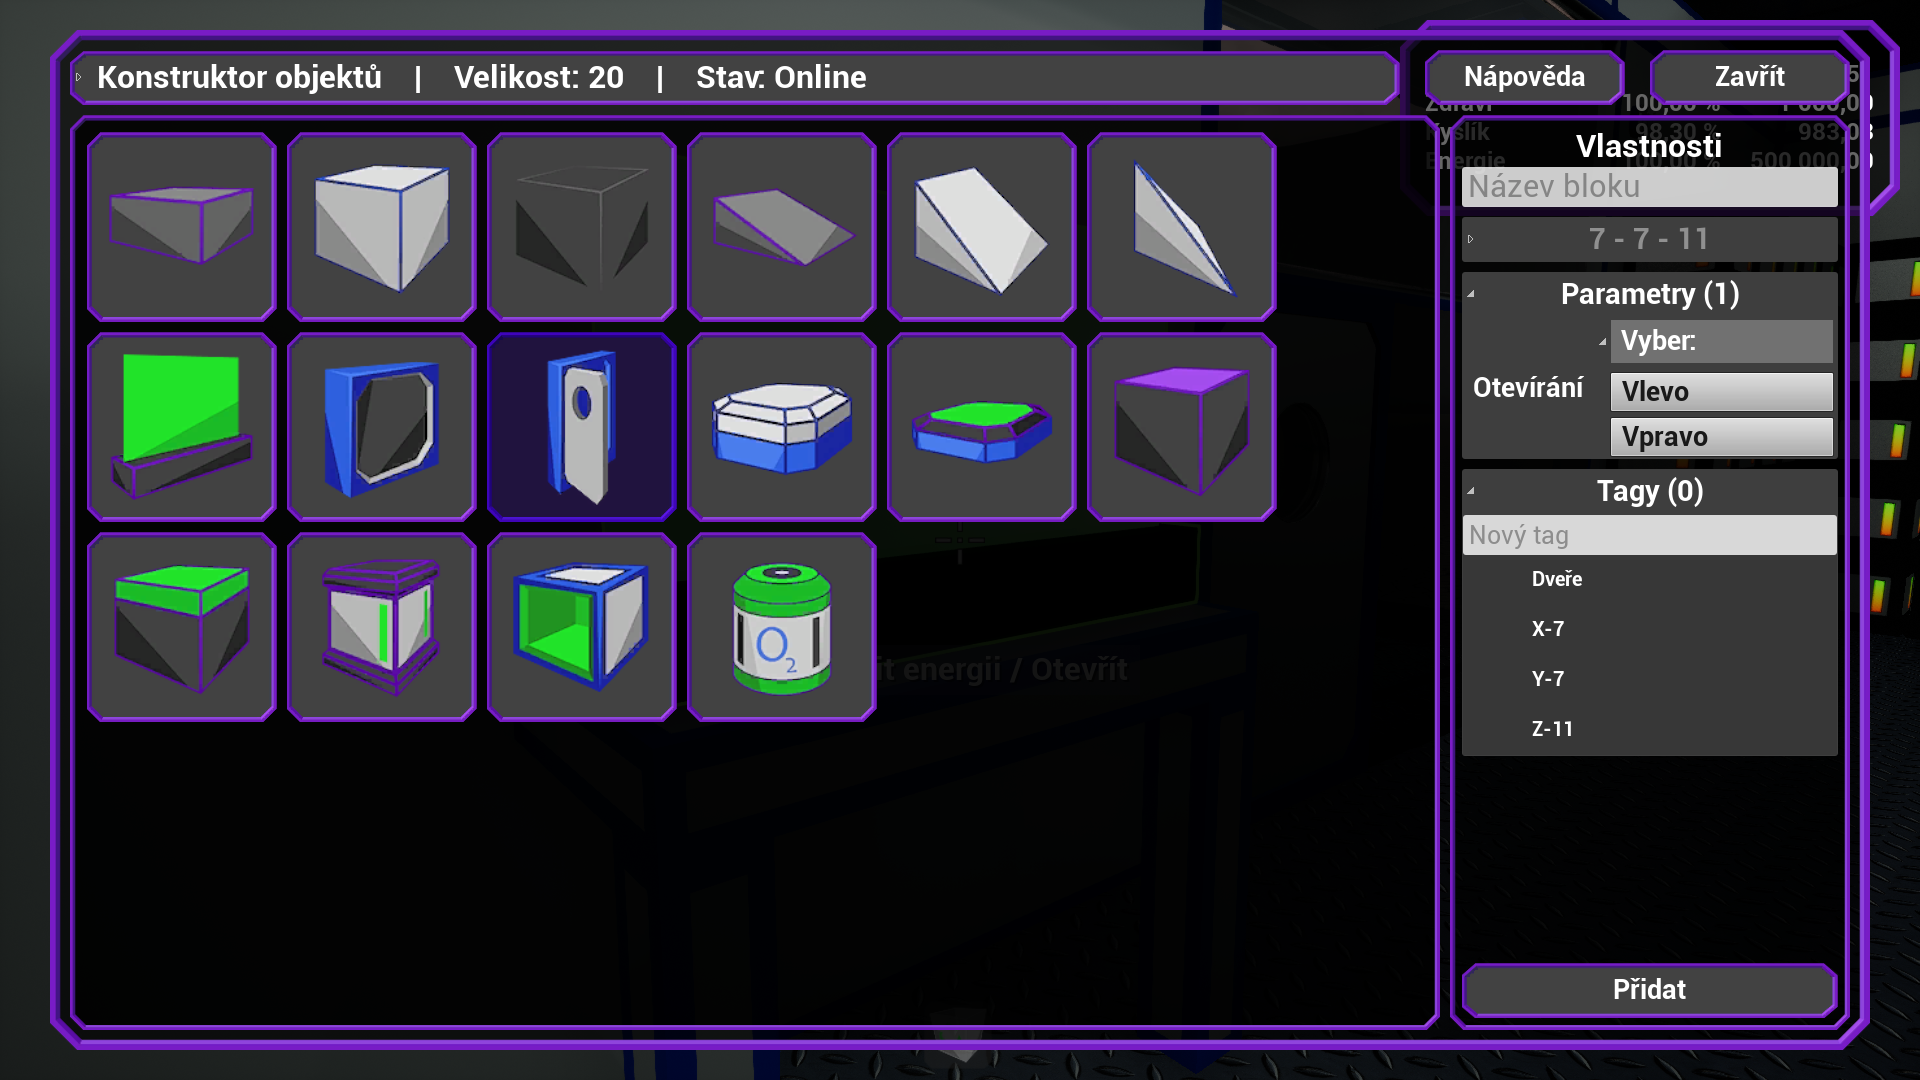
\includegraphics[ width=140mm]{../img/user/terminal/6builderParams}

\caption{Terminál - Nastavení parametrů}
\label{fig:user_terminal_6builderParams}

\end{figure}

\FloatBarrier
%!TEX root = ../../prace.tex

\section{Stavební akce}

\textbf{Destruktor} umožňuje mazat bloky. Po jeho výběru je vidět červený outline vybraného bloku.

\begin{figure}[!ht]\centering
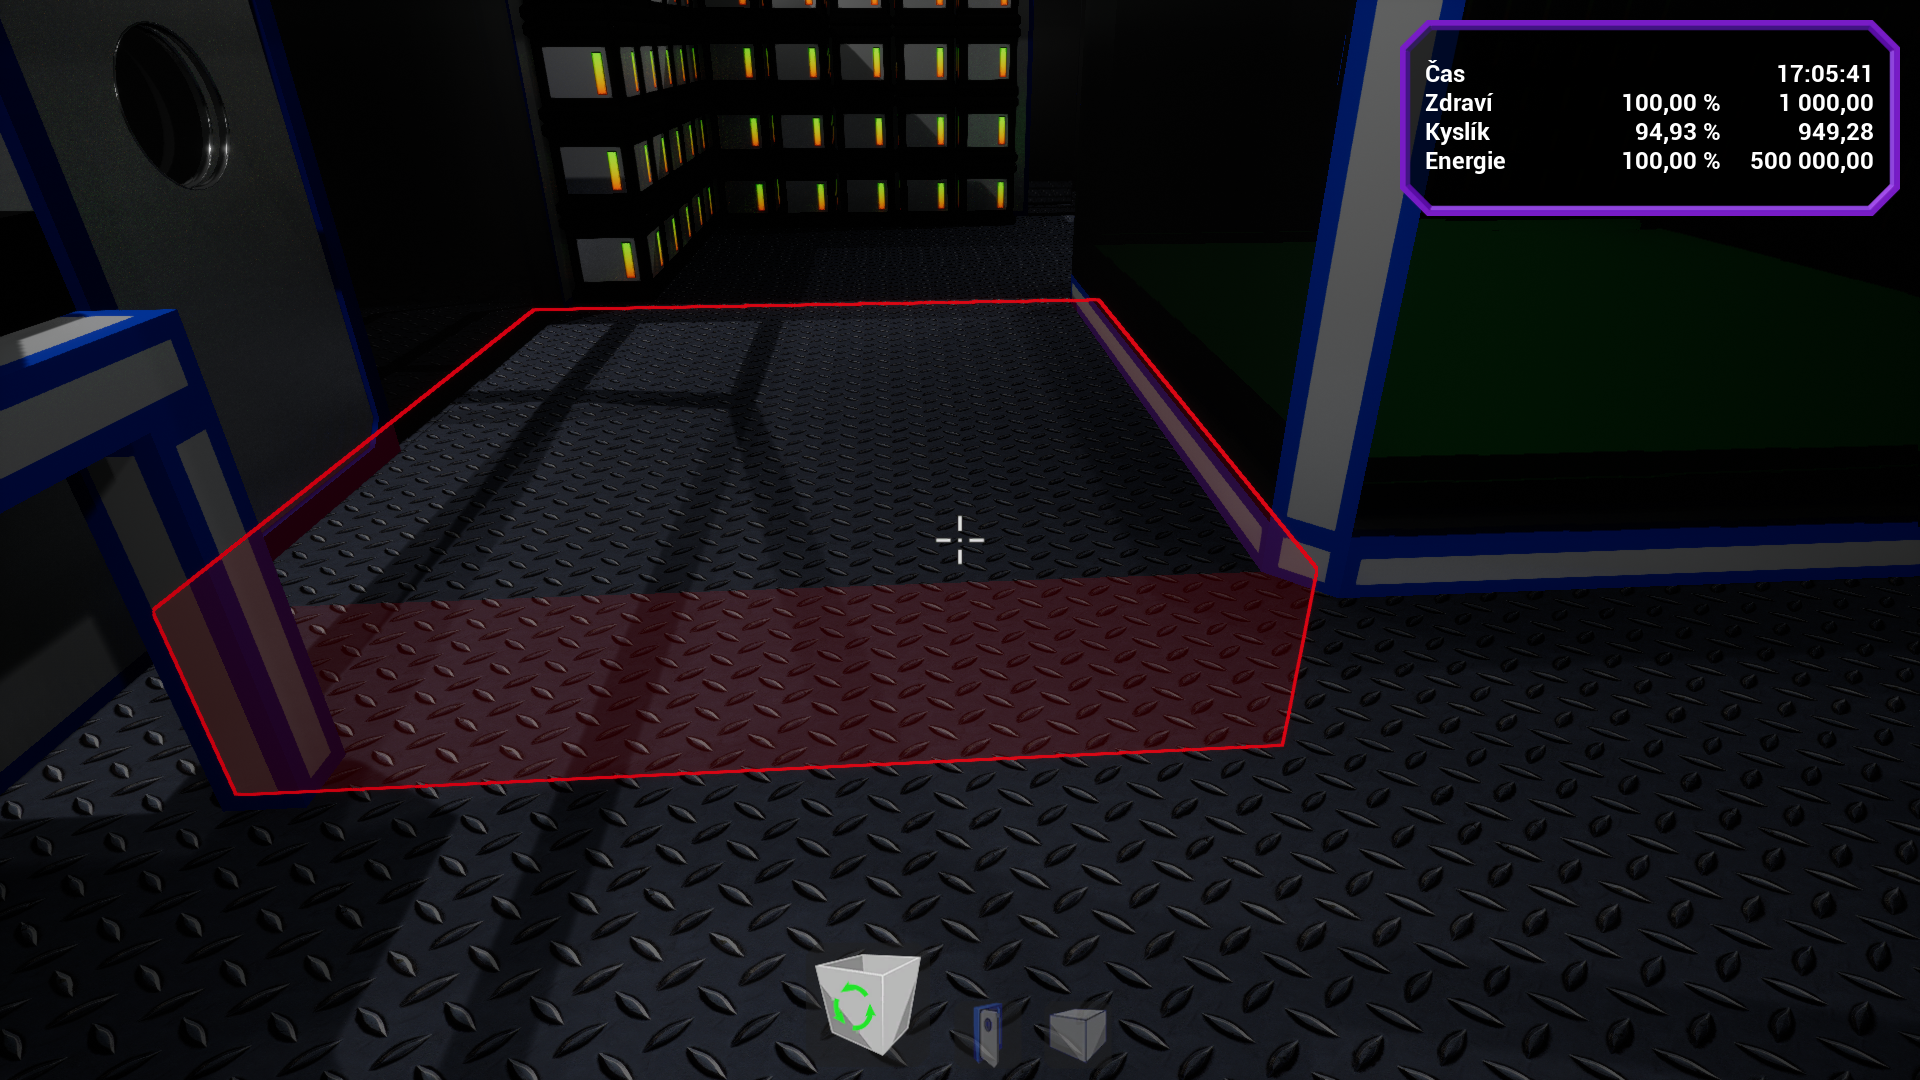
\includegraphics[ width=140mm]{../img/user/buildActions/delete}

\caption{Stavění -- smazat}
\label{fig:user_buildActions_delete}

\end{figure}

\FloatBarrier

Pokud vybereme umístění nového bloku, vidíme žlutě hranice sousedního bloku, ke kterému blok přistavujeme. Stavěný / umisťovaný blok musí mít dostatečné místo pro svoje umístění. Dále je potřeba mít s~sebou dostatečně velkou zásobu energie (dle energetické náročnosti bloku).

\begin{figure}[!ht]\centering
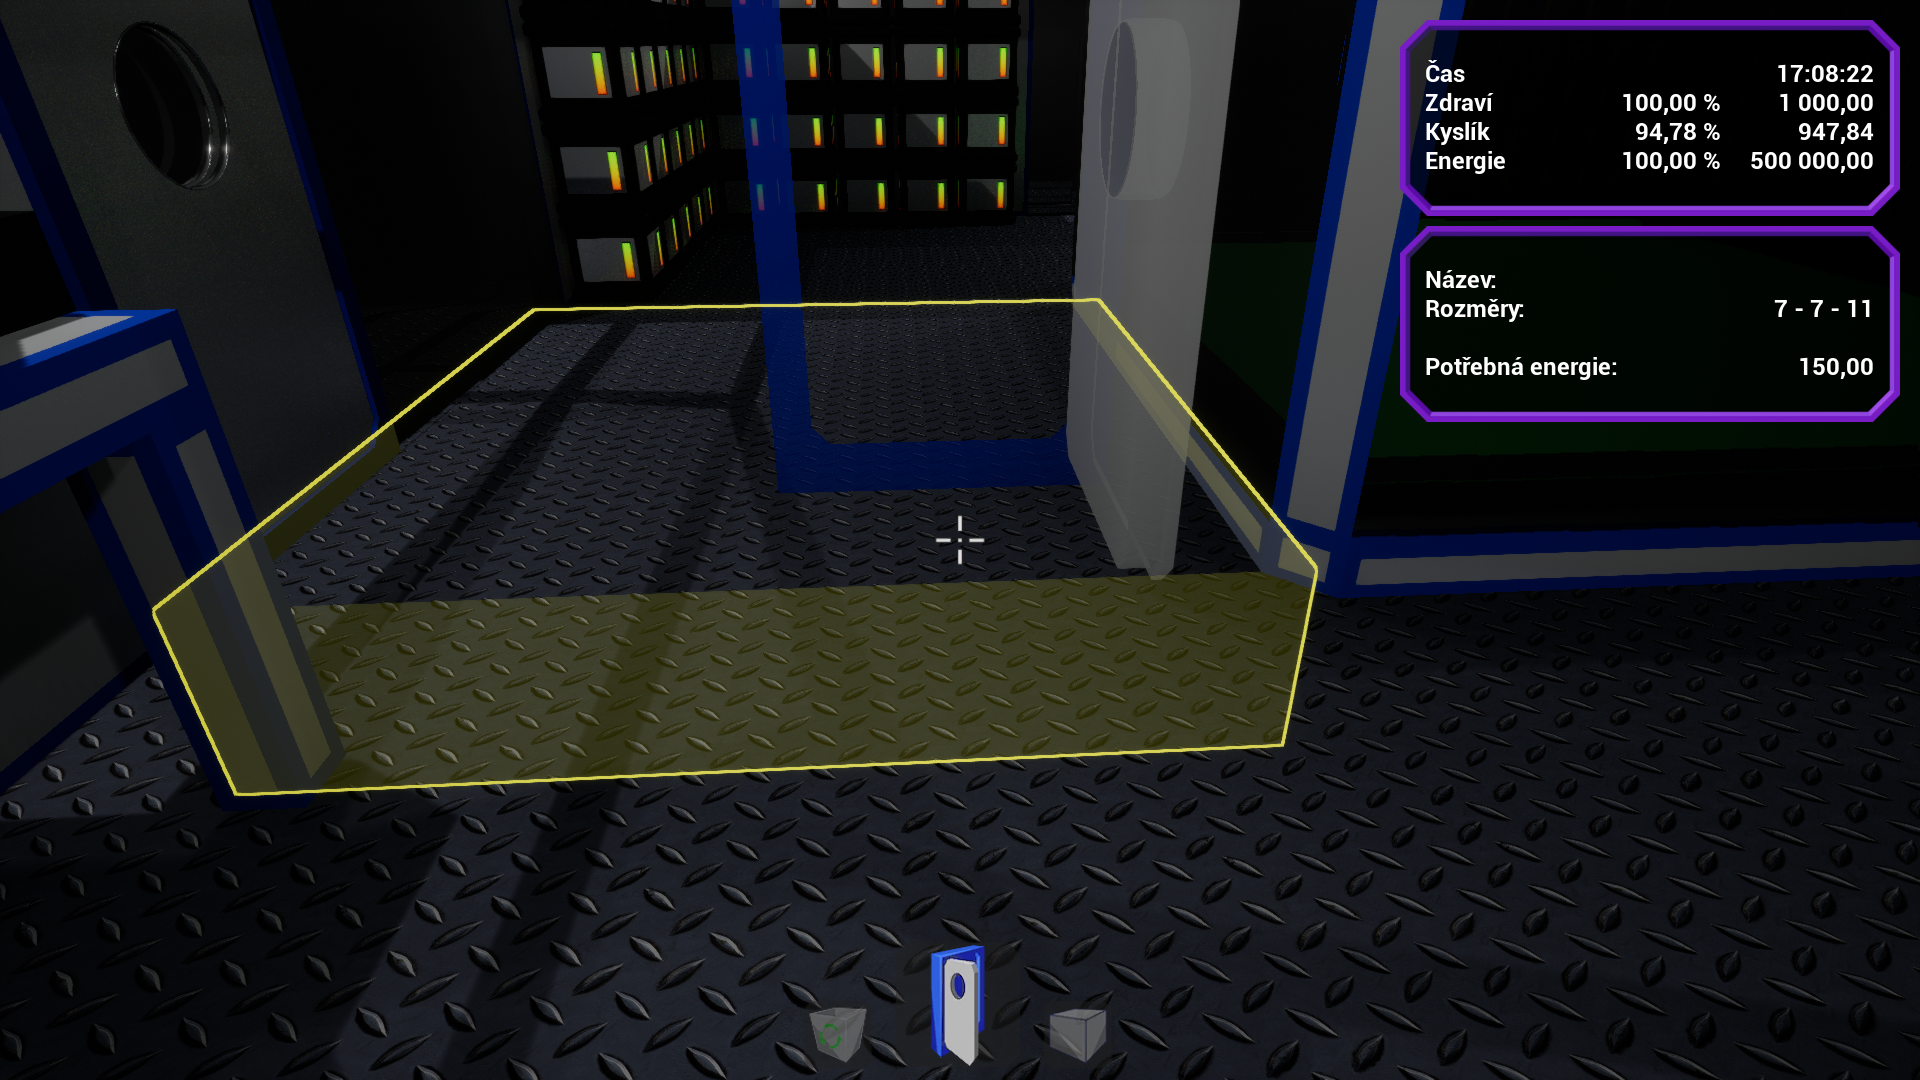
\includegraphics[ width=140mm]{../img/user/buildActions/place}

\caption{Stavění -- umístit}
\label{fig:user_buildActions_place}

\end{figure}

\FloatBarrier

Blok je též možný rotovat (Klávesy v~sekci Insert .. Page Down, případně jejich ekvivalenty 7,8,9,4,5,6).

\begin{figure}[!ht]\centering
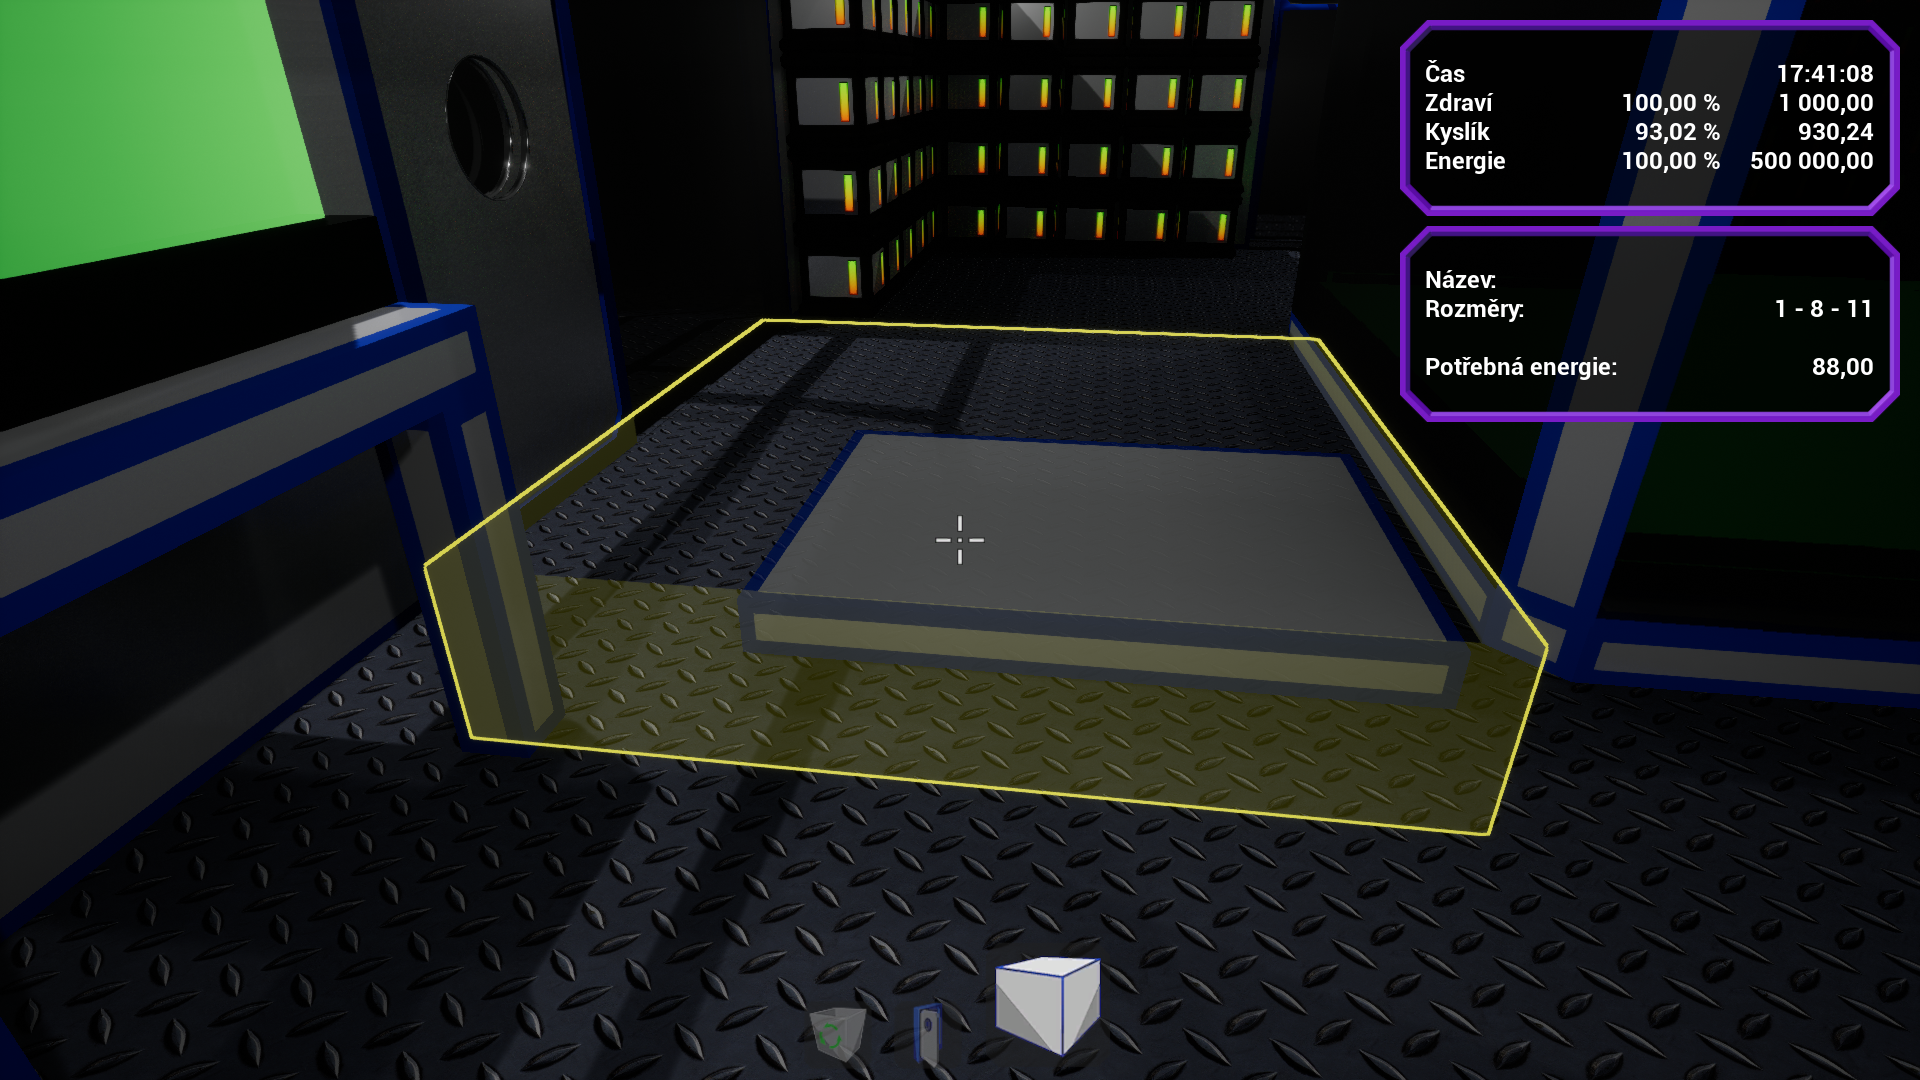
\includegraphics[ width=140mm]{../img/user/buildActions/place_Rotate}

\caption{Stavění -- rotace}
\label{fig:user_buildActions_place_Rotate}

\end{figure}

\FloatBarrier

Pokud bylo umístění v~pořádku, blok již není nadále průhledný a~hráči ubyla energie. Pokud je zapnut kreativní mód, energie samozřejmě neubývá.

\begin{figure}[!ht]\centering
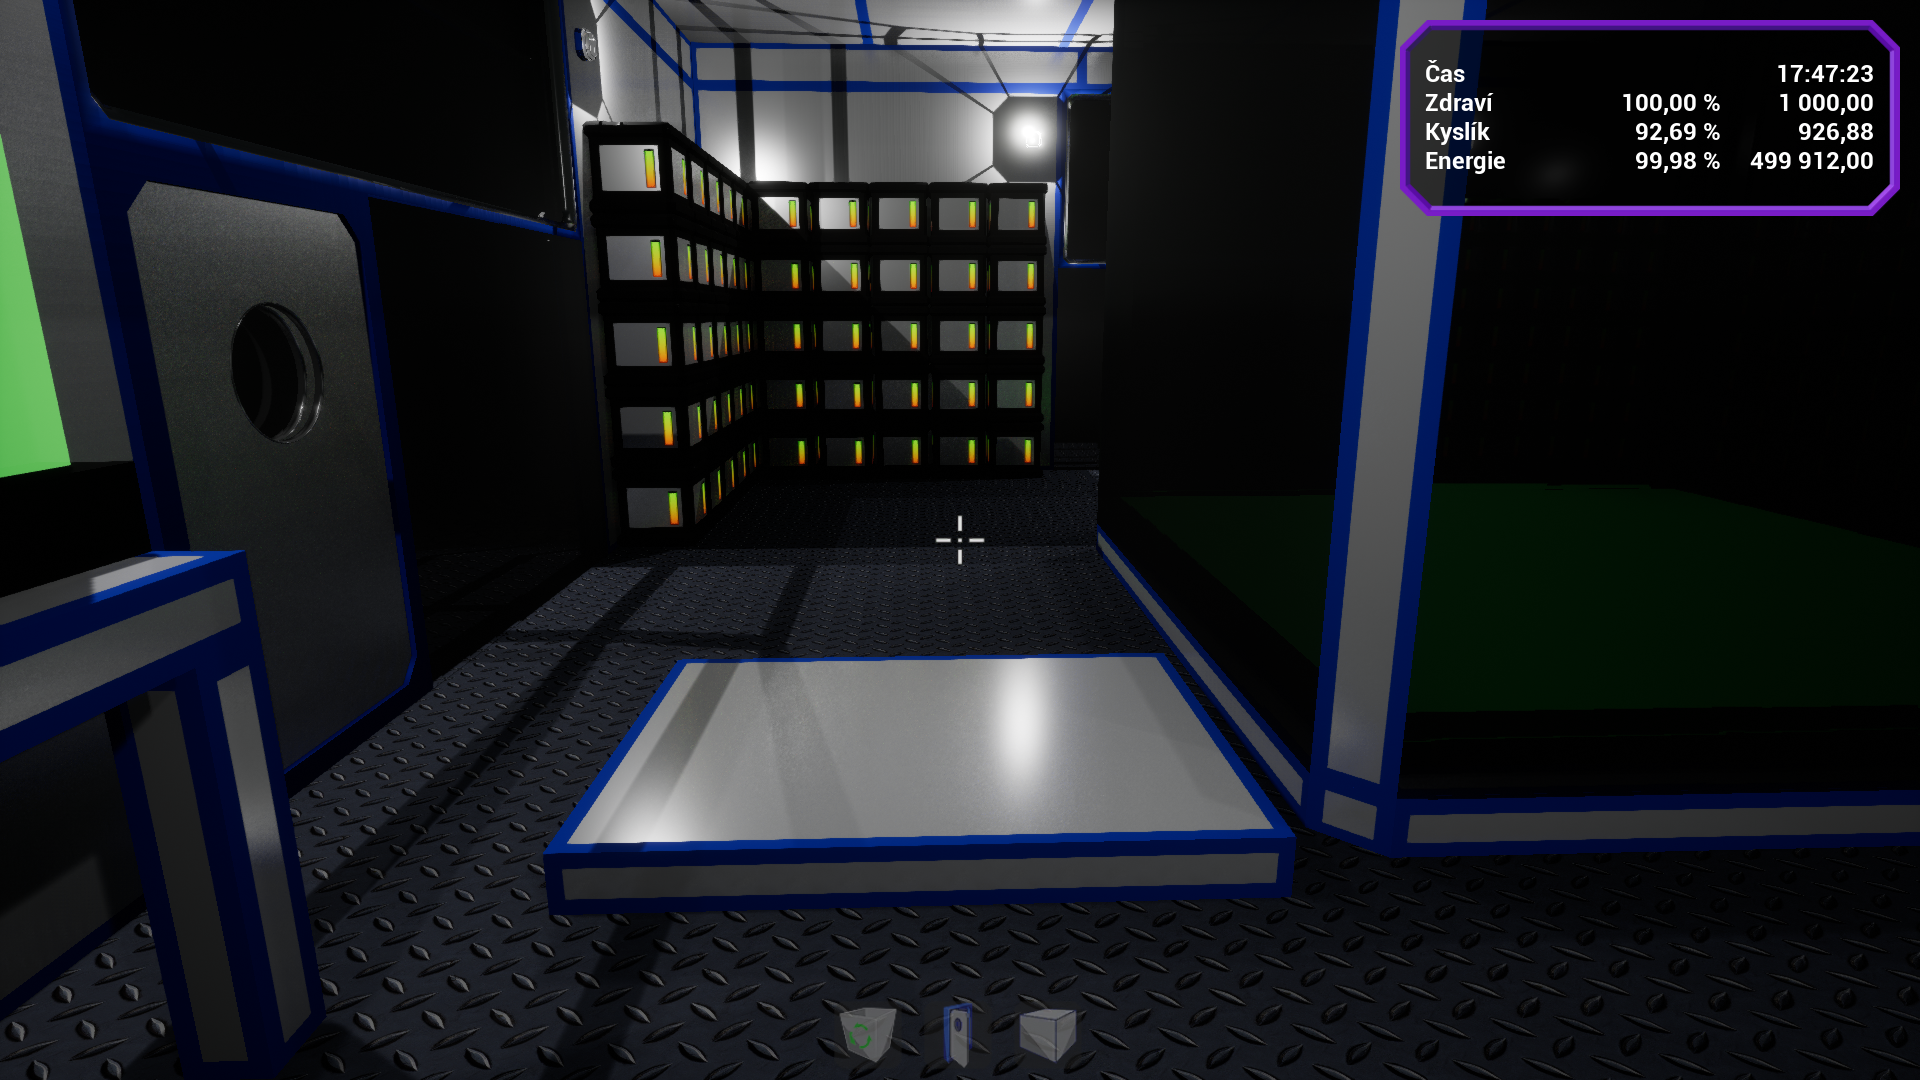
\includegraphics[ width=140mm]{../img/user/buildActions/placeAfter}

\caption{Stavění -- po umístění}
\label{fig:user_buildActions_placeAfter}

\end{figure}


\FloatBarrier
%!TEX root = ../../prace.tex

\section{Umístitelné předměty}

Blok \textbf{Kyslíková bomba} je možné umístit do světa a pak si ho opět vzít do inventáře. Díky tomu je možné tyto bloky dále používat třeba pro plnění v \textbf{Plničce kyslíkových bomb}.
Blok je možné buď rovnou použít (levé tlačítko myši).
Tento blok zároveň rovnou ukazuje, kolik objemu je využito.

\begin{figure}[!ht]\centering
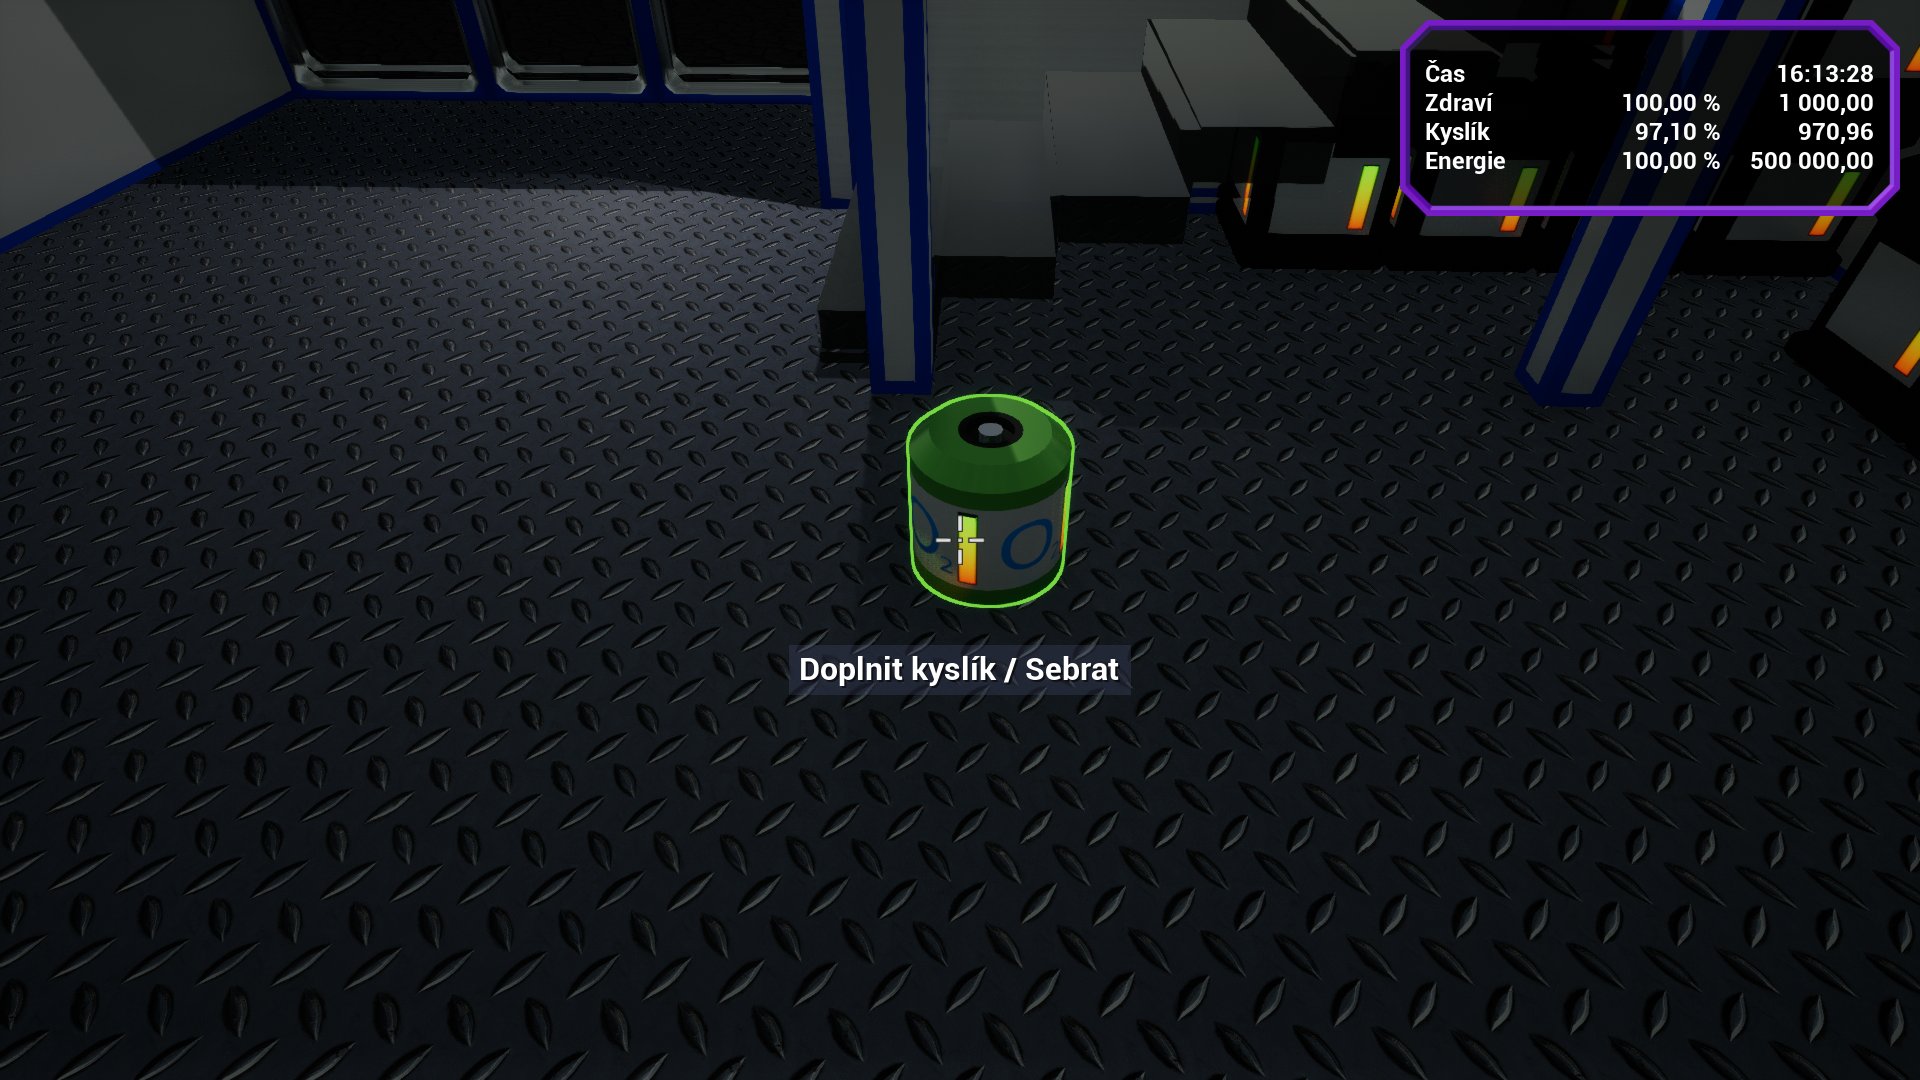
\includegraphics[ width=140mm]{../../img/user/tank/0tankFull}

\caption{Umístitelné předměty - plná kyslíková bomba}
\label{fig:user_tank_0tankFull}

\end{figure}

\FloatBarrier

Na dalším obrázku vidíme již částečně použitou kyslíkovou bombu. Pokud ji pravým tlačítkem myši sebereme a otevřeme si inventář a správnou skupinu (\textbf{Typ: Inventář} v nastavení skupiny), uvidíme tento blok v seznamu.

Požité tagy se při přidání do světa a opětovném sebrání zachovávají.

\begin{figure}[!ht]\centering
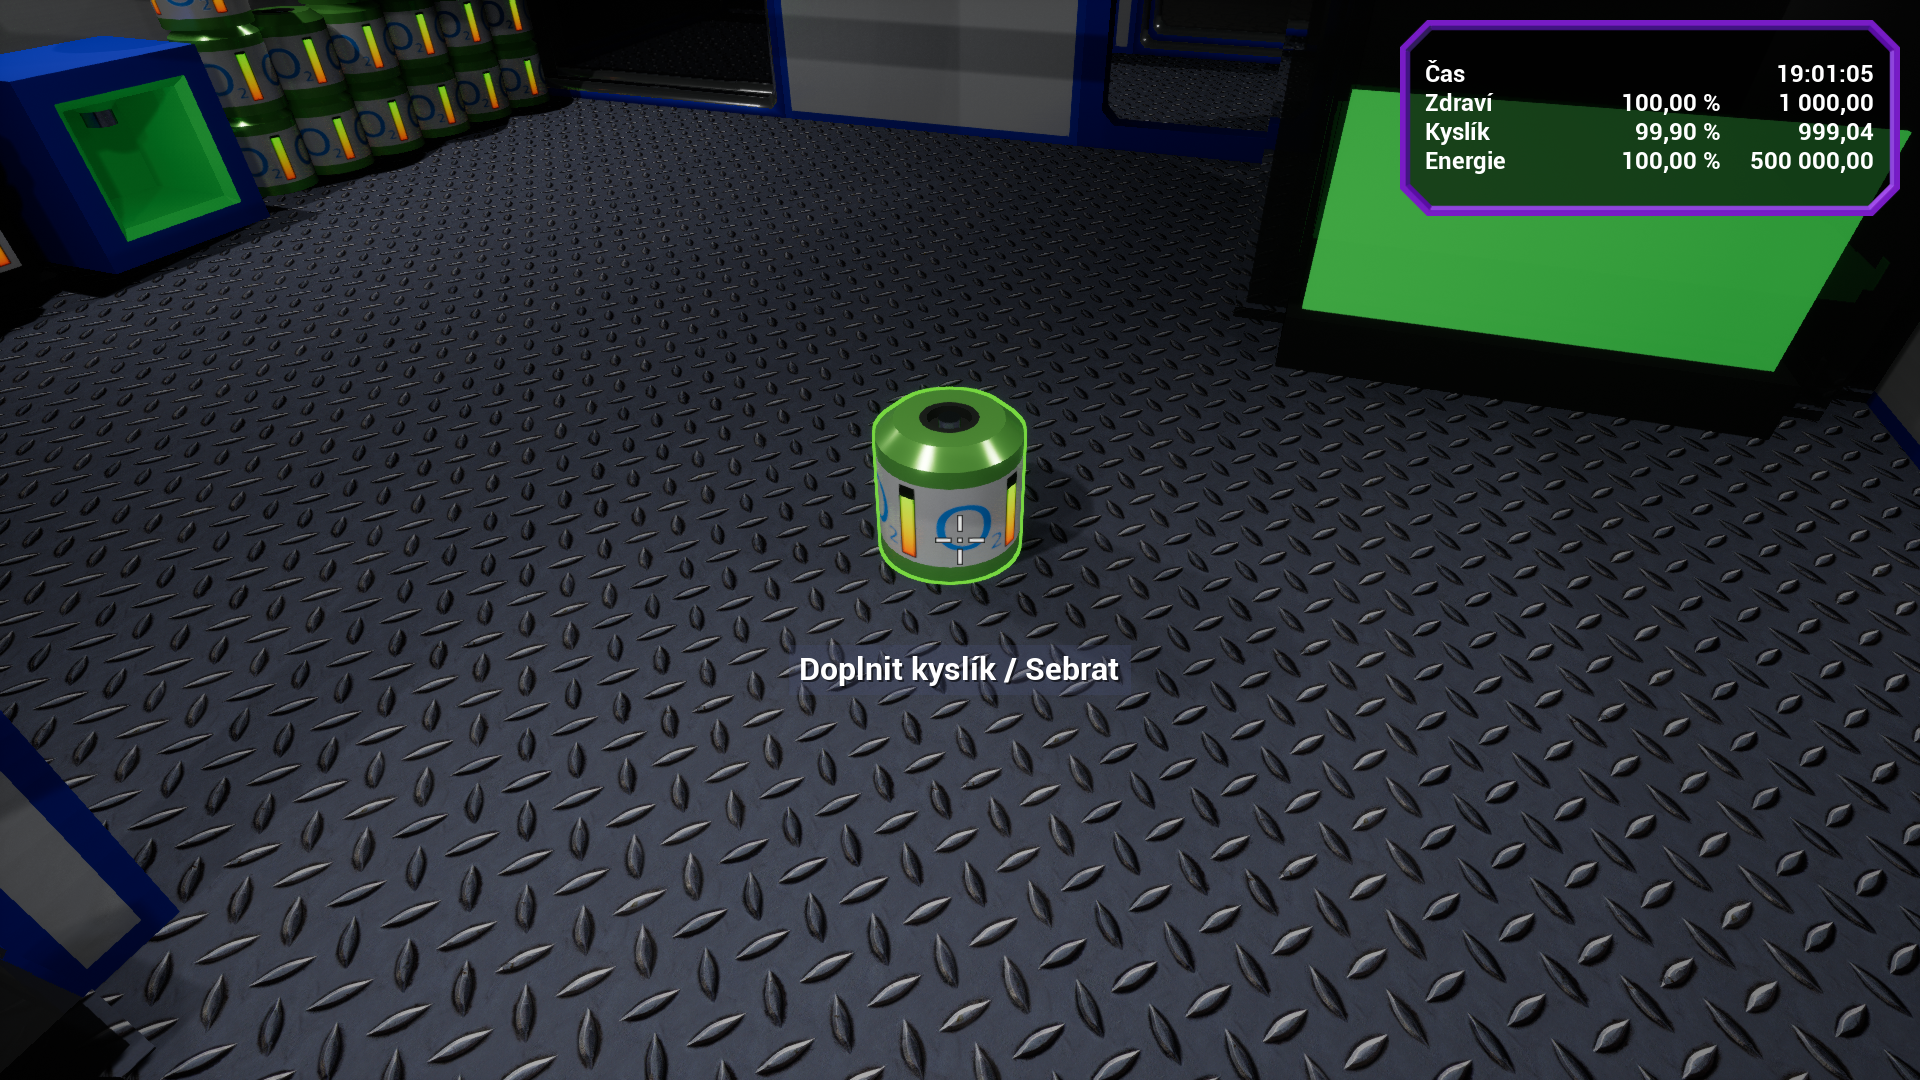
\includegraphics[ width=140mm]{../../img/user/tank/1tankAfterUse}

\caption{Umístitelné předměty - použitá bomba}
\label{fig:user_tank_1tankAfterUse}

\end{figure}

\FloatBarrier

Zároveň v inventáři můžeme vidět přesnou hodnotu naplnění bloku.

\begin{figure}[!ht]\centering
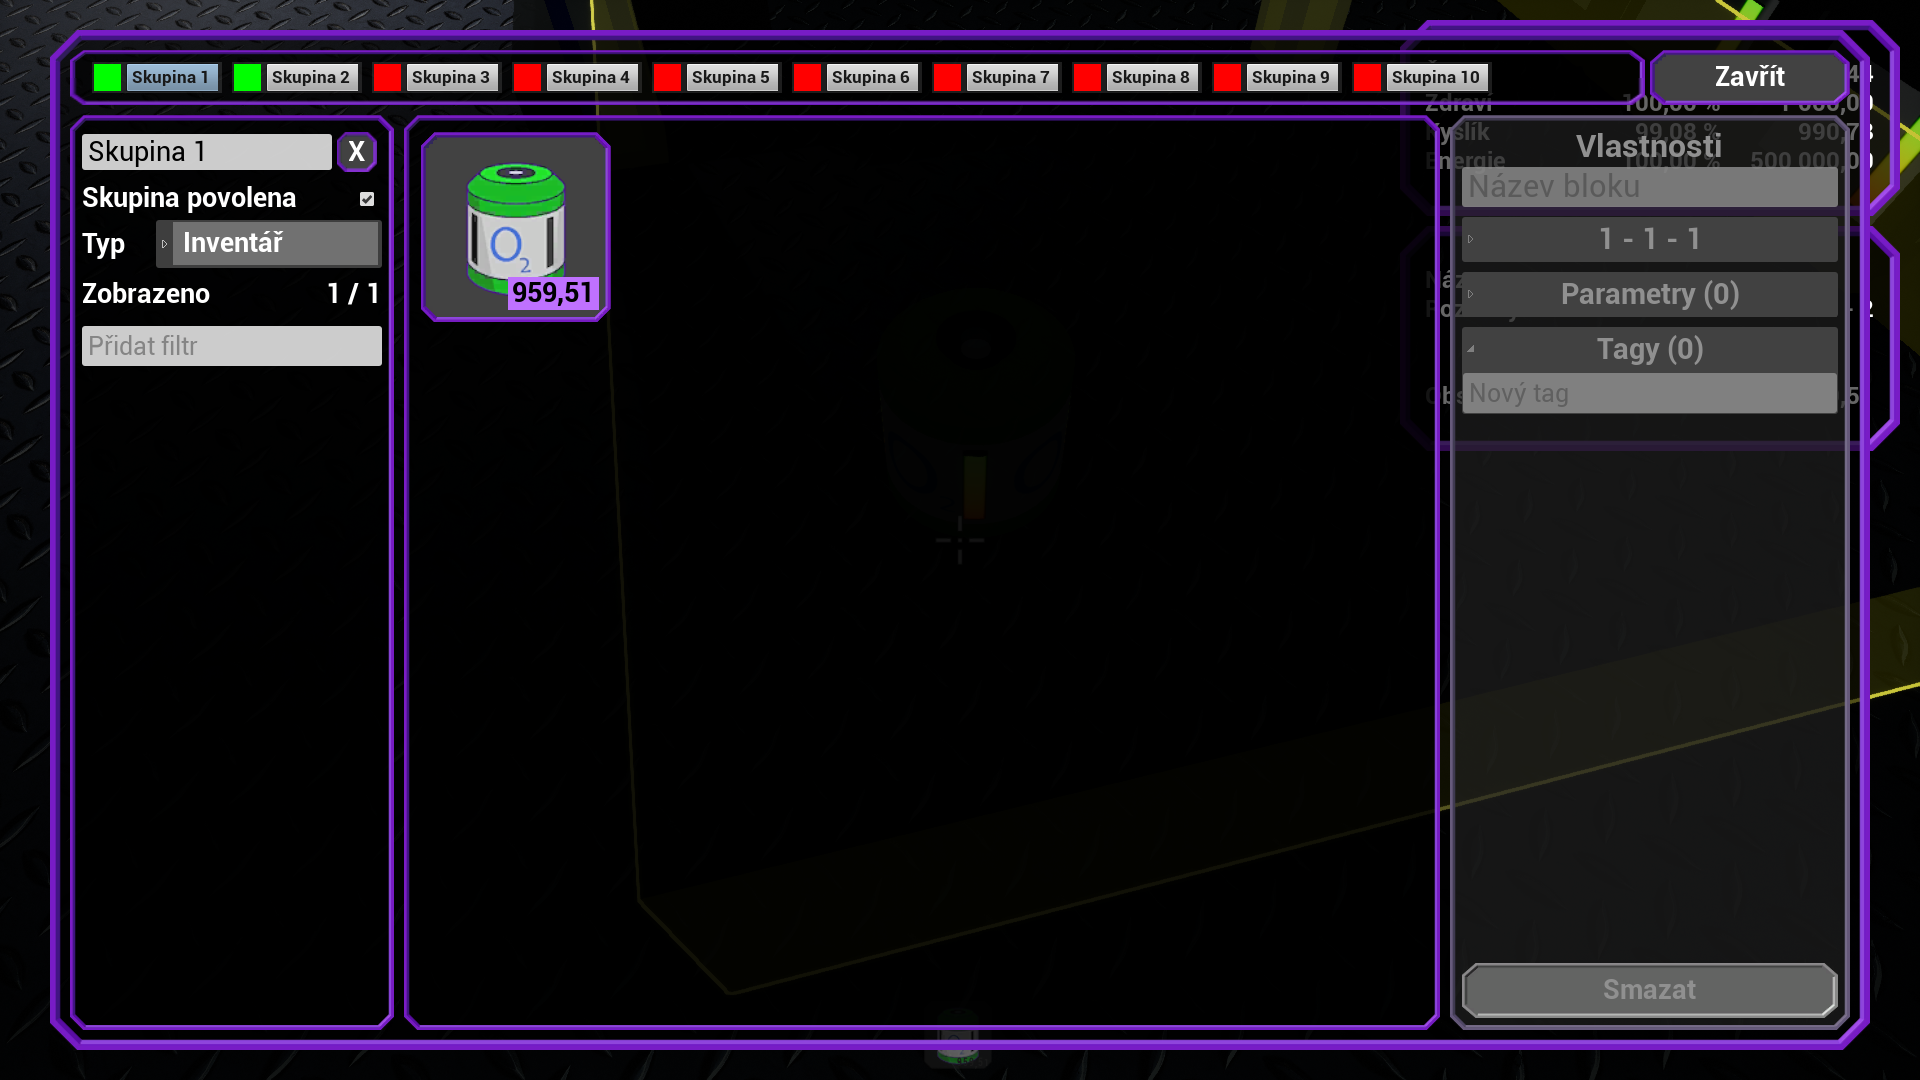
\includegraphics[ width=140mm]{../../img/user/tank/2tankInventory}

\caption{Umístitelné předměty - inventář}
\label{fig:user_tank_2tankInventory}

\end{figure}



\FloatBarrier
%!TEX root = ../../prace.tex

\section{Plnička kyslíkových bomb}

Kyslíkové bomby je potřeba opětovně naplnit, pokud byl jejich obsah spotřebován. Stejně jako u~Kyslíkové bomby, levým tlačítkem myši je možné rovnou doplnit zásoby kyslíku hráče. Pravým se pak otevře ovládací obrazovka.

\begin{figure}[!ht]\centering
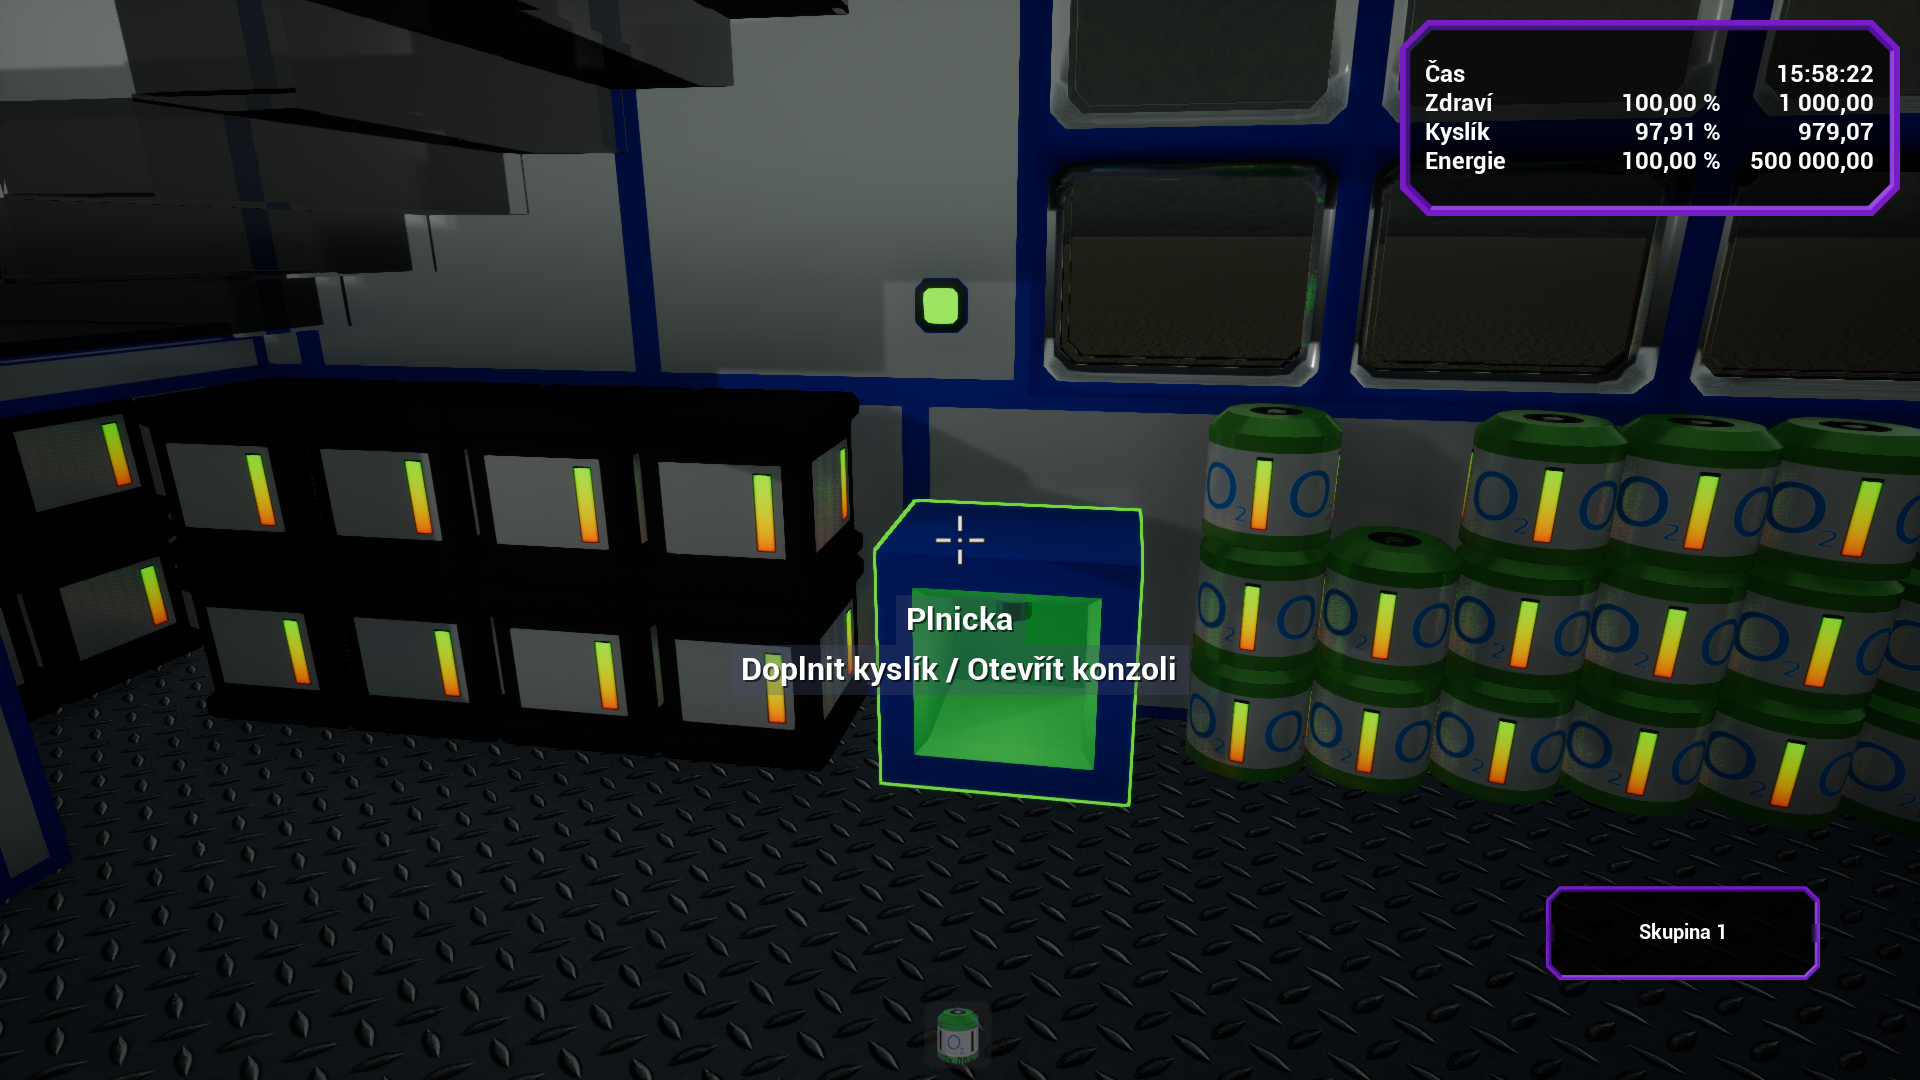
\includegraphics[ width=140mm]{../img/user/filler/0use}

\caption{Plnička kyslíkové bomby -- náhled}
\label{fig:user_filler_0use}

\end{figure}

\FloatBarrier

Ta má v~levé části přiřazený ovladač, případně je možné nejvýše jeden ovladač ze seznamu ovladačů přiřadit. Pokud je přiřazen ovladač, zapnutí bloku se řídí jeho nastavením. V~pravé části je možné regulovat spotřebovávanou energii.

Uprostřed je možné vybrat bomby, které jsou v~inventáři hráče, k~naplnění.

\begin{figure}[!ht]\centering
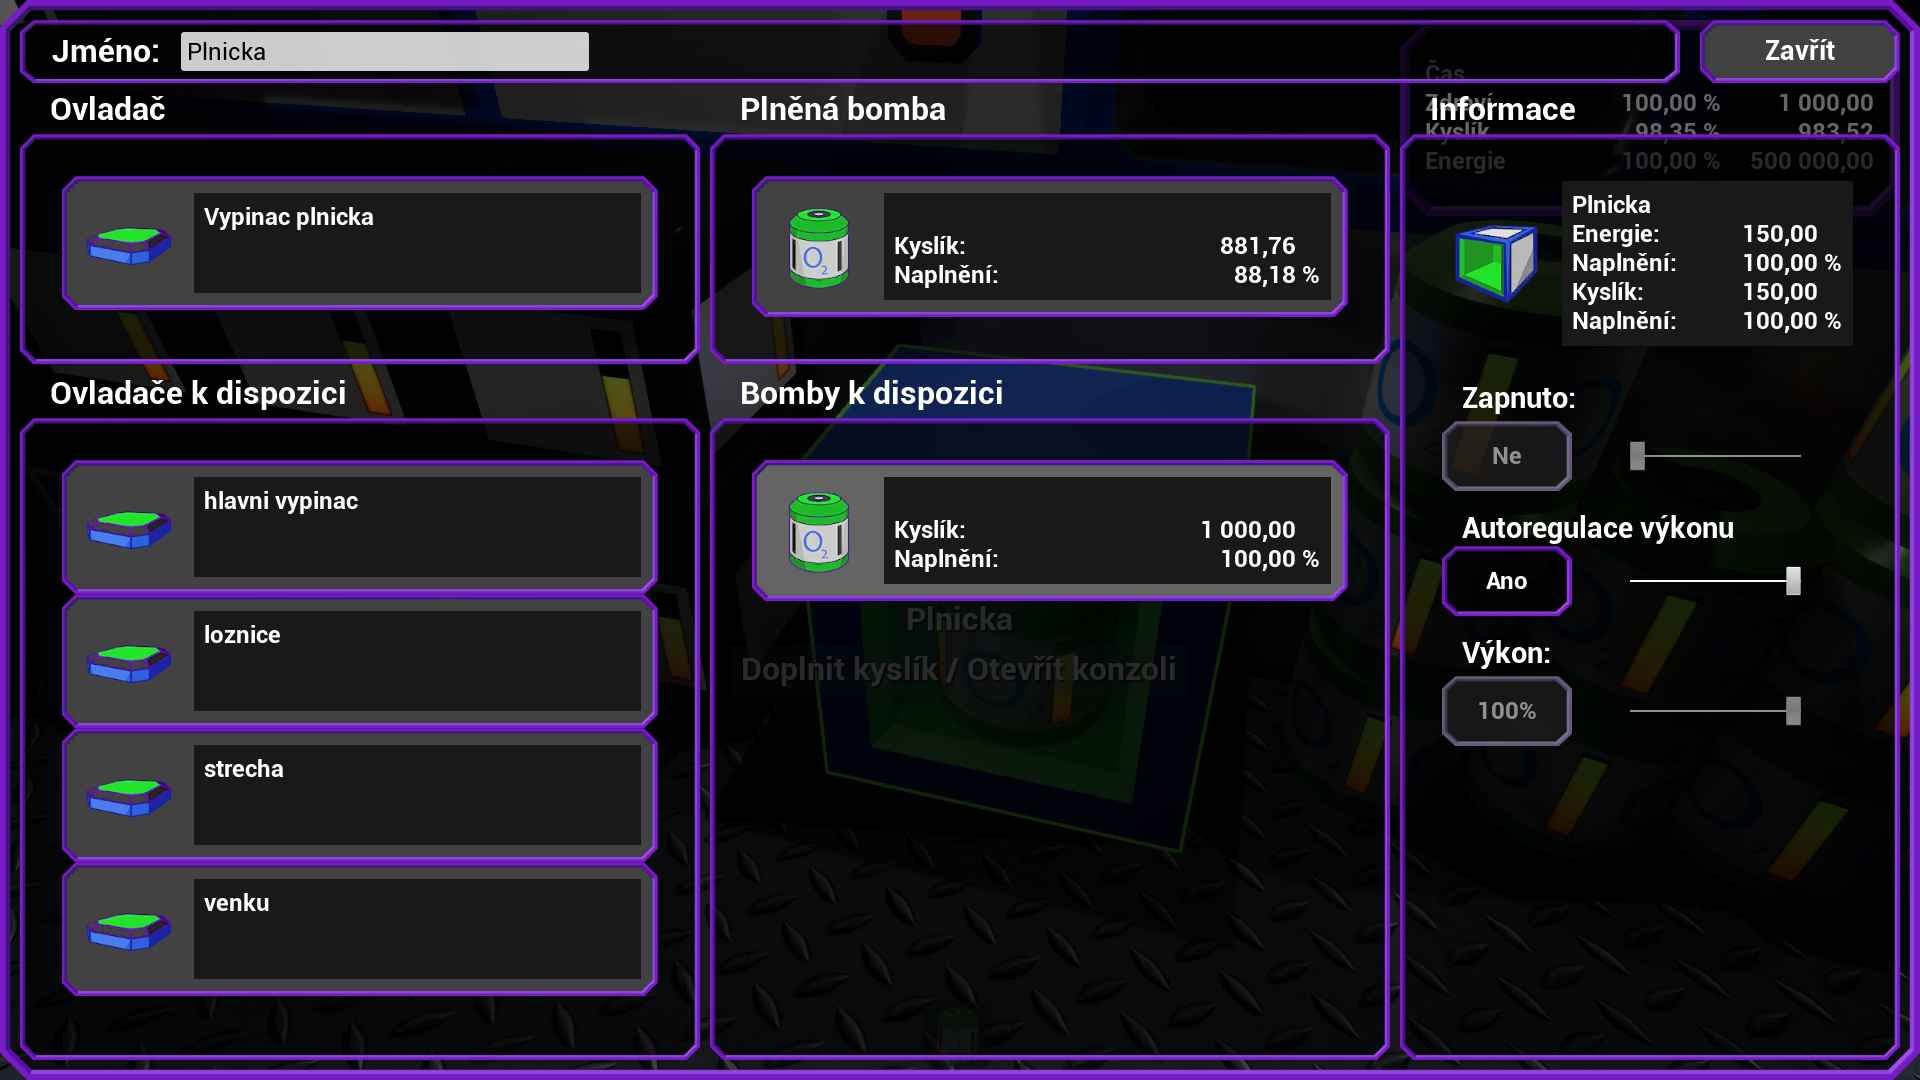
\includegraphics[ width=140mm]{../img/user/filler/1fill}

\caption{Plnička kyslíkové bomby -- ovládací obrazovka}
\label{fig:user_filler_1fill}

\end{figure}

\FloatBarrier

Pokud je plnička zapnuta, generuje kyslík a~ze své zásoby plní přiřazenou kyslíkovou bombu.

\begin{figure}[!ht]\centering
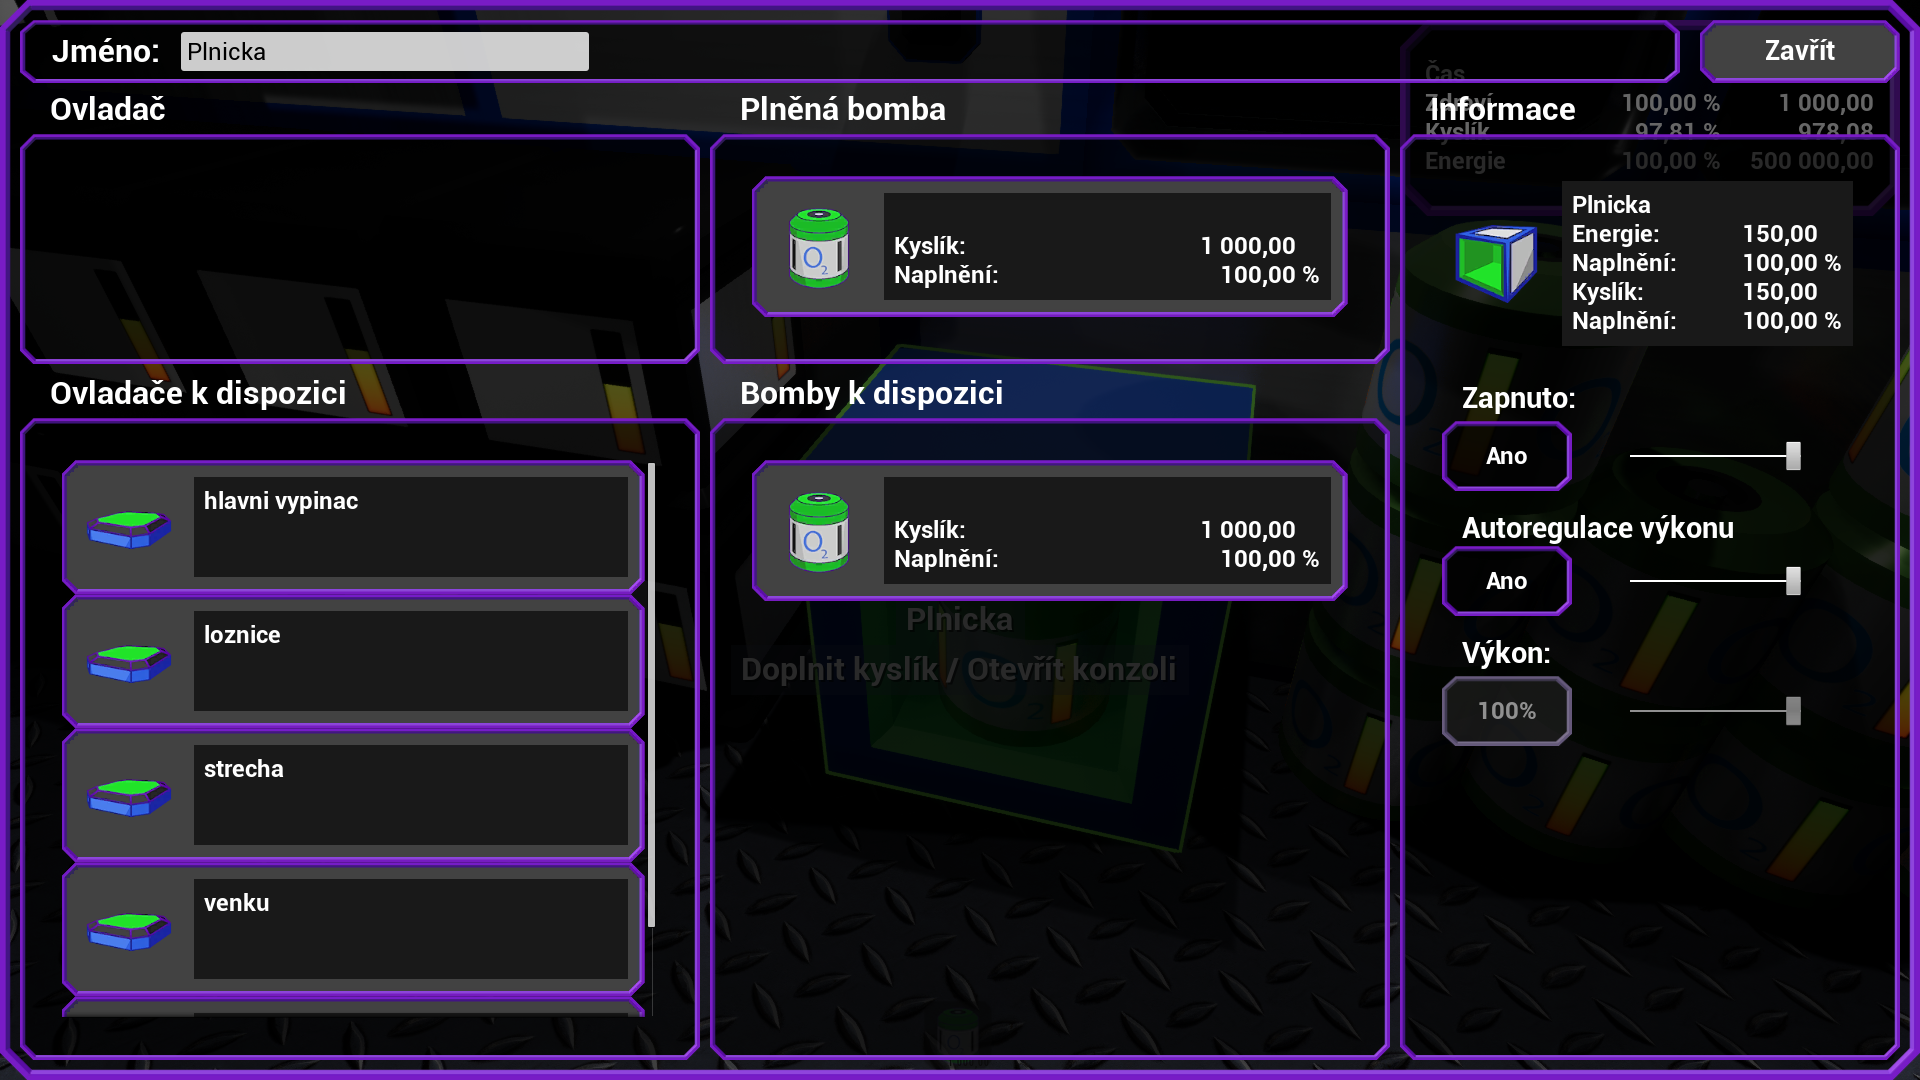
\includegraphics[ width=140mm]{../img/user/filler/2filled}

\caption{Plnička kyslíkové bomby -- naplněno}
\label{fig:user_filler_2filled}

\end{figure}



\FloatBarrier
%!TEX root = ../prace.tex

\section{Přepínač}

Přepínač slouží jako ovládání pro světla a plničku

\begin{figure}[!h]\centering
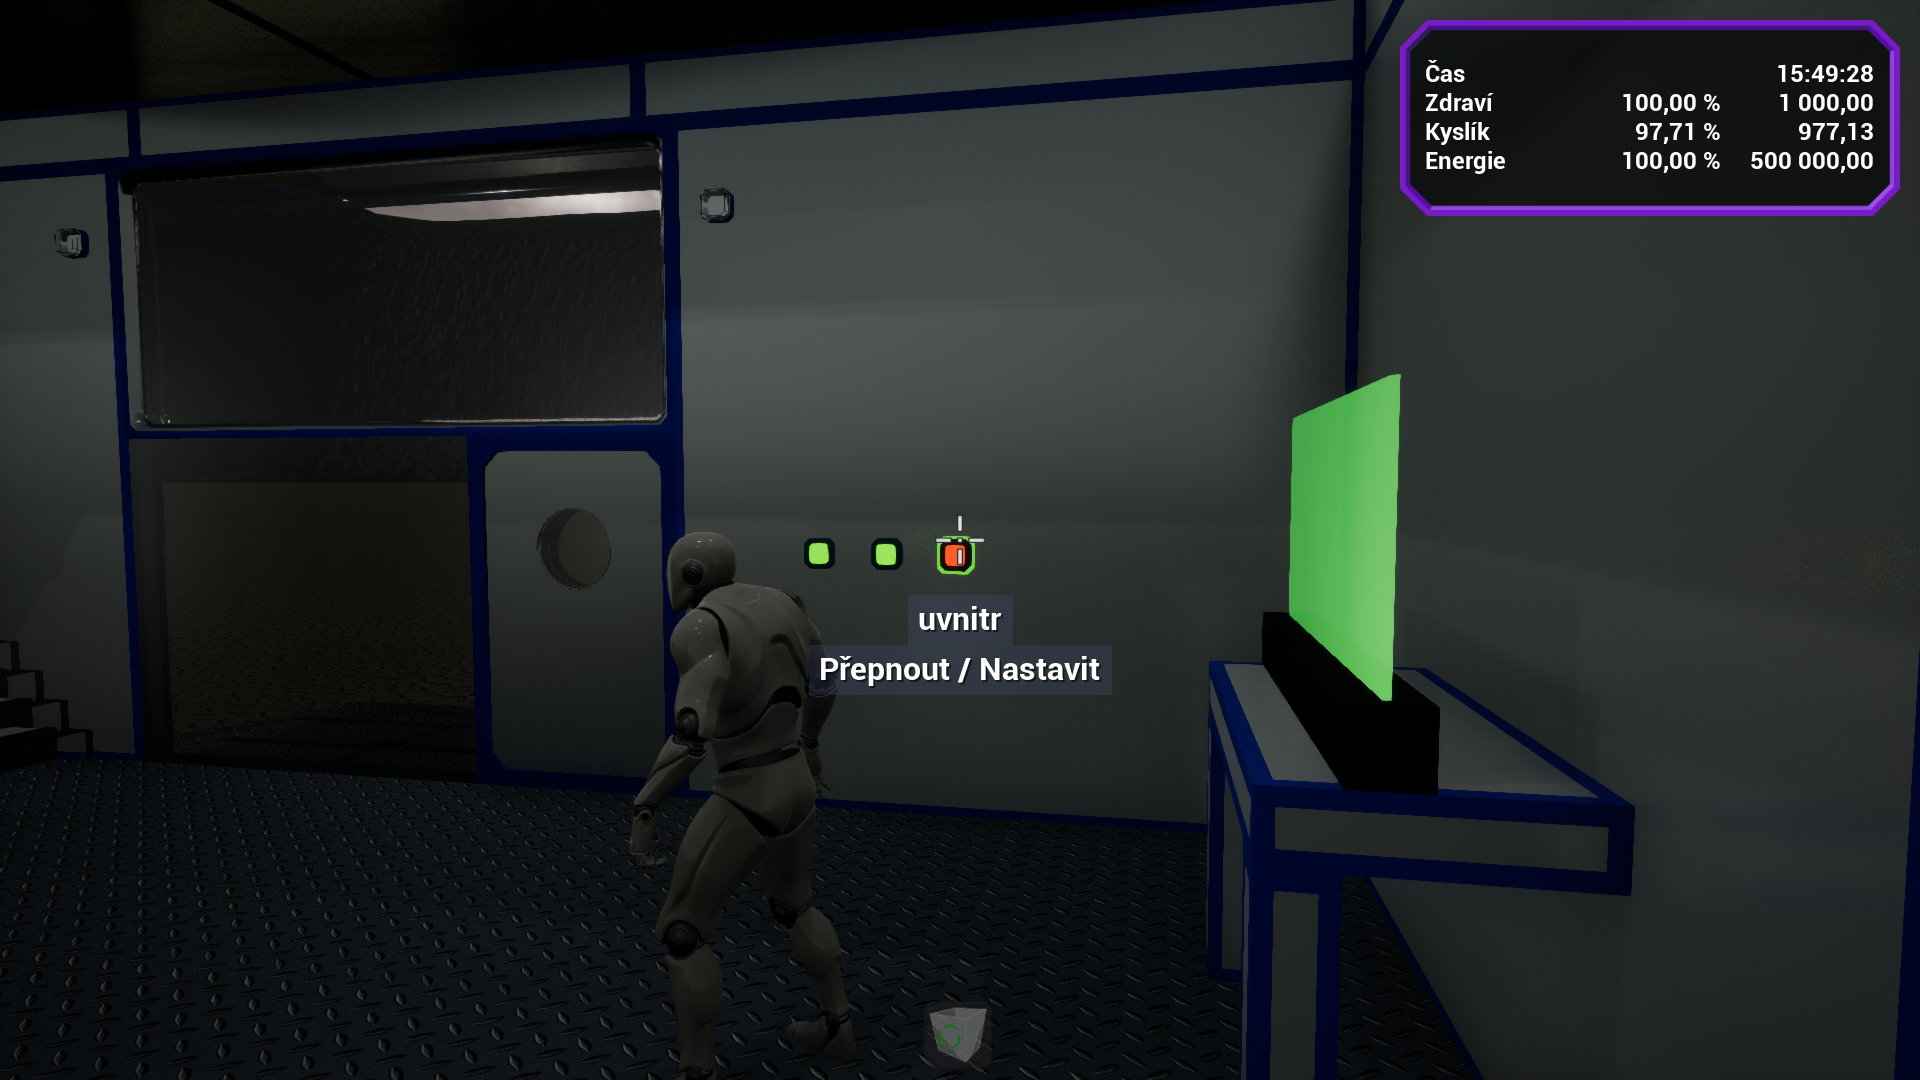
\includegraphics[ width=140mm]{../img/user/switcher/0switcherGeneral}

\caption{Přepínač - den}
\label{fig:user_switcher_0switcherGeneral}

\end{figure}

\FloatBarrier

Blok umožňuje reagovat na denní dobu - automatické přepínání na definovaný stav, pokud začne den, nebo začne noc.

V levé části le možné přiřazovat ovládané bloky

\begin{figure}[!h]\centering
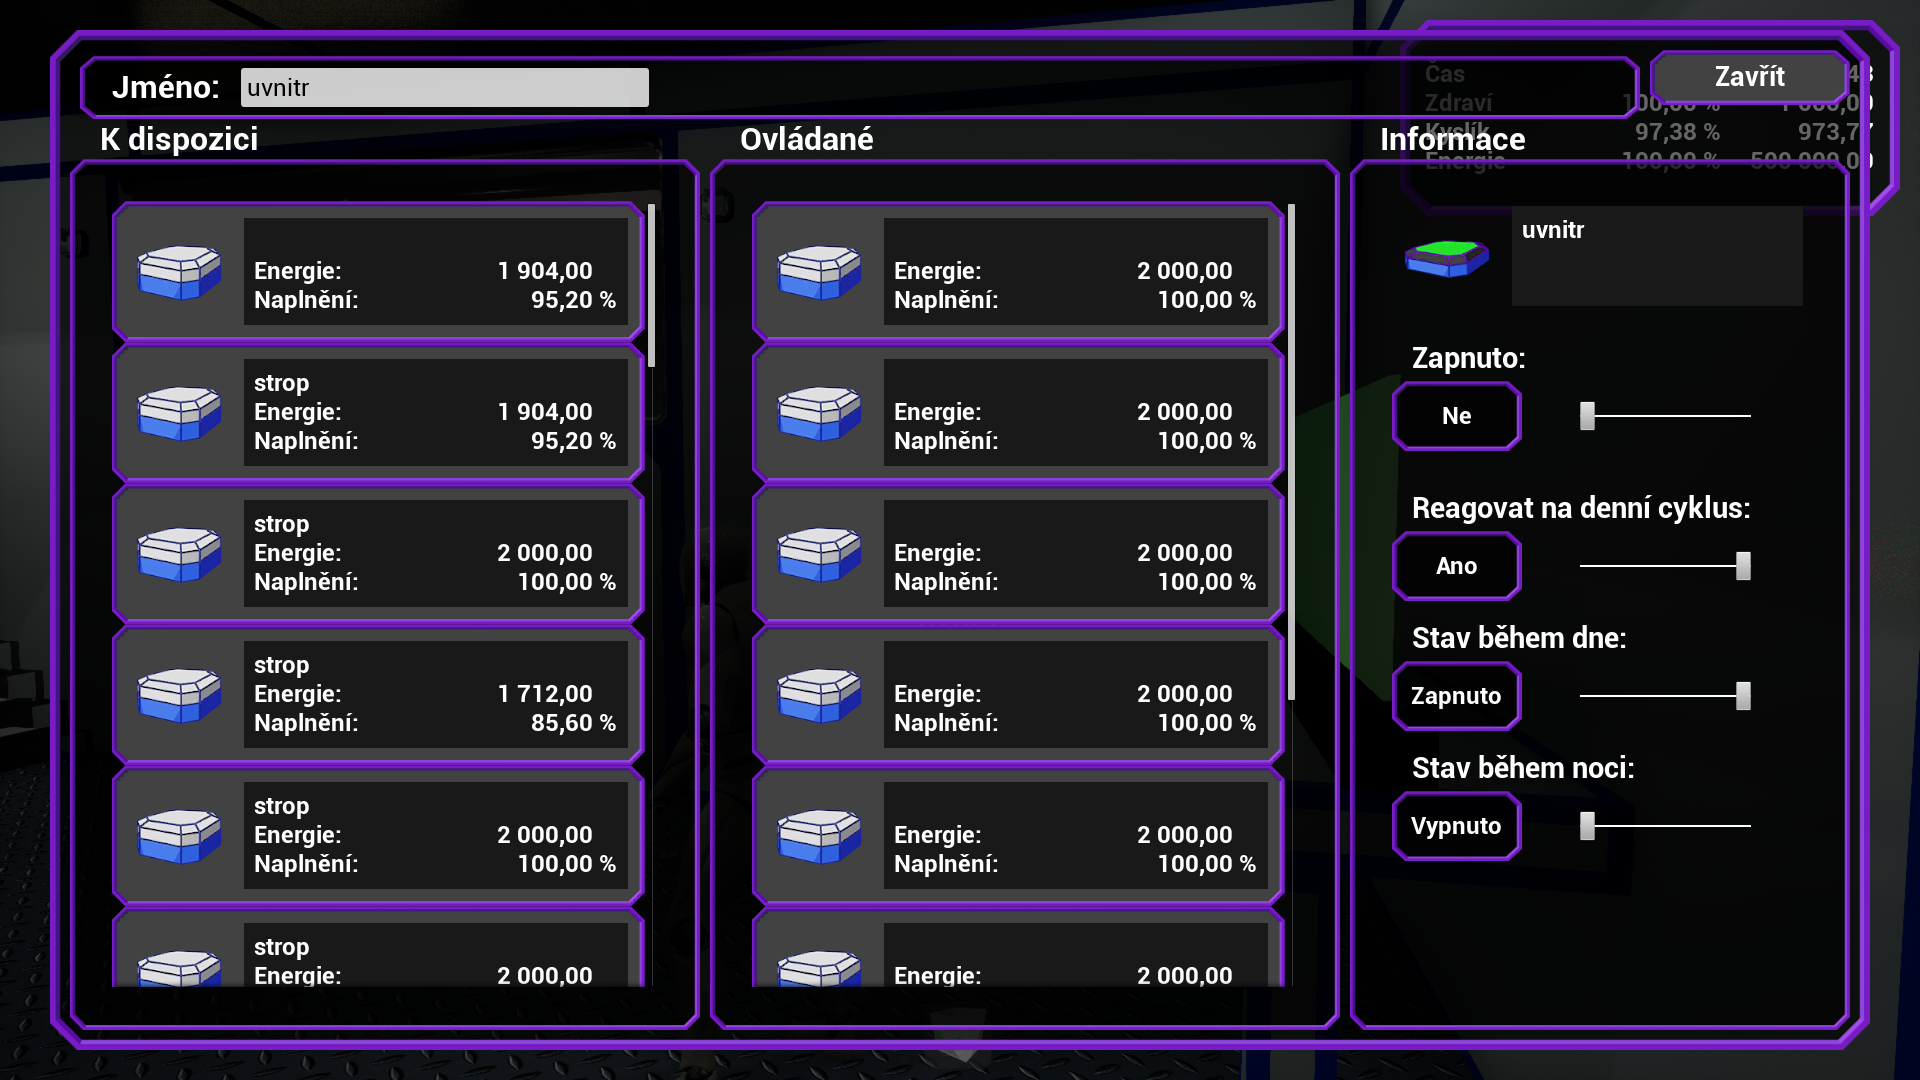
\includegraphics[ width=140mm]{../img/user/switcher/switcherControls}

\caption{Přepínač - poledne, zataženo}
\label{fig:user_switcher_switcherControls}

\end{figure}


\FloatBarrier
%!TEX root = ../prace.tex

\section{Světlo}

Světlo má podobné rozhraní jako Plnička. V levé části se přiřazuje ovladač, v pravé se edituje výkon bloku.

\begin{figure}[!ht]\centering
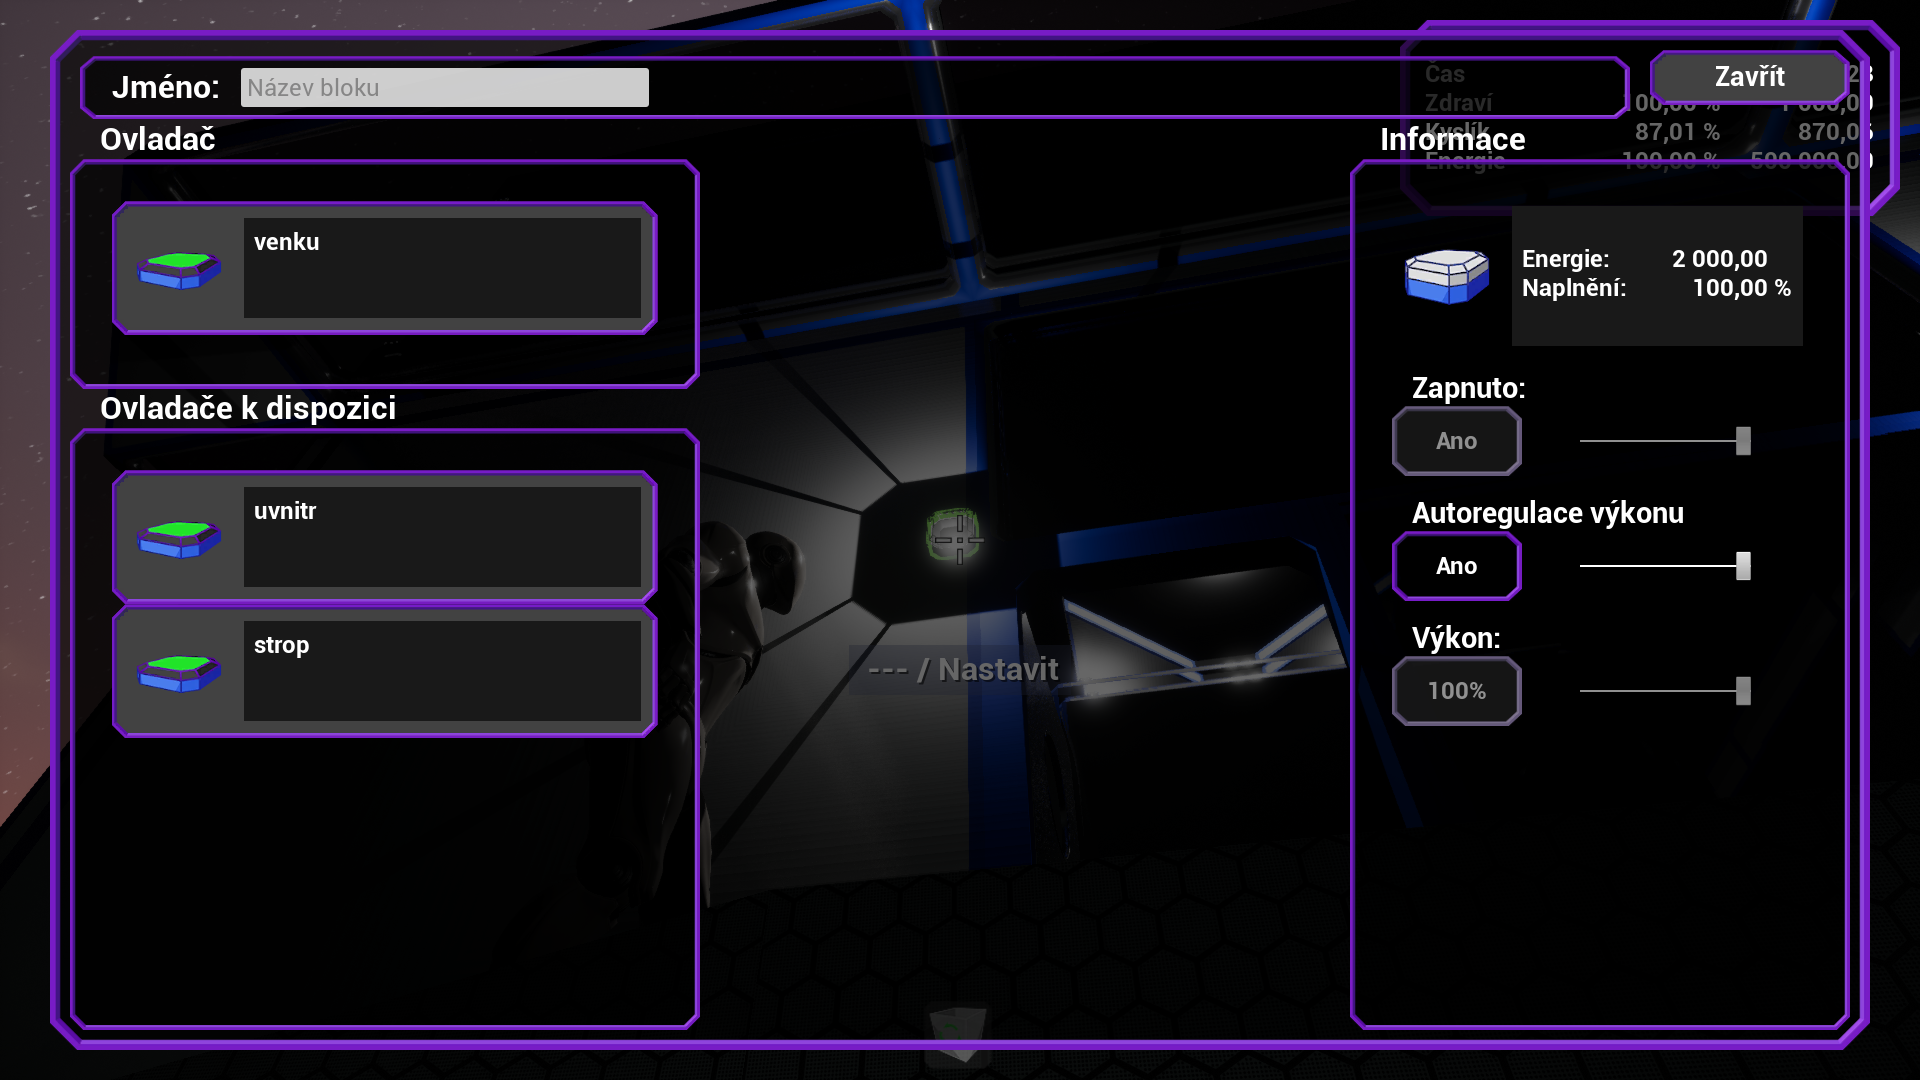
\includegraphics[ width=140mm]{../img/user/light/0light}

\caption{Světlo - ovládací obrazovka}
\label{fig:user_light_0light}

\end{figure}

\FloatBarrier

%!TEX root = ../prace.tex

\section{Kyselý déšť}

Pokud se blíží bouře kyselého deště, nebo právě jedna probíhá, hráč vidí v levé horní části obrazovky zprávu s odhadovaným časem a intenzitou.

To umožňuje strategicky řídit chod svých budov a případně limitovat spotřebovávané zdroje v případě očekávaných dlouhotrvajících bouří. Odhadovaný čas je udán v herním čase.

\begin{figure}[!ht]\centering
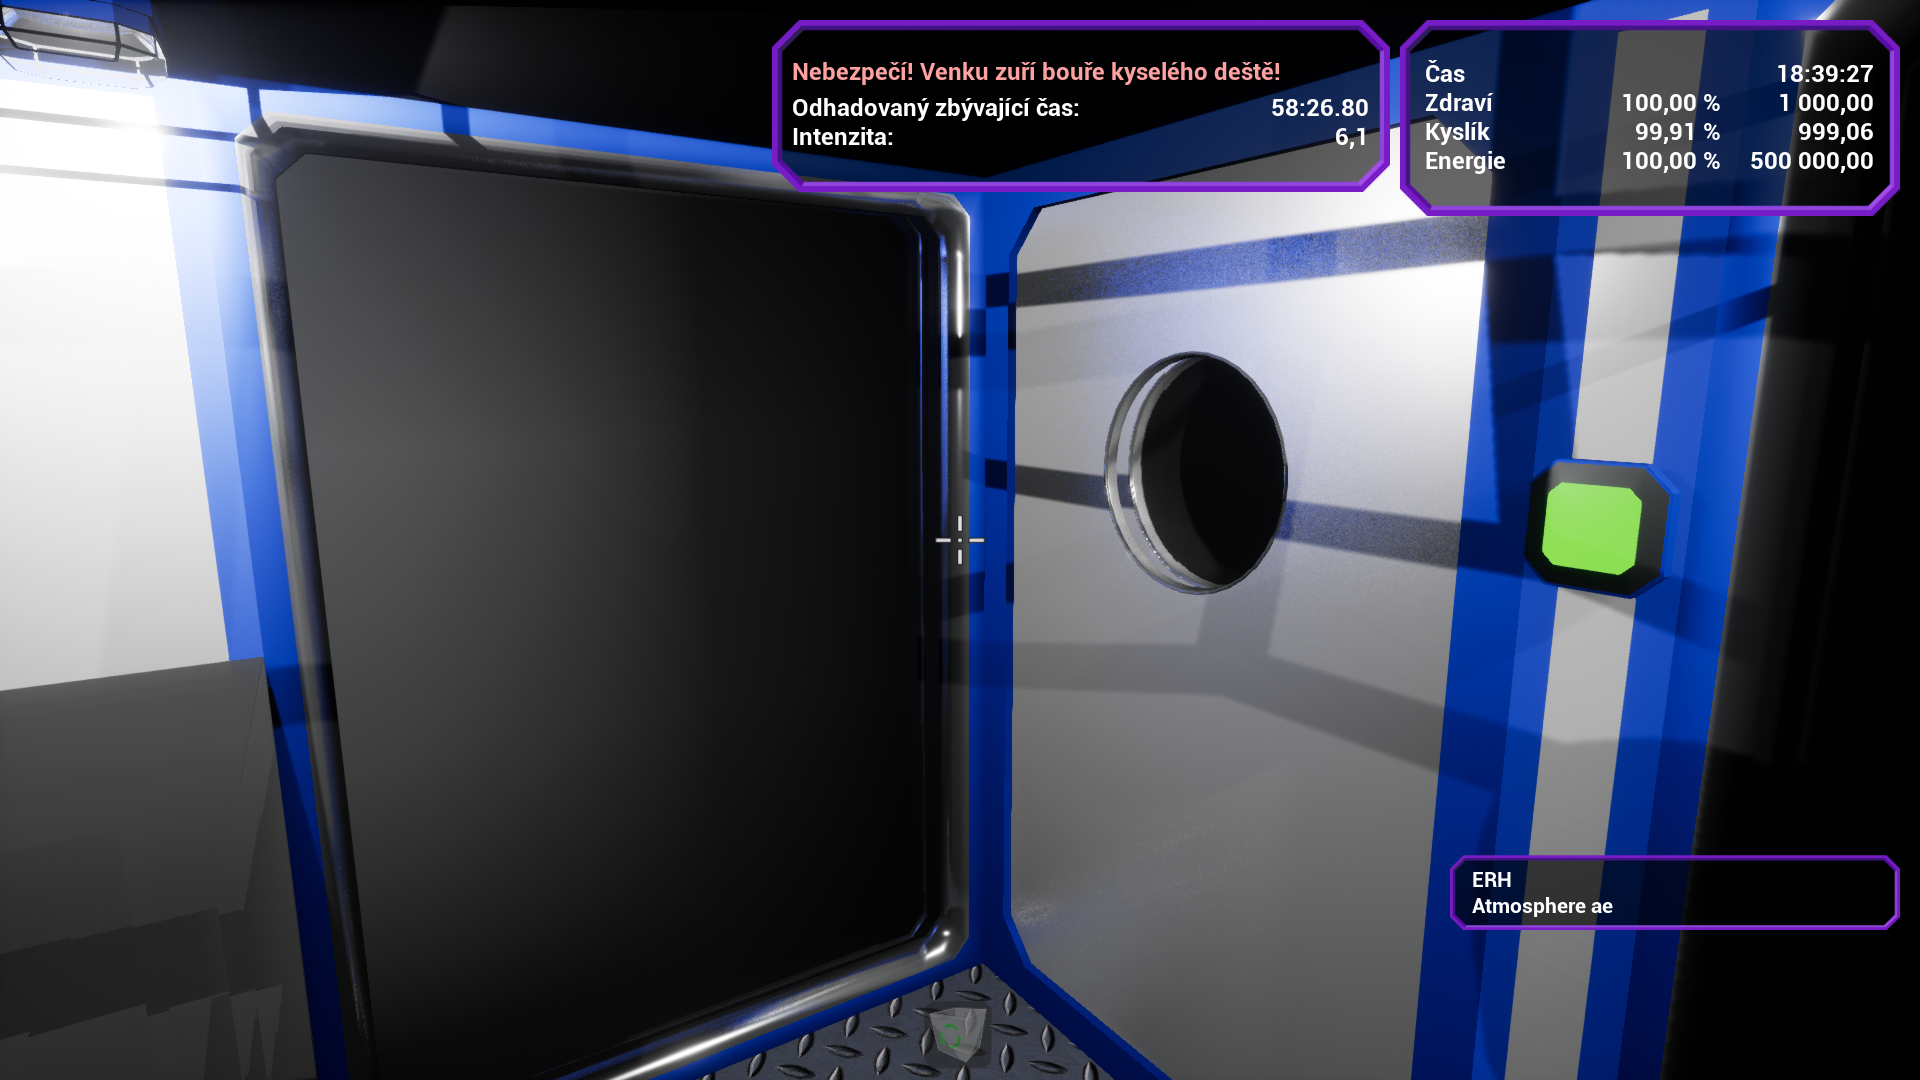
\includegraphics[ width=140mm]{../img/user/rain/0rainInfo}

\caption{Kyselý déšť - info}
\label{fig:user_rain_0rainInfo}

\end{figure}

\FloatBarrier

Pokud hráč není ukrytý v budově či pod nějakým blokem, dostává zásahy. Dokud má dostatek energie, je schopen odolávat účinkům bouře, v momentě, kdy mu energie dojde, začne mu ubývat zdraví.


\begin{figure}[!ht]\centering
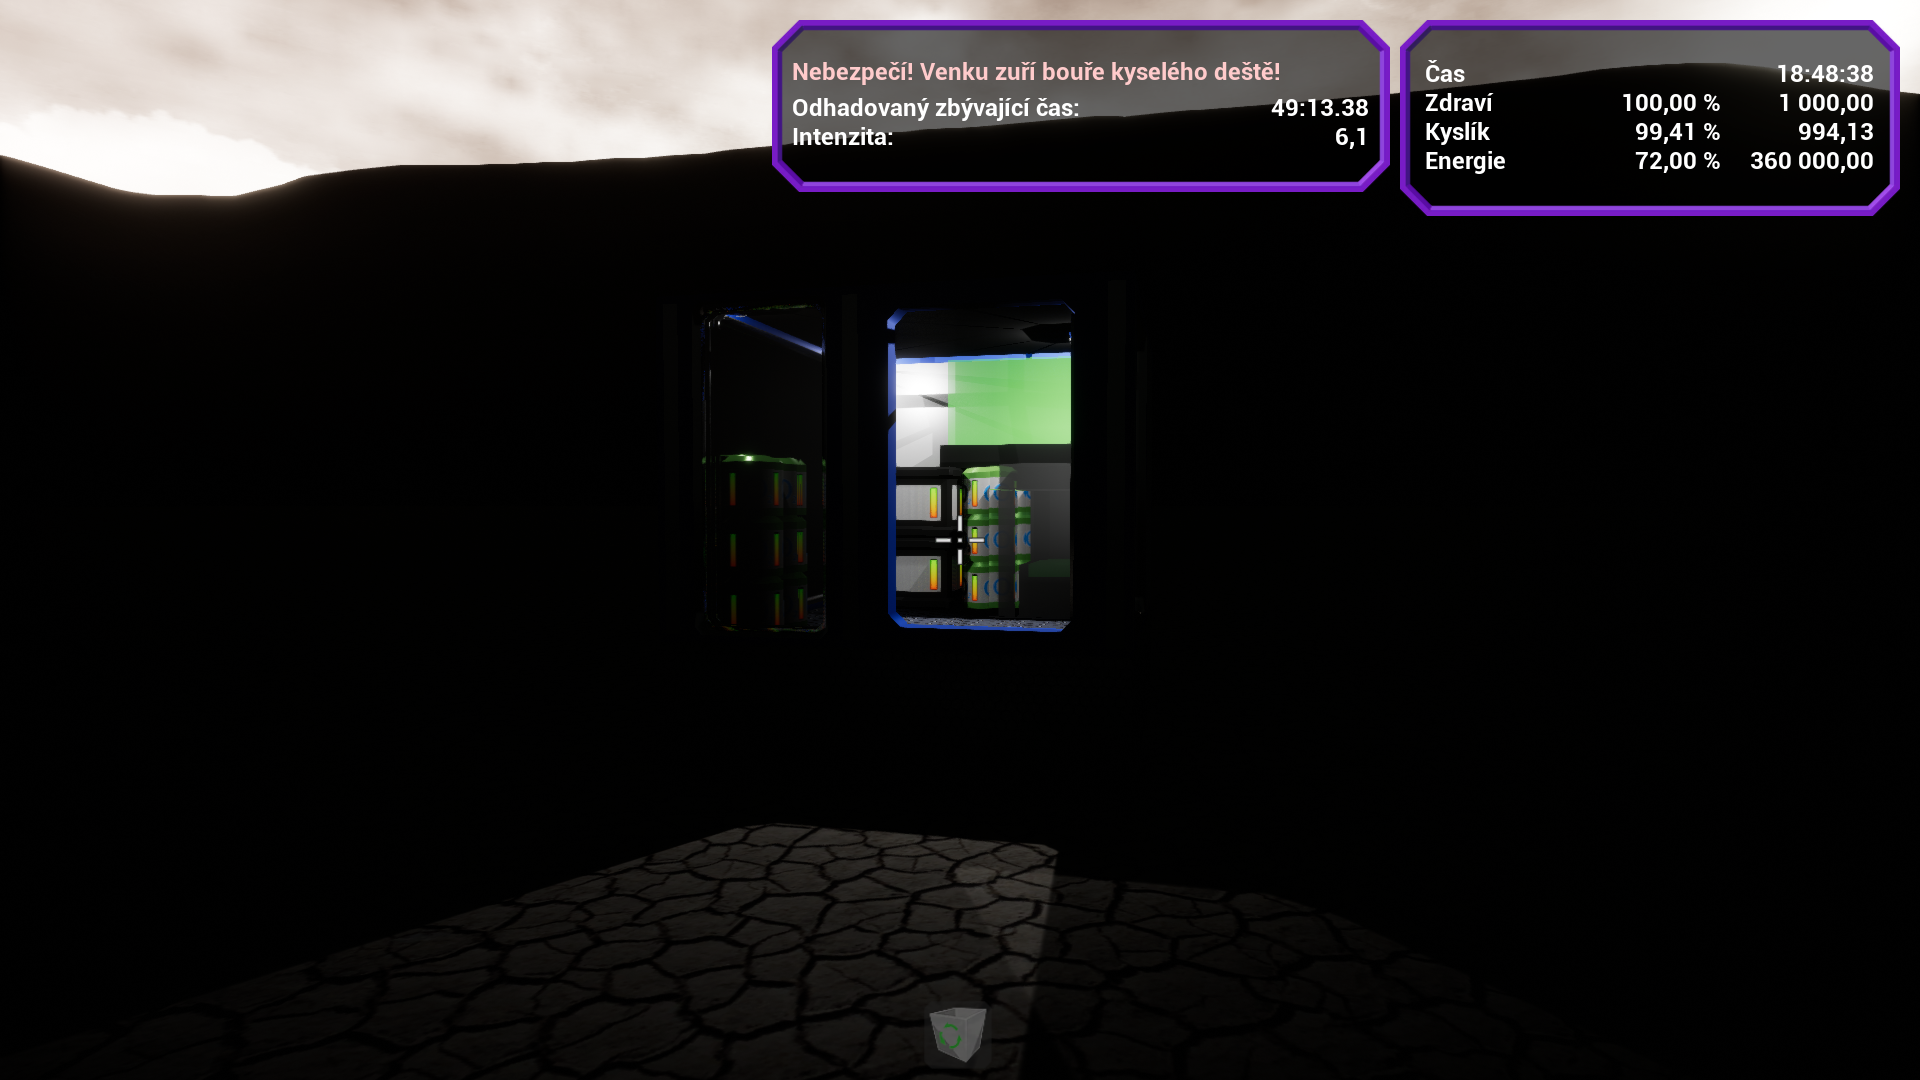
\includegraphics[ width=140mm]{../img/user/rain/1rainDamage}

\caption{Kyselý déšť - zásahy}
\label{fig:user_rain_1rainDamage}

\end{figure}

\FloatBarrier

Pokud si hráč doplní energii, začne se mu zdraví obnovovat.

\begin{figure}[!ht]\centering
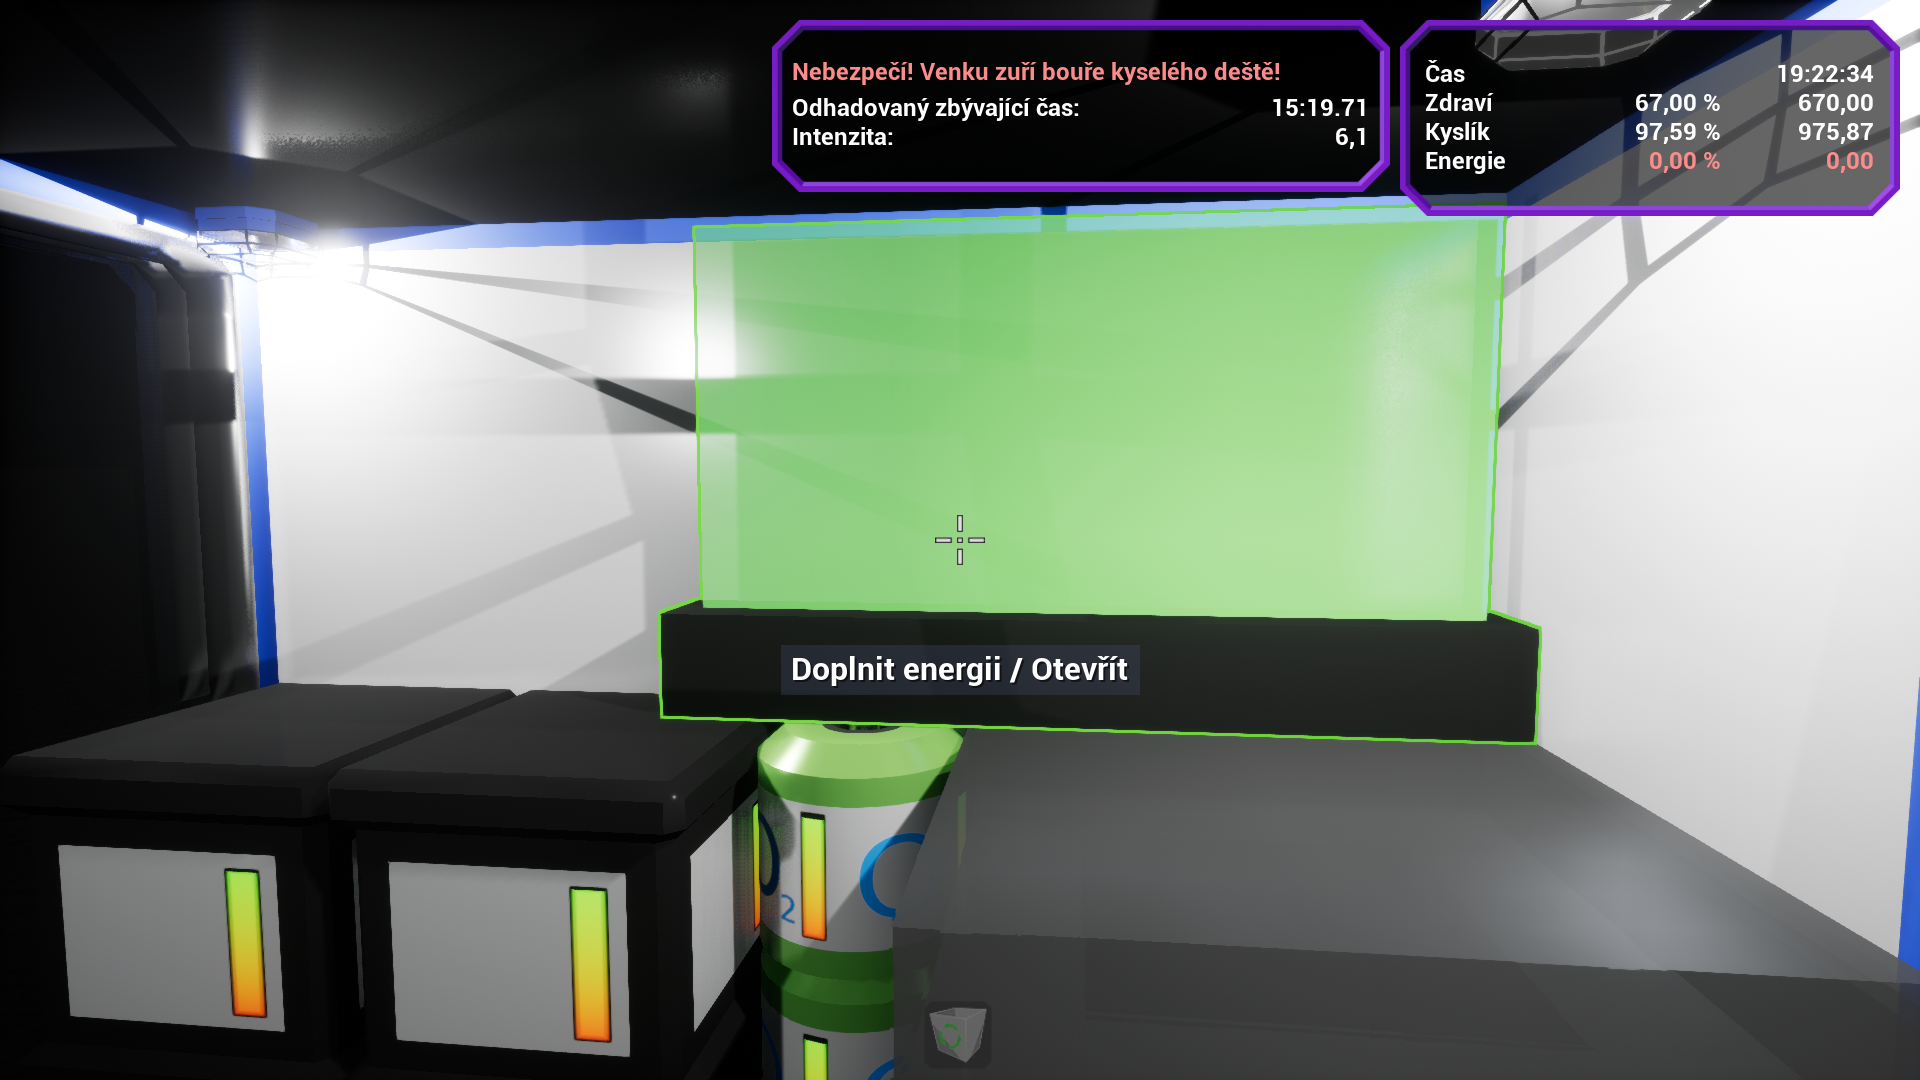
\includegraphics[ width=140mm]{../img/user/rain/2rainRefill}

\caption{Kyselý déšť - obnova zdraví}
\label{fig:user_rain_2rainRefill}

\end{figure}


\begin{figure}[!ht]\centering
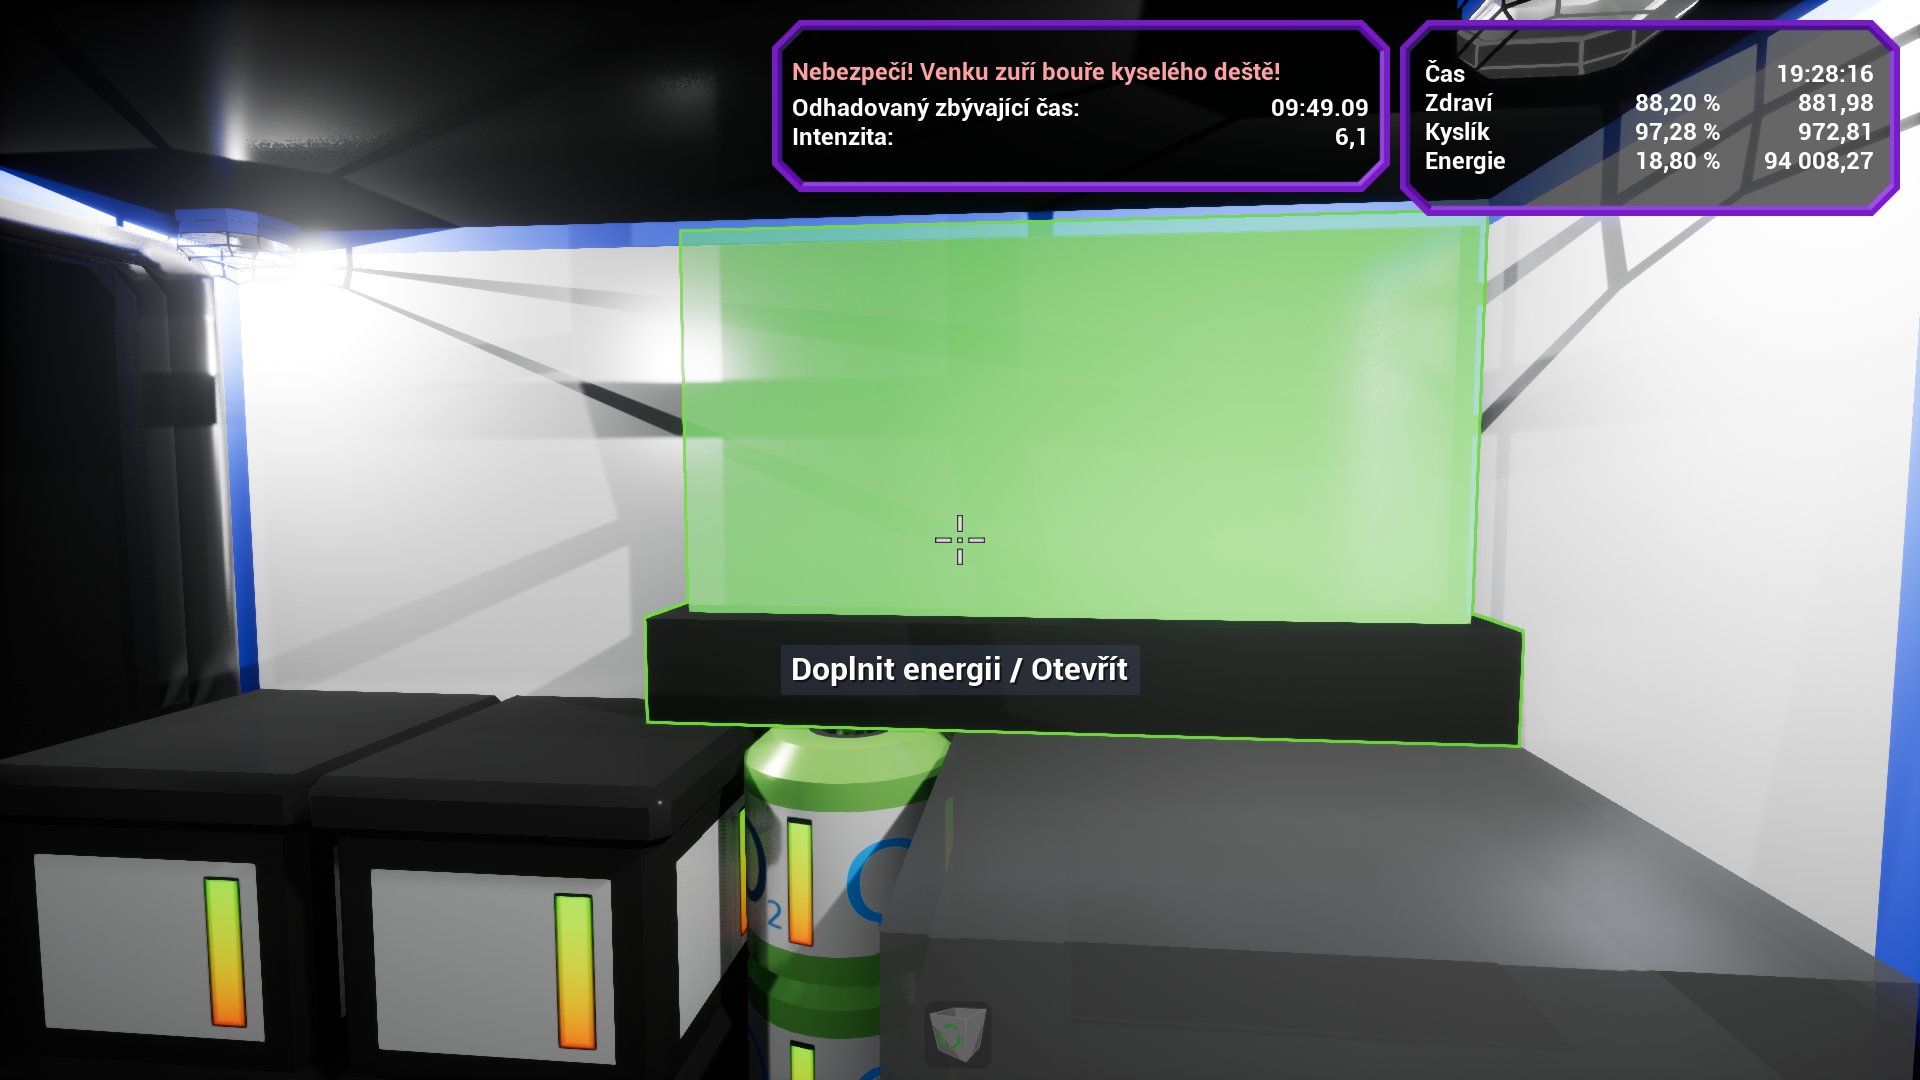
\includegraphics[ width=140mm]{../img/user/rain/3rainRefill1}

\caption{Kyselý déšť - obnova zdraví}
\label{fig:user_rain_3rainRefill1}

\end{figure}

\FloatBarrier

Během bouře je též možné pozorovat animaci generátoru energie, kdy je po každém zásahu rozsvícen příslušný čtverec. Tuto animaci lze z menu vypnout a pokud má uživatel slabší stroj, tak to i doporučujeme.

\begin{figure}[!ht]\centering
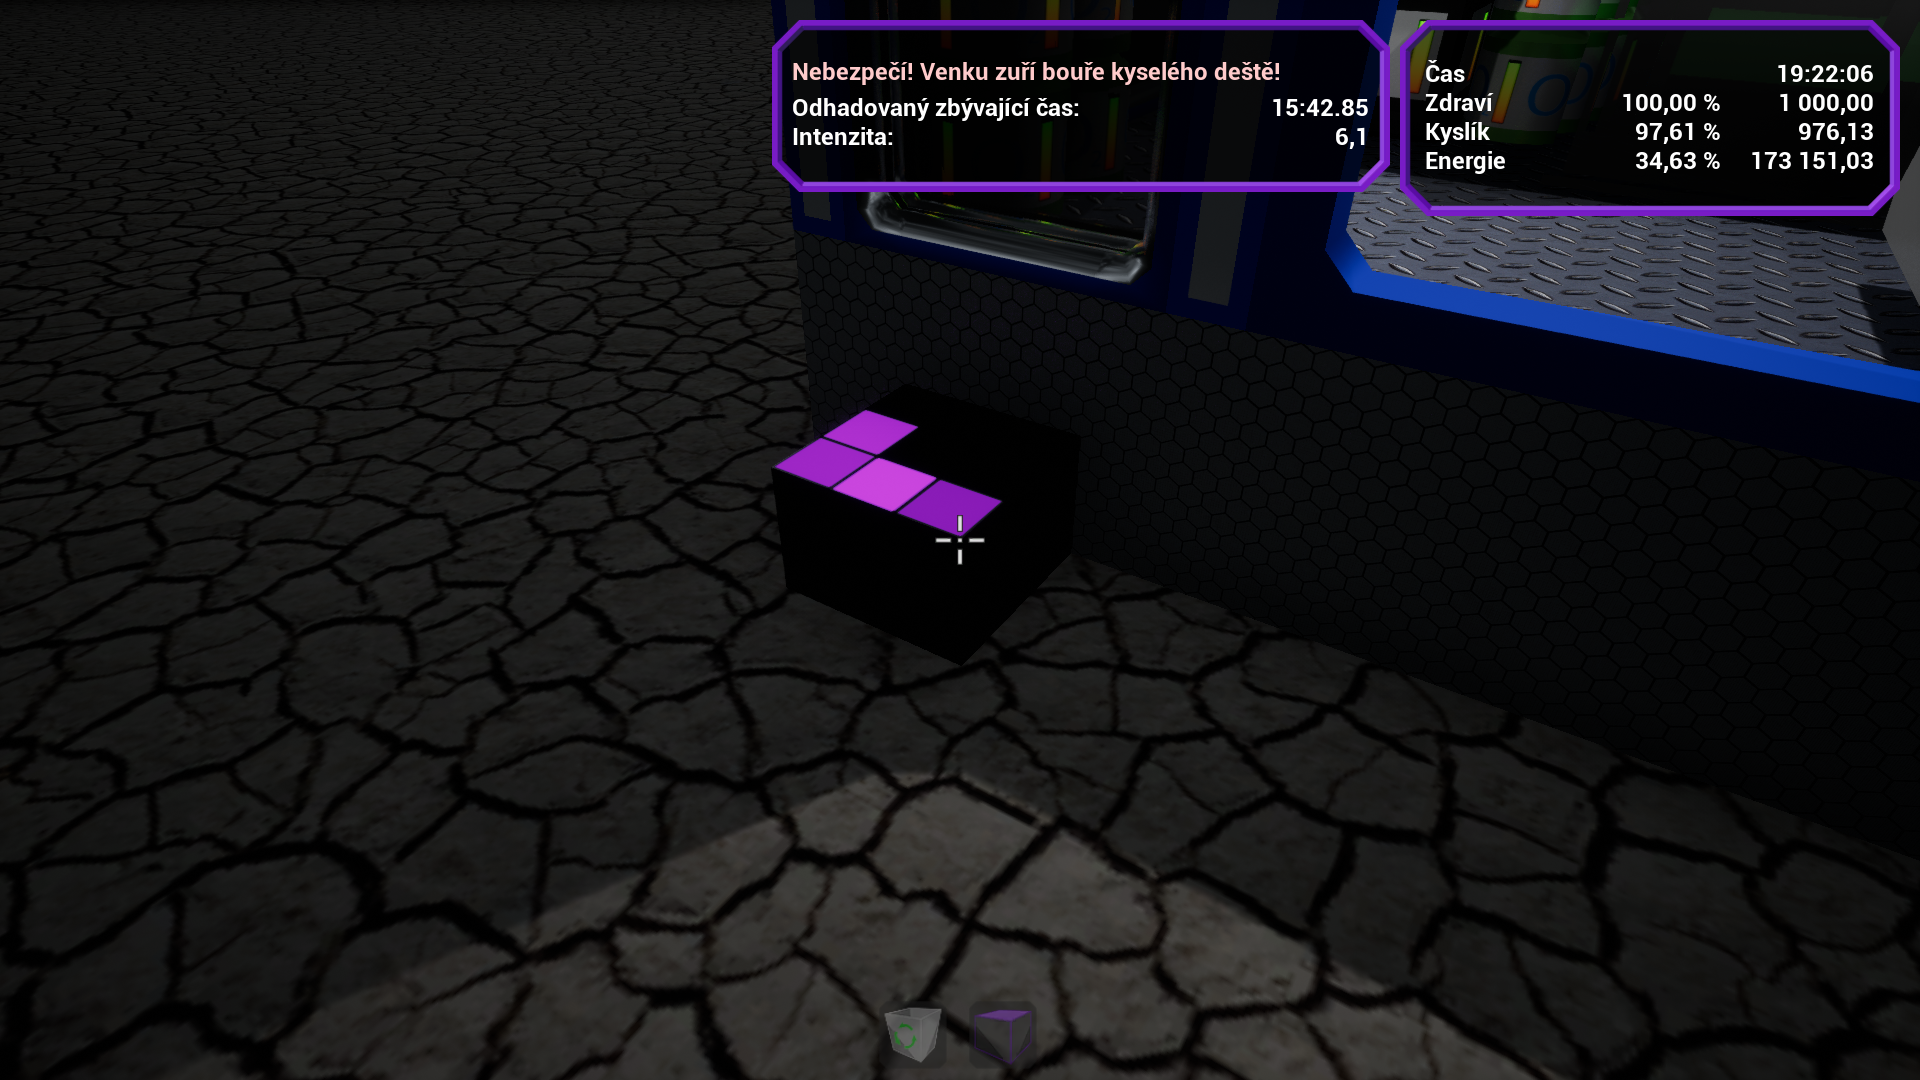
\includegraphics[ width=140mm]{../img/user/rain/4rainGeneratorAnim}

\caption{Kyselý déšť - animace zásahů}
\label{fig:user_rain_4rainGeneratorAnim}

\end{figure}


\FloatBarrier




%!TEX root = ../prace.tex

\chapter{Závěr}


\section{Zhodnocení práce}


\section{Budoucí práce}


\begin{itemize}
	\item dynamičtějí mřížka? 20cm je nejspíše dost málo a vyžaduje to dost preciznosti // TODO zkusit pro test 25 či 30 cm a patřičným způsobem upravit velikosti modelů? (nejspíše to musí zůstat hardcoded, ale zkusím se nad tím zamyslet, pokud bude čas)
	\item vlastní sortování v seznamech

\end{itemize}

TODO dotazník?

%%% Seznam použité literatury
%%% Seznam použité literatury (bibliografie)
%%%
%%% Pro vytváření bibliografie používáme bibTeX. Ten zpracovává
%%% citace v textu (např. makro \cite{...}) a vyhledává k nim literaturu
%%% v souboru literatura.bib.
%%%
%%% Příkaz \bibliographystyle určuje, jakým stylem budou citovány odkazy
%%% v textu. V závorce je název zvoleného souboru .bst. Styly plainnat
%%% a unsrt jsou standardní součástí latexových distribucí. Styl czplainnat
%%% je dodáván s touto šablonou a bibTeX ho hledá v aktuálním adresáři.

\bibliographystyle{czplainnat}    %% Autor (rok) s českými spojkami
% \bibliographystyle{plainnat}    %% Autor (rok) s anglickými spojkami
% \bibliographystyle{unsrt}       %% [číslo]

\renewcommand{\bibname}{Seznam použité literatury}

%%% Vytvoření seznamu literatury. Pozor, pokud jste necitovali ani jednu
%%% položku, seznam se automaticky vynechá.

\bibliography{literatura}

%%% Kdybyste chtěli bibliografii vytvářet ručně (bez bibTeXu), lze to udělat
%%% následovně. V takovém případě se řiďte normou ISO 690 a zvyklostmi v oboru.

% \begin{thebibliography}{99}
%
% \bibitem{lamport94}
%   {\sc Lamport,} Leslie.
%   \emph{\LaTeX: A Document Preparation System}.
%   2. vydání.
%   Massachusetts: Addison Wesley, 1994.
%   ISBN 0-201-52983-1.
%
% \end{thebibliography}


%%% Obrázky v bakalářské práci
%%% (pokud jich je malé množství, obvykle není třeba seznam uvádět)
\listoffigures

%%% Tabulky v bakalářské práci (opět nemusí být nutné uvádět)
%%% U matematických prací může být lepší přemístit seznam tabulek na začátek práce.
%\listoftables

%%% Použité zkratky v bakalářské práci (opět nemusí být nutné uvádět)
%%% U matematických prací může být lepší přemístit seznam zkratek na začátek práce.

% Soubor se všemi zkratkami uvedenými v práci

%!TEX root = prace.tex


\chapter*{Seznam použitých zkratek}
\addcontentsline{toc}{chapter}{Seznam použitých zkratek}

TODO seznam zkratek

%%% Přílohy k bakalářské práci, existují-li. Každá příloha musí být alespoň jednou
%%% odkazována z vlastního textu práce. Přílohy se číslují.
%%%
%%% Do tištěné verze se spíše hodí přílohy, které lze číst a prohlížet (dodatečné
%%% tabulky a grafy, různé textové doplňky, ukázky výstupů z počítačových programů,
%%% apod.). Do elektronické verze se hodí přílohy, které budou spíše používány
%%% v elektronické podobě než čteny (zdrojové kódy programů, datové soubory,
%%% interaktivní grafy apod.). Elektronické přílohy se nahrávají do SISu a lze
%%% je také do práce vložit na CD/DVD. Povolené formáty souborů specifikuje
%%% opatření rektora č. 23/2016.
\chapwithtoc{Přílohy}

\openright
\end{document}
